\documentclass[12pt]{book}
\usepackage{geometry}                % See geometry.pdf to learn the layout options. There are lots.
\geometry{a4paper}                   % ... or a4paper or a5paper or ... 
%\geometry{landscape}                % Activate for for rotated page geometry
%\usepackage[parfill]{parskip}    % Activate to begin paragraphs with an empty line rather than an indent
\usepackage{graphicx}
\usepackage{amssymb}
\usepackage{amsmath}
\usepackage{epstopdf}
\usepackage{caption}
\usepackage{subcaption}
\usepackage[english]{babel}
\usepackage[T1]{fontenc}
\usepackage{epstopdf}
\usepackage[utf8]{inputenc}
\usepackage{units}
\usepackage[toc,page]{appendix}
\usepackage[section]{placeins}
\usepackage[percent]{overpic}
%\usepackage{titling}
\usepackage{cite}
\usepackage{nicefrac}
\usepackage{xcolor}
\usepackage{tikz}
\usepackage{standalone}
\usepackage{siunitx}
\usepackage{multirow}
\usepackage{booktabs}
\usetikzlibrary{shapes,arrows,calc,fadings}
\usetikzlibrary{trees}
\usetikzlibrary{shadows.blur}
\usetikzlibrary{positioning}
\usetikzlibrary{decorations.pathmorphing}
\usetikzlibrary{decorations.markings}
\usepackage{breakcites}


\newcommand \dd[1]  { \,\textrm d{#1}   }
\pagestyle{plain}

\usepackage{hyperref}
\usepackage{url}
\newcommand{\subtitle}[1]{%
  \posttitle{%
    \par\end{center}
    \begin{center}\large#1\end{center}
    \vskip0.5em}%
}
\RequirePackage{lineno}
\setlength{\linenumbersep}{6pt}
%\linenumbers

%\title{Jet quenching in fluctuating events in heavy-ion collisions}
%\title{Particle Identified Flow and Unfolding in Heavy Ion Collisions}
%\subtitle{Master's thesis}
%\author{Tomas Snellman}
%\date{}                                           % Activate to display a given date or no date

\include{defs}
\begin{document}

%!TEX root = Thesis.tex


%%%%%%%%%%%%%%%%%%%%%%%%%%%%%%%%%%%%%%%%%%%%%%%%
%                            Front (Title) page
%%%%%%%%%%%%%%%%%%%%%%%%%%%%%%%%%%%%%%%%%%%%%%%%

\thispagestyle{empty}
\vspace*{10mm}

\centerline{DEPARTMENT OF PHYSICS, UNIVERSITY OF JYV\"ASKYL\"A}
\centerline{RESEARCH REPORT No. ??/2019}

\vspace{25mm} 

\centerline{\bf JET TRANSVERSE MOMENTUM DISTRIBUTIONS }
\centerline{\bf  FROM RECONSTRUCTED JETS}

\centerline{\bf  IN P--PB COLLISIONS AT \sqrtSnnE{5.02}}
\centerline{\bf }
%JET TRANSVERSE MOMENTUM DISTRIBUTIONS FROM RECONSTRUCTED JETS IN P--PB COLLISIONS AT \sqrtSnnE{5.02}
\vspace{13mm}


\centerline{\bf BY}
\centerline{\bf TOMAS SNELLMAN}

\vspace{13mm}

\centerline{Academic Dissertation}
\centerline{for the Degree of}
\centerline{Doctor of Philosophy}

\vspace{13mm}

%\centerline{To be presented, by permission of the}
%\centerline{Faculty of Mathematics and Natural Sciences}
%\centerline{of the University of Jyv\"askyl\"a,}
%\centerline{for public examination in Auditorium FYS 1 of the}
%\centerline{University of Jyv\"askyl\"a on June 19th, 2019,}
%\centerline{at 12 o'clock noon}

\centerline{\emph{
To be presented, by permission of the Faculty of Mathematics and Natural Sciences}}
\centerline{\emph{
 of the University of Jyv\"askyl\"a, for public examination in Auditorium FYS 1}}
 \centerline{\emph{ of the University of Jyv\"askyl\"a on June 19th, 2019, at 12 o'clock noon}}

\vspace{13mm}



\centerline{\includegraphics[height=20mm]{Soihtu}}

\centerline{Jyv\"askyl\"a, Finland}
%\centerline{\today}
\centerline{June 2019}
\pagebreak
\thispagestyle{empty}
\section*{Personal Contribution} 
{\color{red} TODO: Correct format and data}
Snellman, Tomas

Jet transverse momentum distributions from reconstructed jets in p--Pb collisions at \sqrtSnnE{5.02}


Jyväskylä; University of Jyväskylä, 2019, ...

Department of Physics Research Report No. xx/2019

ISSN
ISBN
ISBN

Keywords: jet, jet shape, jet fragmentation, jet reconstruction, p--Pb, ALICE,  transverse momentum, CERN, LHC

The main contributions of the author are listed below

\begin{itemize}
\item Jet fragmentation transverse momentum (\jt{}) analysis for  \sqrtSnnE{5.02} p--Pb data
\begin{itemize}
\item Implementation of the observable (\jt{})
\item Implementation and improvement of the perpendicular cone background method
\item Developing the random background method
\item Performing unfolding of detector effects on the data
\item Systematic uncertainty analysis
\item Discussion of the results and comparing data to models and \jt{} extracted from two-particle correlations
\end{itemize}
\item Quality assurance (QA) of the Gas Electron Multiplier (GEM) foils that are built into the Time Projection Chamber (TPC) detector of the ALICE experiment
\end{itemize} 


%%%%%%%%%%%%%%%%%%%%%%%%%%%%%%%%%%%%%%%%%%%%%%%%
%                            Author page
%%%%%%%%%%%%%%%%%%%%%%%%%%%%%%%%%%%%%%%%%%%%%%%%
\pagebreak
\thispagestyle{empty}

\vspace*{25mm} 

\begin{table}[h!]
%\centering
  \begin{tabular}{ p{4cm}  p{6cm} }
  {\bf Author} 	& {Tomas Snellman}\\  
  {} 			& {University of Jyv\"askyl\"a}\\  
  {} 			& {Finland}\\  
  {} 			& {}\\  

  {\bf Supervisors} 	& {Dr.~Kim Dong Jo}\\  
  {} 				& {University of Jyv\"askyl\"a}\\  
  {} 				& {Finland}\\  
  {} 				& {}\\  

  {}			 	& {Prof.~Jan Rak}\\  
  {} 				& {University of Jyv\"askyl\"a}\\  
  {} 				& {Finland}\\  
  {} 				& {}\\  

  {\bf Reviewers} 	& {Prof.~Stefan Bathe}\\  
  {} 				& {Baruch College, CUNY}\\  
  {} 				& {USA}\\  
  {} 				& {}\\  

  {}			 	& {Prof.~Marcin Chrząszcz}\\  
  {} 				& {Instytut Fizyki Jądrowej PAN}\\  
  {} 				& {Poland}\\  
  {} 				& {}\\  
    
  {\bf Opponent} 	& {Prof.~Jamie Nagle}\\  
  {} 				& {University of Colorado Boulder}\\  
  {} 				& {USA}\\  
  {} 				& {}\\  

  \end{tabular}
  \label{}
\end{table}
\pagebreak
%%%%%%%%%%%%%%%%%%%%%%%%%%%%%%%%%%%%%%%%%%%%%%%%%
%%                            Dedication page
%%%%%%%%%%%%%%%%%%%%%%%%%%%%%%%%%%%%%%%%%%%%%%%%%
%
%\vspace*{10mm} 
%\thispagestyle{empty}
%\begin{flushright}
%\end{flushright}
%\pagebreak
%%%%%%%%%%%%%%%%%%%%%%%%%%%%%%%%%%%%%%%%%%%%%%%%%
%%                            An empty page
%%%%%%%%%%%%%%%%%%%%%%%%%%%%%%%%%%%%%%%%%%%%%%%%%
%\thispagestyle{empty}
%\mbox{} 
%\pagebreak
%%%%%%%%%%%%%%%%%%%%%%%%%%%%%%%%%%%%%%%%%%%%%%%%
%                           Start page numbering
%%%%%%%%%%%%%%%%%%%%%%%%%%%%%%%%%%%%%%%%%%%%%%%%
\pagenumbering{roman}
\setcounter{page}{1}

%\cleardoublepage
\section*{Acknowledgements} 
\label{acknowledgment}
\pagenumbering{arabic}
\setcounter{page}{0}
%\maketitle
% !TEX root = thesis.tex

%\section{Introduction}
%
%\begin{abstract}
%
%\end{abstract}
\tableofcontents
%\listoffigures

\clearpage
\chapter{Introduction}
\label{sec:introduction}
This thesis focuses on studying Quantum Chromodynamics (QCD)~\cite{gross1973asymptotically}, a part of the standard model of particle physics~\cite{Tanabashi:2018oca}, which is the theory describing the strong interactions. Strong interaction is the force responsible for interactions that holds the nucleus of an atom together. Fundamentally it describes the interactions between quarks and gluons, the elementary constituents of the building blocks of the nucleus, protons and neutrons. Because of specifics of this interaction quarks and gluons, together dubbed partons, can never be seen free~\cite{Perl:2004qc}. Under ordinary conditions they are confined into bound states called hadrons. In extreme conditions they can form a medium of asymptotically free quarks and gluons, guark-gluon plasma (QGP)~\cite{Shuryak:1980}. %Understanding QGP is the holy grail of heavy-ion physics

Indirectly partons can be observed in high energy particle collisions as jets, collimated showers of particles~\cite{Perkins:1982xb}. The physics of these jets is the primary topic discussed in this thesis. Understanding jets is important when one is interested in the processes that produce the partons that eventually fragment into jets. By themselves jets can provide an insight into QCD when the fragmentation is studied. Jets can also be used as probes of the QGP medium. 

Experimentally jets can be studied with jet reconstruction algorithms which group observed tracks, in essence undoing the showering process, to find a reasonable estimate of the initial parton. That is also the case in this thesis. The main observable studied is the jet fragmentation transverse momentum \jt{} which is defined as the perpendicular component of the momentum of jet constituents with respect to the jet axis, the best estimate of the initial parton. As such \jt{} measures the transverse nudge that fragmentation products receive.

The analysis studies collisions between protons and lead nuclei. Originally these were meant to be a reference for lead-lead collisions to rule out possible cold nuclear matter effects~\cite{Connors:2017ptx}; effects caused by the regular 'cold' nuclear matter of a nucleus as opposed to QGP. However, \pPb collisions have provided interesting physics by themselves. Many of the collective phenomena that in \PbPb collisions were attributed to QGP have been observed also in high multiplicity \pPb collisions~\cite{Nagle:2018nvi} and even in ultra high multiplicity \pp collisions~\cite{Nagle:2018nvi}. However observables of jet modification show no conclusive signals in \pPb collisions~\cite{Connors:2017ptx,Nagle:2018nvi}.

This thesis is organised as follows: Section ~\ref{sec:introduction} first gives a general introduction into the history and properties of QCD and heavy-ion physics. It is followed by a description of hard processes, jet fragmentation and hadronisation and how these processes might look like in a heavy-ion environment. Finally there is a discussion on the physics of small systems.

The experimental setup that was used to collect the data in this thesis is described in Section ~\ref{sec:exp}. It starts by explaining the accelerator facilities at CERN and LHC in more detail. This is followed by a description of the ALICE experiment and its sub-detectors. A part of Section ~\ref{sec:exp} is dedicated to coming upgrades of ALICE as this is a timely topic. In 2019-2020 ALICE will be upgraded and I have made a personal contribution to the TPC upgrade.

Section ~\ref{sec:selection} gives a description of the event, track and cluster selection criteria used in the analysis. This is followed in Section ~\ref{sec:methods} by the specific analysis methods used in this thesis. First the jet reconstruction algorithm used, anti-\kt{}, is described. Section ~\ref{sec:methods} continues by introducing the \jt{} observable, how it is obtained and what methods are used to estimate background contribution and correct for detector effects. Finally the fitting method used for the final results is described. Section 5 gives the different systematic uncertainties that arise from the analysis.

Finally the results from the analysis are presented in Section ~\ref{sec:results}. The results are compared to \pythia~and Herwig Monte Carlo generators. Further discussion of the results is given in Section~\ref{sec:disc} when the results are compared to \jt{} results obtained with a different analysis method. Section~\ref{sec:sum} summarises the main results and gives an outlook for future.


\newpage
\section{Quantum chromodynamics}
\subsection{Foundation of QCD}
The universe is governed by four basic interactions: gravity, electromagnetic, weak and strong interactions. Gravity is best described by the theory of general relativity~\cite{Einstein1915}. The standard model of particle physics~\cite{Tanabashi:2018oca} includes the remaining three interactions, electromagnetic, weak and strong interactions.  The standard model is a quantum field theory where local gauge symmetries dictate  particle interactions~\cite{Perkins:1982xb}. 

The first interaction included in the standard model was the electromagnetic interaction. The foundations of quantum field theory and Quantum Electrodynamics (QED) were already laid out by the work by Dirac in 1927~\cite{doi:10.1098/rspa.1927.0039}. The full theory of QED was formulated in 1946-1949 by Tomonaga~\cite{Tomonaga:1946zz},  Schwinger~\cite{Schwinger:1948yj,Schwinger:1948yk} and Feynman~\cite{Feynman:1948fi}% and Dyson~\cite{Dyson:1949bp},
%for which they received the Nobel prize in physics in ~\

Motivated by the success of a quantum field theory approach for the electromagnetic interaction physicists started working on the remaining interactions. However, the weak and strong nuclear interactions proved more challenging to formulate~\cite{Krauss:2017}. In the end the weak interaction was unified with the electromagnetic interaction into the electroweak theory. The final theory was formulated by Glashow~\cite{Glashow:1970gm}, Salam~\cite{Salam:1964ry} and Weinberg~\cite{Weinberg:1967tq}.

The theory of strong interactions became to be known as Quantum Chromodynamics (QCD). The search for a theory of strong interactions began already after the formulation of QED and drew further inspiration when new particle accelerators were introduced in the 1950s. These were powerful enough to conduct particle physics research while before this the main source of particle physics had been the study of cosmic rays. From cosmic ray studies positrons, neutrons and muons had been discovered in the 1930s and charged pions were discovered in 1947~\cite{Occhialini:1987nr,Lattes:1947mx}. The neutral pion was discovered in 1950~\cite{Bjorklund:1950}.

These new accelerators included the Bevalac accelerator which was commissioned at the Lawrence Berkeley National Laboratory (LBNL) in 1954. Bevalac was followed by the Super Proton Synchrotron  (SPS) at CERN in 1959 and by the Alternating Gradient Synchrotron (AGS) at the Brookhaven National Laboratory (BNL) in 1960. The most powerful of these was the AGS which could reach energies of up to \unit[33]{\gev} with proton beams. With these accelerators a host of new particles were discovered by the beginning of the 1960s. The most notable were antiprotons~\cite{Chamberlain:1955ns}, antineutrons~\cite{Cork:1957nu}, $\Delta$-particles and the six hyperons ($\Xi^0$\cite{Alvarez:1959zz}, $\Xi^-$~\cite{Armenteros:1952nt}, $\Sigma^{\pm}$~\cite{Bonetti1953}, $\Sigma^0$~\cite{Plano1957} and $\Lambda$~\cite{Fowler:1953qpk}).


Physicists started searching for symmetries between these newly observed particles. Already in 1932 Heisenberg~\cite{Heisenberg:1932} had used an SU(2) symmetry in his isospin model to group protons and neutrons, as apart from electrical charge these behave almost identically. In 1962 this was extended by Gell-Mann and Ne'eman ~\cite{Gell-Mann:1962} to the SU(3) symmetry based organisation of particles. In this SU(3) model hadrons sharing the same spin and parity numbers were grouped into octets. This lead to the discovery of the $\Omega^{-}$~\cite{Barnes:1964ga} baryon as the SU(3) decouplet that included heavier baryons was missing a baryon. 

In the SU(3) symmetry group the simplest representation is a triplet where particles would have electric charges $\nicefrac{2}{3}$ or $-\nicefrac{1}{3}$. However, no particles with fractional charge had been detected. Although they still didn't consider these to be real particles, Gell-Mann~\cite{Gell-Mann:1964} and Zweig~\cite{Zweig:1964jf} proposed in 1964 that baryons and mesons would be bound states of these three hypothetical triplet particles. Now we know that these are the $u$, $d$ and $s$ quarks. The term quark was coined by Gell-Mann while Zweig had called them aces.

This original quark model still had a problem as it violated the Pauli exclusion principle. Because of the antisymmetry of fermion wave functions no two similar fermions can share the exact same quantum numbers. However, in a particle comprised of three identical (same flavour) quarks, like the $\Omega^{-}$ particle, at least two quarks would have the same quantum numbers, as the only variable quantum number, spin, can have two values for quarks with spin \nicefrac{1}{2}. This problem was solved by the addition of another quantum number, colour, which separated quarks of the same species. The idea of colour had been originally presented already in 1964 by Greenberg~\cite{Greenberg:1964}. A model combining quarks and colour was presented in 1971 by Gell-Mann and Fritzsch~\cite{Fritzsch:1972jv}. In the new colour model the baryonic wave function became

\begin{equation}
\left( qqq\right)\rightarrow\left(q_rq_gq_b-q_gq_rq_b+q_bq_rq_g-q_rq_bq_g+q_gq_bq_r-q_bq_gq_r\right),
\end{equation}

\noindent Experimentally the colour model could be confirmed by observables like the decay rate of a neutral pion and the Drell-Ratio. When taking colour into account the neutral pion decay rate is

\begin{equation}
\Lambda\left(\pi^0\rightarrow\gamma \gamma\right) = \frac{\alpha^2}{2\pi}\frac{N_c^2}{3^2}\frac{m_\pi^3}{f_\pi^2},
\end{equation} 

\noindent where $N_c$ is the number of colours, $m_\pi$ is the mass of pion and $f_\pi$ is the pion decay constant. For $N_c=3$ this decay rate is \unit[7.75]{eV} while the measured value is $(7.86\pm0.54)\,\mathrm{eV}$~\cite{Williams:1988sg}.

The Drell-Ratio $D$~\cite{Krolikowski:1974jx} combines both the colour information and the number of quarks species. Defined as

\begin{equation}
D=\frac{\sigma\left(e^++e^-\rightarrow\mathrm{hadrons}\right)}{\sigma\left(e^++e^-\rightarrow\mu^++\mu^-\right)}=N_c\sum_fQ_f^2,
\end{equation}

\noindent where $Q_f$ are the effective charges of individual quark flavours. This ratio has the numerical value 2 when the lightest quarks $u$, $d$ and $s$ are included. For collision energies exceeding the threshold of heavy quark ($c$ and $b$) production processes the ratio increases to $\nicefrac{10}{3}$ (for $f=u,d,s,c$) and \nicefrac{11}{3} (for $f=u,d,s,c,b$). So far the energy threshold ($\sqrt{s}\approx\unit[350]{\gev}$) of $t\bar t$ production, has not been reached by any $e^+e^-$ colliders.

%\cite{Glashow:1970gm} Introduction of lepton-quark symmetry by Glashow,Iliopoulos and Maiani, proposal of a fourth (charmed) quark.
%\\cite{Bacci:1974za} ADONE Discovery of charm quark and $J/\Psi$
%\cite{Aubert:1974js} BNL
%\cite{Augustin:1974xw} SLAC


In the colour model only colour neutral states are possible which explains why no free quarks had been observed. The simplest ways of producing a colour neutral object are the hadrons which can be observed, i.e. (anti)baryons and mesons, the combinations of either three (anti)quarks or a quark-antiquark pair respectively. Although the hunt for more exotic combinations has been going on for decades, only in 2019 did LHCb produce conclusive evidence of the observation of a pentaquark~\cite{Aaij:2019vzc}, a state which consists of 4 quarks and one antiquark.

First experimental indication of the existence of quarks came in 1969 when a series of experiments at the Stanford Linear Accelerator Center (SLAC) revealed that protons and neutrons appeared to have some substructure~\cite{Bloom:1969kc, Breidenbach:1969kd}. For this discovery they eventually received the Nobel Prize in Physics in 1990~\cite{Nobel1990}. Bjorken demonstrated that these results could be explained if protons and neutrons were composed of virtually noninteracting pointlike particles~\cite{Bjorken:1968dy,Bjorken:1969ja}. Feynman~\cite{Feynman:1969ej} interpreted these objects as real particles and suggested they would be the quarks of Gell-Mann's model. At the time, however, this seemed mysterious; if all strongly interacting particles, hadrons, were composed of quarks, then quarks should surely be strongly interacting themselves. Why would they appear to be almost free inside hadrons? This turned out to be a key clue in formulating the theory of strong interactions~\cite{Krauss:2017}.


With the inclusion of colour the final quantum field theory of QCD could be formed rapidly between 1972-1974. A significant contribution was the work done by Gross, Wilczek, Politzer and George for non-abelian gauge field theories~\cite{gross1973ultraviolet, politzer1973reliable, gross1973asymptotically, gross1974asymptotically, georgi1974electroproduction}. The work showed that quarks would indeed be asymptotically free in a non-abelian theory, which explained the results from SLAC. In 2004 Gross, Wilczek and Politzer received the Nobel Prize in Physics for their work~\cite{Nobel2004}. The role of gluons as the particles mediating the strong interaction was presented by Fritzsch, Gell-Mann and Leutwyler in 1973~\cite{fritzsch1973advantages}.

%Nobel1990 to Friedman, Kendall and Taylor for SLAC results
%Nobel1976 to Richter and Ting

The quark model was extended in 1974 when the discovery of the charm quark and the first charmed hadron, $J/\Psi$, was simultaneously published by teams from the SLAC~\cite{Augustin:1974xw}, from Brookhaven National Laboratory~\cite{Aubert:1974js} and from the ADONE collider in Frascati, Italy~\cite{Bacci:1974za}. In 1976 the Nobel Prize in Physics was awarded to Richter and Ting for the discovery of the charm quark~\cite{Nobel1976}. The existence of a fourth quark had already been speculated in 1964 by Bjorken and Glashow~\cite{Bjorken:1964gz}, but a proper prediction was provided by Glashow, Iliopoulos and Maiani in 1970~\cite{Glashow:1970gm} based on symmetries between leptons and quarks in weak interactions.

However, the mediating particles, gluons, had not been directly seen in any experiments. The existence could be inferred from observing that the quarks only carried about half of the momentum of protons~\cite{25gluons}. Direct evidence was first seen in 1979 at the Positron-Electron Tandem Ring Accelerator (PETRA) at DESY~\cite{Brandelik:1979bd, PhysRev.43.830, Berger1979418} in the form of a three jet event, where the third jet came from a gluon.

The two remaining quarks, bottom and top, were introduced by Kobayashi and Maskawa in 1973 to explain CP-violation~\cite{Kobayashi:1973fv}. For this they received the Nobel Prize in Physics in 2008~\cite{Nobel2008}. Bottom quark was discovered soon after, in 1977, at Fermilab~\cite{Herb:1977ek}. The heaviest quark, top quark, would eventually be discovered in 1995 by the CDF~\cite{Abe:1995hr} and DØ~\cite{Abachi:1994td} experiments at Fermilab.




\subsection{Asymptotic Freedom}
In Quantum Electrodynamics (QED) the vacuum becomes polarised in the vicinity of a charge. Virtual particle-antiparticle pairs populate the surroundings of the centre charge.
%Virtual particles with opposite charge are attracted, and virtual particles with like charge are repelled by the original charge. 
The net effect is that the field at any finite distance is partially cancelled. Closer to the central charge one sees less of the vacuum effect and the effective charge increases. With increasing distance to the charge the effective charge weakens until the QED coupling constant reaches the fine-structure constant $\alpha=\frac{1}{137}$~\cite{Perkins:1982xb}.

%The net effect is to partially cancel out the field at any finite distance. Getting closer and closer to the central charge, one sees less and less of the effect of the vacuum, and the effective charge increases.

%In Quantum Electrodynamics (QED) the electric charge is screened. In the vicinity of a charge, the vacuum becomes polarized. Virtual charged particle-antiparticle pairs around the charge are arranged so that opposing charges face each other. Since the pairs also include an equal amount opposite charge compared to the original charge the average charge seen by an observer at a distance is smaller. 


There is screening also in QCD because of the colour charges. However, as QCD is a non-abelian theory gluons can interact also with other gluons. The mediating particles of QED, photons, are neutral and thus can't interact with other photons. The self-interaction of gluons leads to the antiscreening of the colour charge which dominates over the screening effect. As the distance to the central charge increases, virtual gluons of the vacuum cause the coupling constant to grow larger. If the distance between colour charges, quarks, gets large enough the interaction is strong enough to produce a new quark-antiquark pair. Thus no free colour charges can be seen. On the other hand, at very small distances the coupling constant approaches zero. This is known as asymptotic freedom~\cite{Perkins:1982xb}.


Extending the idea of asymptotic freedom Collins predicted in 1975~\cite{Collins:1975} a state where individual quarks and gluons would no longer be bound to hadrons. This state of bulk QCD matter, which can be seen as a separate phase of hadronic matter, was later coined Quark-Gluon Plasma (QGP) by Edward Shuryak in 1980~\cite{Shuryak:1980}. With some assumptions a phase diagram of hadronic matter can be drawn. Figure~\ref{fig:QCDphase} shows a schematic view of this phase diagram.

\begin{figure}[htb]
\centering
%\includegraphics[width=0.9\textwidth]{figures/qcd_ms_high}
%\includegraphics[width=0.9\textwidth]{figures/QCDphase2.pdf}
\documentclass[border=5mm]{standalone}
\usepackage{tikz}
\usetikzlibrary{positioning}
\usetikzlibrary{intersections, calc, fadings}
\begin{document}
\definecolor{primary}{HTML}{0000FF}
\definecolor{secondary}{HTML}{FF8000}
\definecolor{tertiary}{HTML}{00FFFF}

\begin{tikzpicture}
      \draw[->] (0,0) -- (10,0) node[below] {$\mu$};
      \draw[->] (0,0) -- (0,6) node[left] {$T$};
      
%	\draw[step=1.0,black!20,thin] (0,0) grid (10,6);


     \draw (2.5,4) node[circle,color=secondary,fill=secondary,label=below:{\color{secondary} Critical point?  }] (crit) {};
     \draw (0,4) node[label=left:{$\sim 150$ MeV}] (Tcrit) {};
     
     \draw (2,4) node (ALICE) {};
     \draw (7,0) node (a) {};
     
     \draw[secondary] (2.6,1.1) node {Hadrons};
     \draw[secondary] (6,5) node {Quark-Gluon Plasma};

     \draw[secondary] (a) to[out=100,in=-10] (crit);
     \draw[secondary, dashed] (crit) to[out=170,in=0] (0,4.2);
     

     \draw[black!50, thick, ->] (0.5,6) -- node[right,black!50] {\rotatebox{90}{The universe}} (0.5,0.3);

     \draw (4.5,0.2) node[circle,fill=black!40,label=right:{\color{black!40} Nuclei}] (nuc) {};
     \draw (8.5,0.5) node[black!40] (neutron) {Neutron star Cores};

     \draw[black!50, thick, ->,dashed] (nuc) to[out=95,in=-20,looseness=0.5]  (2.9,5.5) node[label=above:Heavy Ion Collisions] {} to[out=160,in=90,looseness=1.1] (ALICE);
%     \draw[black!50, thick, ->,dashed] (nuc) to[out=90,in=-60] (3.5,4.5) to[out=120,in=0] (2.5,5.5) to[out=180,in=90] (ALICE);

      %\draw[scale=0.5,domain=-3:3,smooth,variable=\y,red]  plot ({\y*\y},{\y});

\end{tikzpicture}

\end{document}
\caption[QCD phase diagram]{A schematic illustration of the phase diagram of QCD matter. The $x$-axis, showing the quark chemical potential $\mu$, represents the imbalance between quarks and antiquarks. Along the $x$-axis the temperature is zero. Along the vertical axis the temperature increases, which takes us through the crossover from a hadronic gas to quark-gluon plasma. With low $\mu$ this is the regime explored by high-energy heavy-ion colliders and also the trajectory taken by the universe as it cooled after the Big Bang. The conditions in neutron stars correspond to the lower right corner, with low $T$ and high $\mu$. Figure from~\cite{Rajagopal:2001}.} 
%Permission needed?/redraw figure
\label{fig:QCDphase}
\end{figure}


At a time of $10^{-6}\mathrm{s}$ after the Big Bang the conditions in the early universe preferred the existence of QGP instead of hadronic matter. Nowadays the properties of QGP can be explored in laboratories, through collisions of heavy atomic nuclei at ultra-relativistic energies. The phase transition between QGP and ordinary hadronic matter is the only phase transition in a quantum field theory that can be studied by any current or foreseeable technology. Thus the study of QGP in extreme conditions is of high interest.

One important property of QGP is the shear viscosity to entropy ratio, $\eta/s$. It is believed that among all substances in nature this ratio has a universal minimum value of $1/4\pi \approx 0.08$. In the strong coupling of certain gauge theories this is reached~\cite{Kovtun:2004de}. Figure~\ref{fig:etas} shows the temperature dependance of $\eta/s$ for several substances. For all cases the $\eta/s$ ratio has a minimum value in the vicinity of the critical temperature, $T_c$~\cite{PhysRevLett.98.092301}. Therefore studying the $\eta/s$ ratio in QGP matter could also probe the critical point of QCD matter.

In $\sqrt{s_{NN}}=\unit[200]{\gev}$ Au--Au collisions at RHIC $\eta/s$ has been estimated to be $0.09\pm0.015$~\cite{PhysRevLett.98.092301}, which suggests that at least at some point during the evolution the matter is close to the critical point of QCD.

\begin{figure}[htb]
\centering
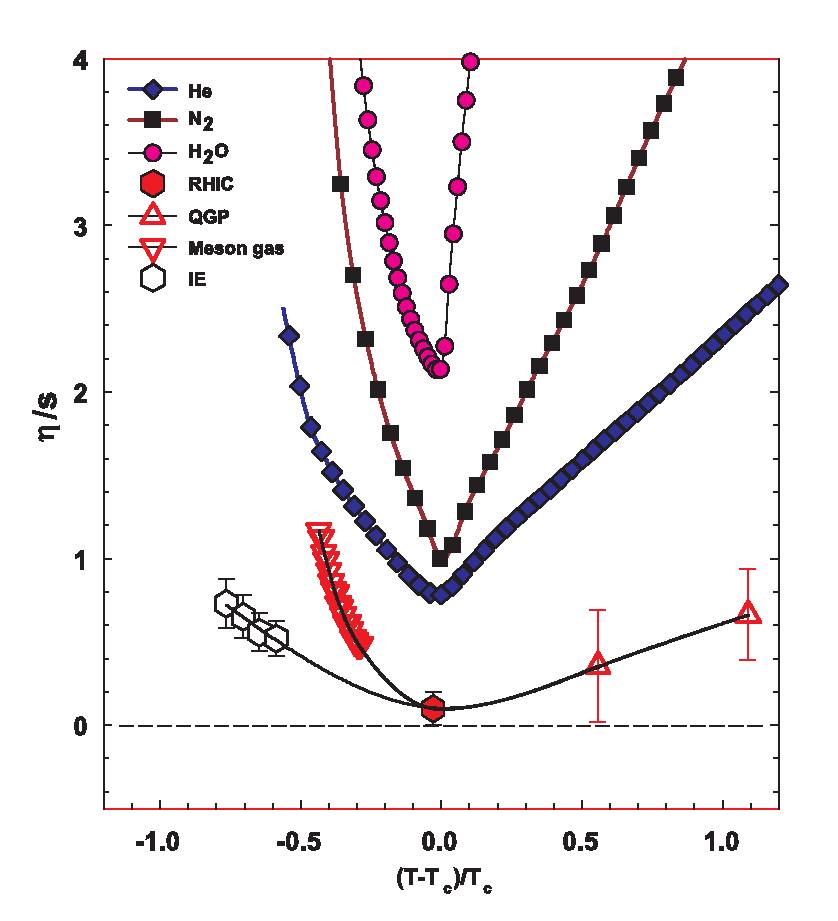
\includegraphics[width=0.9\textwidth]{figures/eta-s-vs-t-tc3}
\caption[$\eta/s$ vs $(T-T_c)/T_c$]{The figure shows \label{fig3}$\eta/s$ as a function of $(T-T_c)/T_c$ for several substances as indicated. The lines are drawn to guide the eye. The $\eta/s=0.09\pm0.015$ value at RHIC is estimated from Au--Au collisions at $\sqrt{s_{NN}}=\unit[200]{\gev}$. The calculations assume a value $T_c = \unit[170]{\mev}$ for nuclear matter. This figure has been reprinted from~\cite{PhysRevLett.98.092301} with kind permission from the American Physical Society.
}%Permission granted
\label{fig:etas}
\end{figure}



\FloatBarrier
\pagebreak
\section{Heavy-ion physics}
Quark Gluon Plasma (QGP) can be experimentally studied by colliding heavy-ions at high energies. Nowadays research of heavy-ion collisions is mainly performed at two particle colliders; The Relativistic Heavy-Ion Collider (RHIC) at BNL in New York, USA and the Large Hadron Collider (LHC) at CERN in Switzerland. Energy densities at these colliders are assumed to be large enough to produce QGP and indeed convincing evidence of QGP has been seen at both colliders. Complimentary research with heavy nuclei is also performed at the Super Proton Synchrotron (SPS) at CERN.

%The history of heavy-ion physics is strongly connected to the development of particle colliders. Experimental study of relativistic heavy-ion collisions has been carried out for three decades, beginning with the Bevalac at Lawrence Berkeley National Laboratory (LBNL)~\cite{Lofgren_1975}, and continuing with the AGS at Brookhaven National Laboratory (BNL)~\cite{Barton:1987}, CERN SPS~\cite{Vitev:2002pf}, culminating today with RHIC at BNL and LHC at CERN. 
%
%%The first colliders could not produce enough energy to create QGP matter so they could only probe the hadronic state. 
%%
%%The collective motion of matter in a heavy-ion collision has been modeled using several models e.g. the Blast wave Model~\cite{PhysRevC.84.064905} has been used succesfully. Another model growing in popularity is the hydrodynamical approach which is further discussed in section \ref{sec:hydro}.
%
%\subsubsection{History}
The first heavy-ion collisions were performed in fixed target experiments at the Bevalac experiment at the Lawrence Berkeley National Laboratory~\cite{Lofgren_1975} and at the Joint Institute for Nuclear Research in Dubna~\cite{kovalenko1994status}, which reached energies of up to \unit[1]{\gev} per nucleon. These were followed in 1986 by the Super Proton Synchrotron (SPS) at CERN which collided oxygen beams with fixed lead targets reaching a centre-of-mass energy per colliding nucleon pair $\left(\sqrt{s_{NN}}\right)$ of \unit[19.4]{\gev}~\cite{Vitev:2002pf}. However, no decisive evidence of QGP was found in these initial experiments. In 1994 SPS introduced a heavier lead beam to produce \PbPb collisions at $\sqrt{s_{NN}}\approx \unit[17]{\gev}$. Simultaneously the Alternating Gradient Synchrotron (AGS) at BNL started colliding ions like $\mathrm{^{32}S}$ with a fixed target at energies of up to \unit[28]{\gev}~\cite{Barton:1987}. In 2000 CERN~\cite{SPSpress} presented compelling evidence for the existence of a new state of matter in SPS. Today SPS is used for fixed-target experiments with \unit[400]{\gev} proton beams. One of these is the SPS heavy-ion and Neutrino Experiment (SHINE)~\cite{Grebieszkow:2013nza}, which tries to search for the critical point of strongly interacting matter.

The next significant addition was the Relativistic Heavy-Ion Collider (RHIC) at BNL in New York, USA which started operating in 2000 and keeps operating to this day. Instead of using fixed targets, RHIC can collide two accelerated beams, significantly increasing the potential centre-of-mass energy. In Au--Au collisions RHIC can reach a centre-of-mass energy per nucleon pair of \unit[200]{\gev}. The experiments at RHIC have provided a lot of convincing evidence that QGP was created~\cite{Adcox:2004mh, Adams:2005dq, Arsene:2004fa, Back:2004je}. 

The newest addition to the group of heavy-ion accelerators is the Large Hadron Collider (LHC) at CERN, Switzerland. Primarily used for proton-proton collisions LHC started operating in November 2009. A year later, in November 2010, first \PbPb heavy-ion runs began at $\sqrt{s_{NN}}=2.76\; \mathrm{TeV}$. Since then LHC has provided both \PbPb and \pPb collisions and a short period of Xe--Xe collisions. Table~\ref{tab:datasets} shows a summary of these. Among the main experiments at LHC, ALICE (a Large Ion Collider Experiment) is dedicated to heavy-ion physics. The all-purpose nature of CMS (Compact Muon Solenoid) and ATLAS (a Toroidal LHC Apparatus) make them well suited also for many heavy-ion studies and they have active heavy-ion programs. The fourth main experiment, LHCb, uses its SMOG system~\cite{Maurice:2017iom} to perform unique fixed target collisions with heavy ions, complementing the other experiments. 


\begin{table}[htb]
\centering
\caption{Summary of datasets. The integrated luminosities are from ALICE.}
\label{tab:datasets}
\begin{tabular}{| c | S | c |}
\hline
\multicolumn{3}{| c |}{Run 1 (2009-2013)} \\
\hline
\multirow{4}{*}{\pp} & 0.90 \tev & $\sim \unit[200]{\mu b^{-1}}$ \\
 & 2.76 \tev & $\sim \unit[100]{n b^{-1}}$ \\
 & 7.00 \tev & $\sim \unit[1.5]{p b^{-1}}$ \\
 & 8.00 \tev & $\sim \unit[2.5]{p b^{-1}}$ \\
 \hline
\pPb & 5.02 \tev & $\sim\unit[15]{n b^{-1}}$ \\
\hline
\PbPb & 2.76 \tev & $\sim \unit[75]{\mu b^{-1}}$ \\
\hline
\end{tabular}
\begin{tabular}{| c | S | c |}
\hline
\multicolumn{3}{| c |}{Run 2 (2015-2018)} \\
\hline
\multirow{2}{*}{\pp} & 5.02 \tev & $\sim \unit[1.3]{p b^{-1}}$ \\
 & 13.00 \tev & $\sim \unit[25]{p b^{-1}}$ \\
 \hline
\multirow{2}{*}{\pPb} & 5.02 \tev & $\sim\unit[3]{n b^{-1}}$ \\
& 8.16 \tev & $\sim\unit[25]{n b^{-1}}$ \\
\hline
Xe--Xe & 5.44 \tev & $\sim \unit[0.3]{\mu b^{-1}}$ \\
\hline
\PbPb & 5.02 \tev & $\sim \unit[1]{n b^{-1}}$ \\
\hline
\end{tabular}
\end{table}

\pagebreak
\FloatBarrier
%\pagebreak
\section{Features of heavy-ion collisions}
\label{sec:features}
\subsection{Collision Geometry}
\label{sec:geometry}
Since atomic nuclei have a significant transverse size, a collision between nuclei has geometric properties that provide insight into the collision dynamics.  One illustration of a heavy-ion collision is shown in Figure~\ref{fig:planes}. The main defining parameter of a collision is the vector connecting the centres of the two colliding nuclei at their closest approach, which is known as the impact parameter $\vec b$.

The impact parameter with the beam direction defines the reaction plane, which has an angle $\Psi_{RP}$ in the experimental reference frame, which is fixed by the detector setup. This reaction plane angle can be estimated with the event plane method~\cite{Voloshin:2008dg} since particle production changes as a function of the angle with respect to the reaction plane. 
\begin{figure}[h!]
\centering
%\definecolor{primary}{HTML}{0000FF}
%\definecolor{secondary}{HTML}{FF8000}
%\definecolor{tertiary}{HTML}{00FFFF}
%\begin{tikzpicture}
%      \draw[->] (-4,0) -- (4,0) node[below] {$x$};
%      \draw[->] (0,-3) -- (0,3) node[left] {$y$};
%       \coordinate[] (C);
% \coordinate[left=1cm of C] (C1);
%\coordinate[right=1cm of C] (C2);
%\draw[dashed, thick, primary] (C1) circle (2cm);
%\draw[dashed, thick, secondary] (C2) circle (2cm);
%      
%\end{tikzpicture}
\documentclass[border=5mm]{standalone}
\usepackage{tikz}
\usetikzlibrary{positioning}
\usetikzlibrary{intersections, calc, fadings}
\begin{document}
\definecolor{primary}{HTML}{0000FF}
\definecolor{secondary}{HTML}{FF8000}
\definecolor{tertiary}{HTML}{00FFFF}


\begin{tikzpicture}[scale=1]
      \draw[->,black!50] (-5.5,0) -- (5.5,0) node[below] {$x$};
      \draw[->,black!50] (0,-4) -- (0,4) node[left] {$y$};
       \coordinate[] (C);
 \coordinate[below left=0.5cm and 1.7cm of C] (C1);
\coordinate[above right=0.5cm and 1.7cm of C] (C2);
\coordinate[below left =1.5cm and 5.1cm of C] (D1);
\coordinate[above right =1.5cm and 5.1cm of C] (D2);

\coordinate[above left =3.4cm and 1.0cm of C] (D3);
\coordinate[below right =3.4cm and 1.0cm of C] (D4);

\draw[->,black!50] (D1) -- (D2) node[above] {$x_\mathrm{RP}$};
\draw[->,black!50] (D4) -- (D3) node[left] {$y_\mathrm{RP}$};

\draw[dashed, thick, primary] (C1) circle (3cm);
\draw[dashed, thick, secondary] (C2) circle (3cm);
\draw[->,thick] (C1) -- node[below right] {$\vec b$} (C2);
\draw[->] (1.5, 0) arc  (0:8.2:1.5cm) node[right] {$\Psi_\mathrm{RP}$} arc (8.2:16.4:1.5cm) ;


\end{tikzpicture}
\end{document}
%\includegraphics[width=0.6\textwidth]{figures/Definitions}
\caption[The definitions of the Reaction Plane coordinate systems]{The definition of the impact parameter and the reaction plane. The $x$--$y$ plane represents a coordinate system fixed by the experiment. The dashed circles are the two colliding nuclei. $x_{RP}$ is the reaction plane and $\Psi_\mathrm{RP}$ gives its angle.} %The angle between $x_{RP}$ and $x_{PP}$ is given by Eq. (\ref{eq:partangle}). $y_{PP}$ and $y_{RP}$ are lines perpendicular to the participant and reaction planes. }
\label{fig:planes}
\end{figure}

Although the length of the impact parameter can be used to quantise the centrality of a heavy-ion collisions in theoretical models, it is not practical in an experimental setup. Any connections between $\vec b$ and experimental observables is model-dependent. For a comparison of results between different experiments and models, one needs a general definition for centrality.

In practice this definition is provided by dividing events into percentile bins by the observed multiplicity of produced particles. In a heavy-ion collision the total multiplicity can be related to the number of participants. Small centrality percentages correspond to central events with the highest multiplicity while peripheral collisions have lower multiplicities and thus higher centrality percentages. Figure~\ref{fig:centrality} shows an observed multiplicity distribution from ALICE measurements~\cite{PhysRevC.88.044909} with the centrality bin division. The distribution is fitted using a phenomenological approach based on a Glauber Monte Carlo calculation~\cite{Miller:2007ri}.

\begin{figure}[tb]
\centering

               \includegraphics[width=0.9\textwidth]{figures/centrality.png}
        \caption[An illustration of the multiplicity distribution in ALICE measurement with centrality classes.]{An illustration of the multiplicity distribution which is divided into centrality bins in ALICE measurements. The red line shows the fit of the Glauber calculation to the measurement. Figure from~\cite{PhysRevC.88.044909}.}
        %Creative commons license
        	\label{fig:centrality}
\end{figure}


The Glauber Model is often used to model the nuclear geometry in a heavy-ion collision. The model was originally introduced already in 1958~\cite{Glauber:1959} and the modern terminology and tools were introduced in 1976 by Białas, Bleszyński, and Czyż~\cite{Biallas1976461} to model inelastic nuclear collisions.


The model starts by defining the thickness function which is the integral of the nuclear density over a line going through the nucleus with minimum distance $s$ from the centre
of the nucleus
\begin{equation}
T_A\left(s\right)=\int_{-\infty}^{\infty}\dd z \rho\left(\sqrt{s^2+z^2}\right),
\end{equation}

\noindent where $ \rho\left(\sqrt{s^2+z^2}\right)$ is the number density of nuclear matter. This can be experimentally determined by studying the nuclear charge distribution in low-energy electron-nucleus scattering experiments~\cite{Miller:2007ri,DeJager:1987qc}. For a spherically symmetric nucleus a good approximation is given by the Woods-Saxon potential~\cite{Abelev:2013qoq}

\begin{equation}
\rho\left( r\right) = \frac{\rho_0 \left(1+\omega r^2 / R^2\right)}{1+\exp \left(\frac{r-R}{a}\right)},
\end{equation}


\noindent where $\rho_0$ is the nucleon density in the centre of the nucleus, $R$ is the nuclear radius, $a$ parametrizes the depth of the skin and $\omega$ can be used to introduce a surface excess. Figure~\ref{fig:woodssaxon} shows how this distribution looks like with parameters observed for lead nuclei. With $\omega=0$ the density changes only slightly as a function of $r$ until it quickly drops to almost 0 around $R$. The slope and length of the transition region is given by $a$. 

\begin{figure}
\centering
\begin{tikzpicture}
      \draw[->] (0,0) -- (7,0) node[below] {$r\left[\unit{fm}\right]$};
      \draw[->] (0,0) -- (0,5) node[left] {$\nicefrac{\rho}{\rho_0}$};
      \draw	(0,0) node[anchor=north] {0}
		(3,0) node[anchor=north] {5}
		(6,0) node[anchor=north] {10};

      \draw	(0,2) node[anchor=east] {0.5}
		(0,4) node[anchor=east] {1};
	
      \draw[dashed,black] (3.8,0) -- (3.8,5);

	
     \draw[black,thin,<->] (0,2) -- node[above] {$R$} (3.8,2);
     \draw[black,thin,<->] (3.55,1) -- node[below] {$a$} (4.05,1);
     
     \draw[blue] (2,3.5) node {$\omega=0$};
     \draw[blue] (2,4.5) node {$\omega>0$};

      \draw[scale=0.6,domain=0:10,smooth,variable=\x,blue,dashed] plot ({\x},{(6.66+1*\x^2/6.38^2)/(1+exp((\x-6.38)/0.546))});
       \draw[scale=0.6,domain=0:10,smooth,variable=\x,blue] plot ({\x},{(6.66)/(1+exp((\x-6.38)/0.546))});

      %\draw[scale=0.5,domain=-3:3,smooth,variable=\y,red]  plot ({\y*\y},{\y});

\end{tikzpicture}
\caption{Woods-saxon distribution, with typical values for a Pb nucleus, $a=0.55\unit{fm}$ and $R=6.6\unit{fm}$.}
\label{fig:woodssaxon}
\end{figure}


The integral over the overlap area of two thickness functions of colliding nuclei defines the overlap function 

\begin{equation}
T_{AB}\left(\vec b\right)=\int \dd{^2s} T_A\left(\vec s\right) T_B\left(\vec s - \vec b\right).
\end{equation}

\noindent In essence this is the material that takes part in the collision for a given impact parameter $\vec b$. The average overlap function, $\left<T_{AA}\right>$, in an A-A collisions  is given by~\cite{Afanasiev:2009aa}

\begin{equation}
\left<T_{AA}\right>=\frac{\int T_{AA}\left(b\right) \dd b}
{\int\left(1-e^{-\sigma^{inel}_{pp}T_{AA}\left(b\right)}\right)\dd b}.
\end{equation}

\noindent Using $\left<T_{AA}\right>$ one can calculate the mean number of binary collisions

\begin{equation}
\left<N_{coll}\right>=\sigma_{pp}^{inel}\left<T_{AA}\right>,
\end{equation}

\noindent where the total inelastic cross-section, $\sigma_{pp}^{inel}$, gives the probability of two individual nucleons interacting. As every binary collision has an equal probability for direct production of high-momentum particles the number of high momentum tracks is proportional to $\left<N_{coll}\right>$~\cite{Abelev:2013qoq,Kharzeev:2004if,Deng:2010mv}. This requires knowledge of $\sigma\mathrm{^{NN}_{inel}}$, which can be measured in proton-proton collisions with different energies. At the LHC the most precise cross section measurements come from TOTEM~\cite{Antchev:2017dia}.

Contrary to hard particles, soft particle production is based on the number of participants~\cite{Kharzeev:2004if}. It can be assumed that participating nucleons get excited and, since the time scales are too short for any reaction to happen in the nucleons, it does not matter how many interactions a single nucleon experiences. After the interactions excited nucleons produce a predictable number of soft particles. The average number of participants, $\left<N_{part}\right>$ can be calculated from the Glauber model  as


\begin{eqnarray}
\left<N_{part}^{AB}\left(\vec b\right)\right>&=&\int \dd{^2s} T_A\left(\vec s\right)\left[1-\left[1-\sigma_{NN}\frac{T_B\left(\vec s - \vec b\right)}{B}\right]^B\right] \nonumber \\
 &+ &\int \dd{^2 s} T_B\left(\vec s\right)\left[1-\left[1-\sigma_{NN}\frac{T_A\left(\vec s - \vec b\right)}{A}\right]^A\right].
\end{eqnarray}



In practice the Glauber model can be implemented in two common ways. Simple analytical expression can be obtained from the optical approximation. These include the nucleus-nucleus interaction cross-section, the number of interacting  nucleons and the number of nucleon-nucleon collisions on average. In the optical Glauber it is assumed that  the nucleons move independently during the crossing of the nuclei and they will be essentially undeflected.  

With increased appreciation for the physics emerging from fluctuations in the collision geometry the Glauber Monte Carlo (GMC) approach has provided a way to get a better  description of heavy-ion collisions. In GMC nucleons are distributed randomly according to the nuclear density distribution~\cite{Abelev:2013qoq}. In the simplest model nucleons of two nuclei will interact if their distance in the orthogonal plane, $d$ is small enough, i.e. 

%A heavy-ion collision is then treated as a series of independent nucleon-nucleon collisions, where in the simplest model nucleons interact if their distance  in the plane orthogonal to the beam axis, $d$, satisfies

\begin{equation}
d< \sqrt{\sigma\mathrm{^{NN}_{inel}}}.
\end{equation}

\noindent The number of participants and binary collisions can be calculated per event.  By simulating many heavy-ion collisions one can then determine both average values and the fluctuation around the average. The results of one GMC \PbPb event with impact parameter $b=\unit[9.8]{fm}$ is shown in Figure~\ref{fig:GMC}.

\begin{figure}[htbp]
\centering
               \includegraphics[width=0.75\textwidth]{figures/test_pbpb_2a}
        \caption[The result of one Glauber Monte Carlo simulation.]{The figure shows a \PbPb collision in a Glauber Monte Carlo simulation. The big circles with black dotted boundaries outline the two colliding nuclei. Small blue and red circles represent nucleons with different colours for the two nuclei. Circles with solid boundaries are participants i.e. there is an overlap with at least one nucleon from the other nucleus. Circles with dotted boundaries are spectators which do not take part in the collision~\cite{Alver:2008aq}.}
        %Permission needed?
        	\label{fig:GMC}
\end{figure}



\subsection{Collective motion}
\label{sec:collective}
For most cases the evolution of a heavy-ion event can be separated into four stages. A schematic illustration of the evolution of a heavy-ion collision with this division is shown in Figure~\ref{fig:HISpaceTime}. Stage 1 is the pre-equilibrium stage, the phase immediately after the collision. It is commonly assumed to last about $1\ \mathrm{fm}/c$ in proper time $\tau$. 
%Hydrodynamic description is not applicable to this regime because thermal equilibrium is not yet reached. 

\begin{figure}[htb]
\centering
               \includegraphics[width=0.75\textwidth]{figures/HISpaceTime2}
        \caption[Schematic representation of a heavy-ion collision]{Schematic representation of a heavy-ion collision as a function of time and the longitudinal coordinate $z$. The various stages of the evolution are separated by hyperbolic curves which are defined by fixed proper time $\tau=\sqrt{t^2-z^2}$. Figure from~\cite{Romatschke:2009im}.}
        %Creative commons
        	\label{fig:HISpaceTime}
\end{figure}

During the second stage the system has thermal equilibrium or at least a near-equilibrium. This lasts about $5-10\ \mathrm{fm}/c$ until the temperature of the system decreases enough for the system to lose its deconfined, strongly coupled state and hadronisation occurs. During stage 2 the matter is driven outwards by the large pressure gradient from the centre of the collision to the vacuum outside the collision volume. 

During stage 3 the hadrons still interact with each other. This ends when hadron scattering becomes rare and in the final phase hadrons become free streaming until they reach the detector.

In a heavy-ion collision the bulk collective particle production that is emitted from the QGP medium is referred to as flow. During hadronisation the pressure-driven expansion of QGP turns into the flow of mainly low-momentum particles. Since the expansion is close to isotropic the resulting particle flow is isotropic with small anisotropies of the order of $10\%$ at most. The isotropic component of flow is referred to as radial flow. Figure~\ref{fig:dndpt} shows the transverse momentum spectra $\dd N/\dd {\pt{}}$ in heavy-ion collisions. 

%In this stage hydrodynamics should be applicable if the temperature is above the deconfinement temperature~\cite{Romatschke:2009im}. 
% strongly coupled, state and hydrodynamics can no longer be used.






\begin{figure}[b!]
\centering
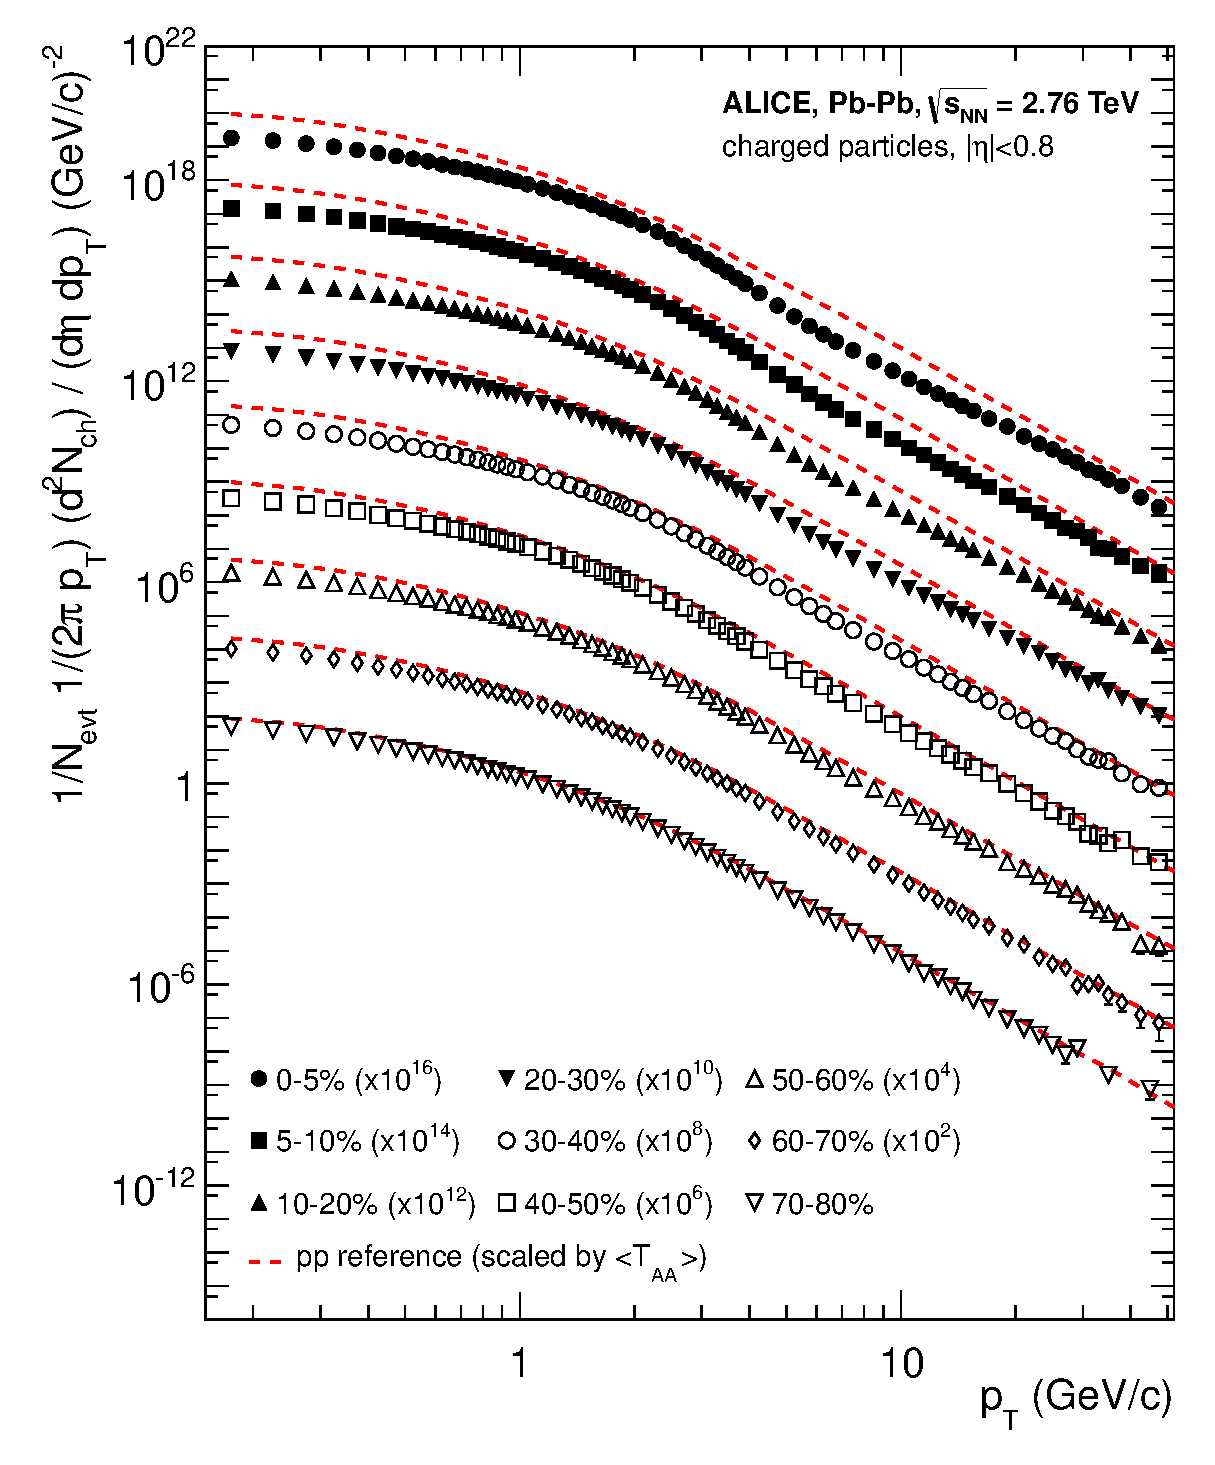
\includegraphics[width=0.6\textwidth]{figures/pT_PbPb}
\caption[Charged particle spectra]{The radial flow is represented by the charged particle spectra for different centrality classes given in the legend. The dashed lines show  proton-proton reference spectra which are scaled by the nuclear overlap function determined for each centrality class.  For clarity the distributions and the reference spectra are offset by arbitrary factors. Figure from~\cite{PRL106032301}.}
%Creative commons license
\label{fig:dndpt}
\end{figure}

%Figure~\ref{fig:dndpt} shows the transverse momentum spectra $\dd N/\dd {\pt{}}$ in heavy-ion collisions. As the vast majority of produced particles have small $\pt{}$, any observables that are integrated over $\pt{}$ are dominated by the small momentum region of the spectrum. The difference between the yield of $\unit[1]{\GeVc}$ and $\unit[4]{\GeVc}$ particles is already 2-3 orders of magnitude.

The geometry of the heavy-ion collision produces an anisotropic component to the collective motion. Figure~\ref{fig:flow} gives illustrations of collisions with different impact parameters. In a non-central heavy-ion collision, with a large impact parameter, the impact zone has an elliptical shape in the transverse plane. In a central collision, with a small impact parameter, the overlap region is almost circular.

\begin{figure}[b!]
\centering
        \begin{subfigure}[b]{0.52\textwidth}
                \centering
	         \includegraphics[height=2.4in]{figures/tikz/central}

                \caption{Peripheral collision}
                \label{fig:InteractionB}
        \end{subfigure}
        \begin{subfigure}[b]{0.45\textwidth}
                \centering
                \includegraphics[height=2.4in]{figures/tikz/peripheral}

                \caption{Central collision}
                \label{fig:InteractionA}
        \end{subfigure}
	\caption[Illustration of flow in momentum space in central and peripheral collisions.]{Illustration of elliptic flow in central and peripheral collisions. The density of the arrows represent the strength of flow in the corresponding azimuthal direction as seen in the detectors. In a peripheral collision momentum the difference in pressure gradients gives a strong flow into the in-plane direction while the flow into the out-of-plane direction is small. In a central collision flow is more isotropic and dominated by higher harmonics. In the figure the difference is exaggerated and the difference in total multiplicity is not taken into account.}
	\label{fig:flow}
\end{figure}

During the evolution of the QGP medium this asymmetry of the impact zone is transformed into the asymmetry of particle production in momentum space. The distance from high pressure, the collision centre to low pressure, vacuum outside the impact zone varies. It is smallest in the direction of the impact parameter $\vec b$ and thus the pressure gradient is strongest in this direction, in-plane. The higher pressure gradient will produce more collective flow as compared to the out-of-plane direction~\cite{Ollitrault:1992,Ollitrault:1993, Heinz:2002}. Figure~\ref{fig:flow} illustrates the difference in impact zone and resulting flow.


Flow anisotropy is typically parametrised in the form of a Fourier composition 

\begin{equation}
E\frac{\dd{^3N}}{\dd {p^3}}=\frac{1}{2\pi}\frac{\dd {^2N}}{\pt{ }\dd {\pt{ }}\dd {\eta} } \left(1+\sum_{n=1}^{\infty}2v_n\left(\pt{},\eta\right)\cos(n(\phi-\Psi_n))\right),
%\label{eq:finalseries}
\end{equation}

\noindent where the overall normalisation, $\frac{1}{2\pi}\frac{\dd {^2N}}{\pt{ }\dd {\pt{ }}\dd {\eta} }$, gives the strength of radial flow, $\Psi_n$ gives the rotation angle of the component $n$ contribution, and the coefficients $v_n$ give the relative contributions of anisotropic flow components. The coefficients can depend on both transverse momentum $\pt{}$ and pseudorapidy $\eta$. As in general Fourier analysis is known as harmonic analysis the components are often referred to as harmonic flow components. 
Elliptic flow, i.e. flow with two maxima, is represented by $v_2$ and $v_3$ represents triangular flow while the first coefficient, $v_1$, is connected to directed flow~\cite{Voloshin:1994mz}. Because of momentum conservation directed flow is in total assumed to be zero. In certain rapidity or momentum regions it can be nonzero but it must be canceled by other regions.

In a peripheral collision $v_2$ is the dominant part of anisotropic flow as it arises from the asymmetric geometry of the collision region.  For a long time the odd harmonics were considered to be negligible, because they would require a more complex asymmetry. In 2007 Mishra {\emph et al.}~\cite{Mishra:2007tw} argued that inhomogeneities in the initial state density would lead to non-zero $v_n$ values for $v_3$ and other higher harmonics. As the colliding nuclei are not static objects, the arrangement of the nucleons at the time of a collision is random~\cite{Alver:2010gr}. Therefore the shape of the collision zone is not symmetric but rather more complex. On the other hand, inside the collision zone the created medium is not homogenous. Instead the medium includes hot spots with higher density. It is expected that higher harmonics of $v_n$ would be suppressed more by viscous effects and thus the shape of $v_n$ as a function of $n$ could be used to study $\eta/s$~\cite{Mocsy:2010um}.

The first one to predict anisotropic flow in heavy-ion collisions was Ollitrault in 1992~\cite{Ollitrault:1992} and the first experimental studies were conducted in 1993 at the AGS~\cite{PhysRevLett.70.1393}. Instead of the Fourier composition these initial studies used alternative approaches. In AGS the reaction plane angle in one rapidity region was observed to be correlated with the particle production in another rapidity region. The first ones to introduce the Fourier decomposition were Voloshin and Zhang in 1996~\cite{Voloshin:1994mz}.


\begin{figure}[tb]
	\centering
	\begin{subfigure}[t]{0.5\textwidth}
                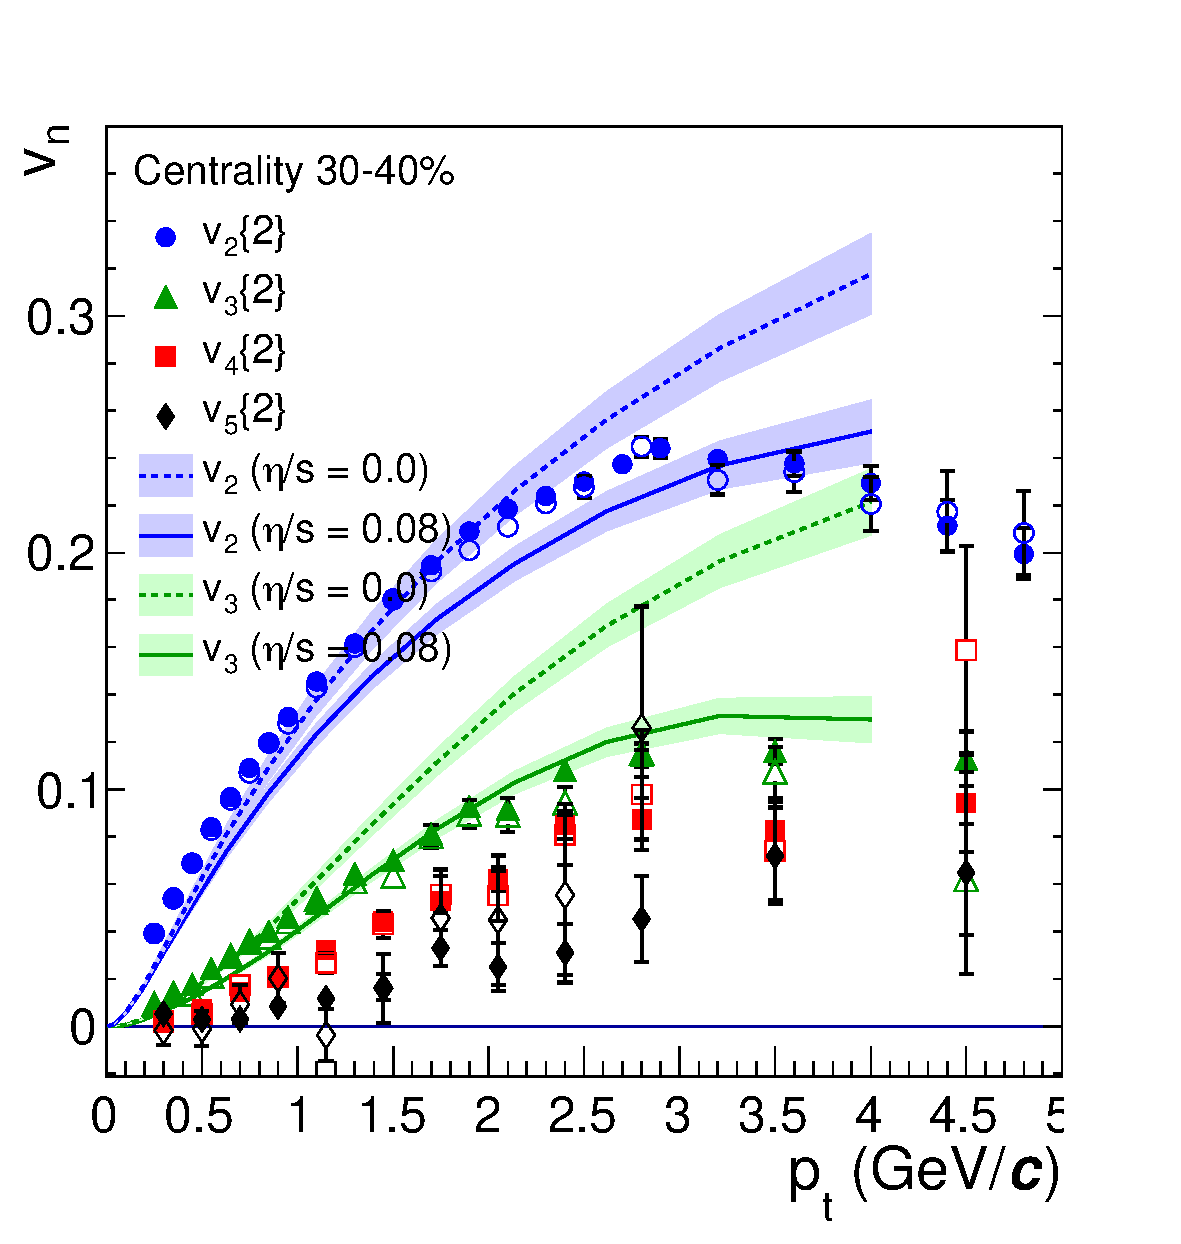
\includegraphics[width=\textwidth]{figures/alice_vn_figa.pdf}
        %\caption[ALICE measurement of $v_2$, $v_3$, $v_4$, $v_5$]{ALICE measurement of $v_2$, $v_3$, $v_4$, $v_5$ as a function of transverse momentum. The flow coefficients are determined by two-particle correlations using different rapidity separations.  The full and open symbols are for $\Delta\eta > 0.2$ and $\Delta\eta > 1.0$. The results are compared to hydrodynamic predictions~\cite{Schenke:2011tv} with different values of $\eta/s$~\cite{PRL107032301}.}
        \label{fig:higherharmonics}
        \end{subfigure}
        \quad
        \begin{subfigure}[t]{0.45\textwidth}
        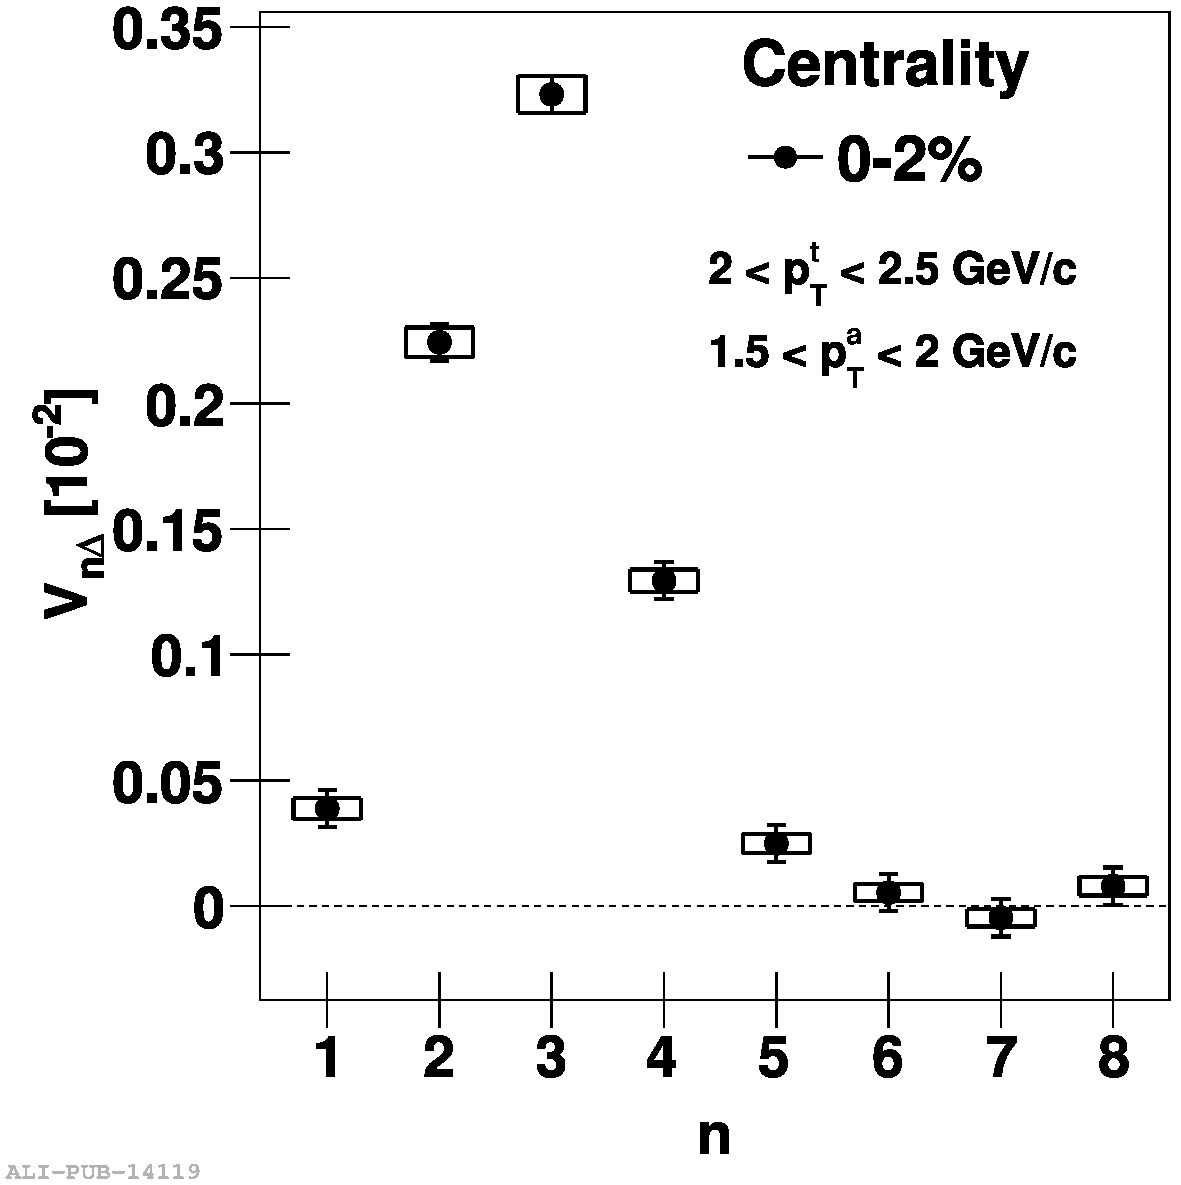
\includegraphics[width=\textwidth]{figures/2012-Jun-06-fig02b}
       % \caption{Amplitude of $v_n$ harmonics as a function of $n$ for the 2\% most central collisions as  measured by ALICE~\cite{Aamodt2012249}.}
        \label{fig:alicepowers}

        \end{subfigure} 
        
%        \begin{subfigure}[t]{\textwidth}
 %               \includegraphics[width=\textwidth]{figures/atlas_powerspectra.png}
%        \caption{Power spectra of $v_n$ for the 1\% most central collisions measured by ATLAS~\cite{PhysRevC.86.014907}.}
%        \label{fig:atlaspowers}
 %       \end{subfigure}
                \caption[Flow measurements of higher harmonics]{Flow measurements of higher harmonics. \emph{left:} ALICE measurement of $v_2$, $v_3$, $v_4$, $v_5$ as a function of transverse momentum. Two-particle correlations are used to obtain the harmonic coefficients. The full and open symbols are for different $\Delta\eta$ separation between the particles ($\Delta\eta > 0.2$ and $\Delta\eta > 1.0$). The observations are compared to hydrodynamic calculations~\cite{Schenke:2011tv} with varying values of the shear viscosity to entropy ratio $\eta/s$. Figure from~\cite{PRL107032301}. \emph{right:} Amplitude of $v_n$ coefficients as a function of $n$ for the 2\% most central collisions as measured by ALICE. Figure from~\cite{Aamodt2012249}. }
                %Creative commons license
                \label{fig:vnpowers}

\end{figure}


Figure~\ref{fig:vnpowers} shows measurements of different harmonics coefficients. The left panel shows the flow coefficients in peripheral collisions as a function of track $\pt{}$ as measured by ALICE~\cite{PRL107032301}.  As shown on the right hand panel of Figure~\ref{fig:vnpowers} the $v_n$ values decrease in central collisions as a function of $n$ for $n>3$. In peripheral collisions the elliptic flow component $v_2$ will be larger.

In Figure~\ref{fig:vnpowers} the results are compared to predictions from hydrodynamic calculations~\cite{Schenke:2011tv}. In general the measured collective flow in heavy-ion collisions has been successfully modelled with the relativistic version of hydrodynamics. The power of this approach lies in its simplicity and generality. Hydrodynamic calculations only require that the system reaches at least local thermal equilibrium. For this the system must have a mean free path that is shorter than the length scales of interest, which is assumed to hold for the strongly coupled QGP phase of a heavy-ion collision~\cite{Romatschke:2009im}.

The first approaches using the relativistic version of hydrodynamics were performed already in the 1950's~\cite{Landau:1953gs}, before QCD was discovered. The early studies used it to model proton-proton collisions. For the use of heavy-ion collisions hydrodynamics has been under development since the 1980's. One early example is the study of boost-invariant longitudinal expansion and infinite transverse flow by Bjorken~\cite{PhysRevD.27.140}. Later studies added finite size and dynamically generated transverse size~\cite{Baym:1984sr, PhysRevD.34.794}. 

%Major steps were taken later with the addition of finite size and and dynamically generated transverse size~\cite{Baym:1984sr, PhysRevD.34.794}, a part of which was done at the University of Jyväskylä. %The role of hydrodynamics in heavy-ion physics was strengthened when QGP was observed to behave like a liquid by RHIC~\cite{Adcox:2004mh}. 

Over the years understanding of the properties of the QGP has been improved with the help of new data from LHC and RHIC and theoretical developments.
For example, as shown in Figure~\ref{fig:etasT}(a), the quantification of the temperature dependence of the shear viscosity over entropy ratio, $\eta/s$ has been tested with an event-by-event model~\cite{Niemi:2015qia} that combines viscous hydrodynamic calculations with the Eskola-Kajantie-Ruuskanen-Tuominen (EKRT) model for initial conditions.
%event-by-event Eskola-Kajantie-Ruuskanen-Tuominen (EKRT) + viscous hydrodynamic calculations~\cite{Niemi:2015qia}, where the first qualitative possibilities of the dependence were investigated.

The initial density profiles for hydrodynamic simulations are calculated using a next-to-leading order perturbative-QCD (pQCD) and the EKRT model~\cite{Paatelainen:2012at,Paatelainen:2013eea}. The following space-time evolution is described by relativistic dissipative fluid dynamics. The simulation is performed using different parametrisations of the temperature dependence of the shear viscosity to entropy density ratio $\eta/s(T)$. 

This model has been observed to give a good description of the charged hadron multiplicity and of the low-\pt{} region of the charged hadron spectra both at RHIC and at LHC~\cite{Niemi:2015qia}. Each of the different $\eta/s(T)$ parametrisations were adjusted to reproduce the measured $v_n$ from central to mid-peripheral collisions.
Previous measurements~\cite{ALICE:2016kpq} have ruled out models where the temperature of the phase transition is larger than for "param1".
The two sets of parameters which described most of the data are labeled as "best fits" in Figure~\ref{fig:etasT}(a).
For the "param1" parametrisation the phase transition from the hadronic to the QGP phase occurs at the lowest temperature, around 150~MeV. This parametrisation is also characterised by a moderate slope in $\eta/s(T)$ which decreases (increases) in the hadronic (QGP) phase.

The estimation of the $\eta/s(T)$ dependence has been also studied with a Bayesian analysis, which is applied to form the initial conditions with no assumptions on the physical mechanisms of entropy production~\cite{Bernhard:2016bar}. The robust statistical analytical methods allow calibrating the model to data in a multi-dimensional parameter space. In addition to finding the most likely combination of input parameters, the Bayesian statistical method provides the full uncertainty quantification in the form of posterior probability distributions for all the parameters. The $\eta/s(T)$ parametrisation resulting from this analysis is shown in Figure~\ref{fig:etasT}(b).

\begin{figure}
       \begin{overpic}[width=0.45\textwidth]{figures/etapers_bestfit.pdf}
         \put(10,82){\tiny H. Niemi, K.J. Eskola, R.Paatelainen}
         \put(10,78){\tiny (Phys. Rev. C 93, 024907 (2016), arXiv:1505.02677)}
        \end{overpic}
        \begin{overpic}[width=0.55\textwidth]{figures/region_shear.pdf}
         \put(9,70){\tiny Steffen A. Bass et. al, Global Bayesian Analysis}
          \put(9,67){\tiny (Nucl.Phys. A967 (2017) 67-73 , arXiv:1704.07671)}
          \put(15,35){\small(b)}
        \end{overpic}
        \caption{Temperature dependence of $\eta/s$. \emph{left:} Different parametrisations of $\eta/s(T)$ that have been tested in hydrodynamical simulations. \emph{right:}  Result of a global Bayesian analysis narrowing down the possible $\eta/s(T)$ behaviour. These figures have been reprinted from ~\cite{Niemi:2015qia} and ~\cite{Bernhard:2016bar} with kind permissions from the American Physical Society.}
        \label{fig:etasT}
        '%Permission asked for a) and b)
 \end{figure}

Based on these model calculations, the phase transition from the hadronic to the QGP phase occurs at the lowest temperature, around 150~MeV.
Although the temperature dependence of the $\eta/s$ is still not well established, the calculations generally suggest a minimum value of $\eta/s$~from 0.08 to 0.12, close to the universal limit $1/(4\pi)$~\cite{Kovtun:2004de}.

Recently, several advancements have been made in order to further constrain the temperature dependence of $\eta/s$. New observables, such as the symmetric cumulants~\cite{ALICE:2016kpq,Acharya:2017gsw}, have provided detailed information on the temperature dependence over the evolution of the QGP. Furthermore, the non-linear formalism has resulted in remarkable new constraints on the initial conditions~\cite{Acharya:2017zfg}, and the $\eta/s$ at the freeze-out conditions, which is among the least understood parts of hydrodynamic calculations.


%Comparing hydrodynamical calculations to experimental results has provided a path to studying the $\eta/s$ value of QGP. 













% !TEX root = thesis.tex

\section{Hard processes}
\subsection{pQCD factorization}


%\begin{figure}[htb]
%\centering
%\includegraphics[width=0.5\textwidth]{pics/QCDLO}
%\caption[QCD Leading Order]{The basic pQCD processes and their quadratic matrix elements}
%\label{fig:qcdlo2}
%\end{figure}





The term Hard Scattering is used for the scattering of two point-like constituents (partons) of colliding nucleons, when the momentum transfer $Q^2$ is large ($Q \gg \Lambda_{\mathrm{QCD}}$). Figure ~\ref{fig:scattering} shows the incoming partons, quarks or gluons, as they exchange a space-like virtual gluon and produce two highly virtual outgoing partons. The outgoing partons will eventually fragment into collimated showers of partons, referred to as jets.

\begin{figure}[htb]
\centering
\documentclass{standalone}
\usepackage{tikz}
\usepackage{xcolor}
\usetikzlibrary{shapes,arrows}
\usetikzlibrary{trees}
\usetikzlibrary{shadows.blur}
\usetikzlibrary{positioning}
\usetikzlibrary{decorations.pathmorphing}
\usetikzlibrary{decorations.markings}
\begin{document}

\tikzset{
photon/.style={decorate, decoration={snake}, draw=red},
particlearrow/.style={draw=blue, postaction={decorate},
    decoration={markings,mark=at position .5 with {\arrow[draw=black]{>}}}},
antiparticlearrow/.style={draw=blue, postaction={decorate},
    decoration={markings,mark=at position .5 with {\arrow[draw=black]{>}}}},
particle/.style={draw=blue},
antiparticle/.style={draw=blue},
gluon/.style={decorate, draw=magenta,
    decoration={coil,amplitude=4pt, segment length=5pt}}
 }
 
 
 
\tikzstyle{proton} = [ellipse, draw=black, text centered, fill=red!20, minimum height=3em, blur shadow = {shadow blur steps=5},minimum width=1em ] 
\begin{tikzpicture}[node distance=1cm and 1.5cm]
\coordinate[] (p1);
\node[proton, right of=p1]  (proton)  {};
\coordinate[below right=-0.05cm and 0.02cm of proton] (aux1);
\coordinate[above right=-0.05cm and 0.02cm of proton] (aux2);
\coordinate[below right=0.0cm and 2cm of aux1] (vertex1);
\coordinate[right=2cm of aux2] (aux4);
\coordinate[right=2cm of proton] (aux5);
\coordinate[right=2cm of aux4] (spec1);
\coordinate[right=2cm of aux5] (spec2);

\coordinate[below right=1.5cm and 0.5cm of vertex1] (vertex2);

\coordinate[below right=0.0cm and 2cm of vertex2] (b1);
\node[proton, below right=-0.05cm and 0.02cm of b1] (proton2) {};
\coordinate[left=2cm of proton2] (aux6);
\coordinate[below left=-0.05cm and 0.02cm of proton2] (b2);
\coordinate[left=2cm of b2] (aux7);
\coordinate[left=2cm of aux7] (spec3);
\coordinate[left=2cm of aux6] (spec4);
\coordinate[right of=proton2] (p2);
\coordinate[above right=1cm and 1cm of vertex1] (jet1);
\coordinate[below left=1cm and 1cm of vertex2] (jet2);


%Jet cones
\coordinate[above right=1cm and 0.5cm of jet1] (cone11);
\coordinate[above right=0.5cm and 1cm of jet1, label={right:Jet}] (cone12);
\draw[particle] (jet1) -- (cone11);
\draw[particle] (jet1) -- (cone12);
\draw[blue] (cone11) to[out=45,in=45]  (cone12);
\draw[blue] (cone11) to[out=225,in=225] (cone12);

\coordinate[below left=1cm and 0.5cm of jet2] (cone21);
\coordinate[below left=0.5cm and 1cm of jet2, label={left:Jet}] (cone22);
\draw[particle] (jet2) -- (cone21);
\draw[particle] (jet2) -- (cone22);
\draw[blue] (cone21) to[out=45,in=45]  (cone22);
\draw[blue] (cone21) to[out=225,in=225] (cone22);

\draw[particlearrow] (p1) -- node[label=above:$P_A$] {} (proton); 
\draw[particlearrow] (aux1) -- node[label=below:$x_a$] {} (vertex1); 
\draw[particlearrow] (aux2) -- (aux4); 
\draw[particlearrow] (proton) -- (aux5);
\draw[particle] (aux4) -- (spec1);
\draw[particle] (aux5) -- (spec2);
\draw[particle] (aux7) -- (spec3);
\draw[particle] (aux6) -- (spec4);
\draw[particle] (vertex1) -- (jet1);
\draw[particle] (vertex2) -- (jet2);

\draw[gluon] (vertex1) -- node[label=right:$q$] {} (vertex2);
\draw[particlearrow] (b1) -- node[label=above:$x_b$] {} (vertex2);
\draw[particlearrow] (b2) -- (aux7);
\draw[particlearrow] (proton2) -- (aux6);

\draw[particlearrow] (p2) -- node[label=above:$P_B$] {} (proton2);




\end{tikzpicture}



\end{document}

%\includegraphics[width=0.5\textwidth]{pics/ink}
\caption[Hard scattering]{Schematic view of hard scattering process between two protons, producing two jets}
\label{fig:scattering}
\end{figure}

Historically one would study hard scatterings foremost with inclusive hadron spectra. In this context hadron production from hard scatterings can be factorised into three components; the parton distribution functions $f_a$, $f_b$ that give the probability of getting a parton with momentum fraction $x$ of the proton, the cross section of the elementary scattering $ab\rightarrow cd$,  and the fragmentation functions, $D_{h/c}^0$, that give the probability of getting hadron $h$ from the parton.

\begin{equation}
\frac{\mathrm{d} \sigma^h_{pp}}{\mathrm{d}y\mathrm{d}^2\pt{}} = K \Sigma_{abcd}\int \mathrm{d}x_a \mathrm{d}x_b f_a\left(x_a,Q^2\right) f_b\left(x_b, Q^2\right) \frac{\mathrm{d} \sigma}{\mathrm{d}t}\left(ab\rightarrow cd \right)\frac{D_{h/c}^0}{\pi z_c},
\end{equation}

\noindent where $K$ is normalisation constant and

\begin{equation}
x_{a,b} = \frac{\left| p_{a,b} \right|}{\left| p_{proton} \right|}.
\end{equation}


Parton distribution functions will be discussed further in the following section. The elementary cross section $ab\rightarrow cd$ can be calculated from QCD. A summary of the first order $2\rightarrow2$ processes in QCD is shown in Figure ~\ref{fig:qcdlo}. 

The final component in the factorization, fragmentation functions, describe the distribution of the fractional momenta of fragments radiated from the outgoing parton.  In a leading order picture, it can be interpreted as the probability that the observed final state originates from a given parton~\cite{Metz:2016swz}. Like the PDFs they are non-perturbative and must be determined experimentally. Most measurements come from $e^+ e^-$ collisions where the kinematics are better controlled. 


%
%\begin{figure}
%\centering
%\includegraphics[width=0.9\textwidth]{pics/Showering}
%\caption[Jet showering]{REPLACE FIGURE An illustration of jet showering. The highly virtual parton from the hard scattering will produce a shower of softer partons. When the virtuality is low enough the shower will go through a hadronisation process that produces the hadrons, which will be eventually observed in the detector. }
%\label{fig:highpt}
%\end{figure}



\begin{figure}[tb]
\centering
\documentclass{standalone}
\usepackage{tikz}
\usepackage{array}
\usetikzlibrary{shapes,arrows}
\usetikzlibrary{trees}
\usetikzlibrary{shadows.blur}
\usetikzlibrary{positioning}
\usetikzlibrary{decorations.pathmorphing}
\usetikzlibrary{decorations.markings}
\begin{document}
\newcommand{\centered}[1]{\begin{tabular}{l} #1 \end{tabular}}

\tikzset{
photon/.style={decorate, decoration={snake}, draw=red},
particlearrow/.style={draw=black, postaction={decorate},
    decoration={markings,mark=at position .5 with {\arrow[draw=black]{>}}}},
antiparticlearrow/.style={draw=black, postaction={decorate},
    decoration={markings,mark=at position .5 with {\arrow[draw=black]{>}}}},
particle/.style={draw=black},
antiparticle/.style={draw=blue},
gluon/.style={decorate, draw=black,
    decoration={coil,amplitude=2pt, segment length=3pt}}
 }
 
%\begin{tabular}{ >{\centering\arraybackslash} m{2cm} >{\centering\arraybackslash} m{2cm} >{\centering\arraybackslash} m{8cm}}
\begin{tabular}{ c c c}

\begin{tabular}{c}
$qq' \rightarrow qq' $ \\
$\bar q q' \rightarrow \bar qq' $
\end{tabular} 
& $\frac{4}{9}\frac{\hat s^2+\hat u^2}{\hat t^2}$

&
\centered{

 \begin{tikzpicture}[node distance=1cm and 1.5cm]
\coordinate[] (e1);
\coordinate[right=1cm of e1] (aux1);
\coordinate[right=1cm of aux1] (e2);
\coordinate[below=1cm of aux1] (aux2);
\coordinate[left=1cm of aux2] (e3);
\coordinate[right=1cm of aux2] (e4);

\draw[particle] (e1) -- (aux1);
\draw[particle] (aux1) -- (e2);
\draw[particle] (e3) -- (aux2);
\draw[particle] (aux2) -- (e4);
\draw[gluon] (aux2) -- node[label=left:$t$] {} (aux1);
\end{tikzpicture} 

}
 \\
$qq \rightarrow qq$ & $\frac{4}{9}\left( \frac{\hat s^2+\hat u^2}{\hat t^2} + \frac{\hat s^2+\hat u^2}{\hat t^2}  \right) - \frac{8}{27}\frac{\hat s^2}{\hat u \hat t}$ &
\centered{

\begin{tikzpicture}[node distance=1cm and 1.5cm]
\coordinate[] (e1);
\coordinate[right=1cm of e1] (aux1);
\coordinate[right=1cm of aux1] (e2);
\coordinate[below=1cm of aux1] (aux2);
\coordinate[left=1cm of aux2] (e3);
\coordinate[right=1cm of aux2] (e4);

\draw[particlearrow] (e1) -- (aux1);
\draw[particlearrow] (aux1) -- (e2);
\draw[particlearrow] (e3) -- (aux2);
\draw[particlearrow] (aux2) -- (e4);
\draw[gluon] (aux2) -- node[label=left:$t$] {} (aux1);
\end{tikzpicture} 

\begin{tikzpicture}[node distance=1cm and 1.5cm]
\coordinate[] (e1);
\coordinate[right=1cm of e1] (aux1);
\coordinate[right=1cm of aux1] (e2);
\coordinate[below=1cm of aux1] (aux2);
\coordinate[left=1cm of aux2] (e3);
\coordinate[right=1cm of aux2] (e4);

\draw[particlearrow] (e1) -- (aux1);
\draw[particle] (aux1) -- (e4);
\draw[particlearrow] (e3) -- (aux2);
\draw[particle] (aux2) -- (e2);
\draw[gluon] (aux2) -- node[label=left:$u$] {} (aux1);
\end{tikzpicture}
}
\\
$\bar q q \rightarrow \bar q' q'$ & $\frac{4}{9}\frac{\hat t^2+\hat u^2}{\hat s^2}$ &
\centered{
\begin{tikzpicture}[node distance=1cm and 1.5cm]
\coordinate[] (e1);
\coordinate[below right=0.7cm of e1] (aux1);
\coordinate[right=1cm of aux1] (aux2);
\coordinate[above right=0.7cm of aux2] (e2);
\coordinate[below left=0.7cm of aux1] (e3);
\coordinate[below right=0.7cm of aux2] (e4);

\draw[antiparticlearrow] (aux1) -- (e1);
\draw[antiparticlearrow] (e2) -- (aux2);
\draw[particlearrow] (e3) -- (aux1);
\draw[particlearrow] (aux2) -- (e4);
\draw[gluon] (aux2) -- node[label=above:$s$] {} (aux1);
\end{tikzpicture}
}
\\
$\bar q q \rightarrow \bar q q$ & $\frac{4}{9}\left( \frac{\hat s^2+\hat u^2}{\hat t^2} + \frac{\hat t^2+\hat u^2}{\hat s^2}  \right) - \frac{8}{27}\frac{\hat u^2}{\hat s \hat t}$ &
\centered{

\begin{tikzpicture}[node distance=1cm and 1.5cm]
\coordinate[] (e1);
\coordinate[below right=0.7cm of e1] (aux1);
\coordinate[right=1cm of aux1] (aux2);
\coordinate[above right=0.7cm of aux2] (e2);
\coordinate[below left=0.7cm of aux1] (e3);
\coordinate[below right=0.7cm of aux2] (e4);

\draw[antiparticlearrow] (aux1) -- (e1);
\draw[antiparticlearrow] (e2) -- (aux2);
\draw[particlearrow] (e3) -- (aux1);
\draw[particlearrow] (aux2) -- (e4);
\draw[gluon] (aux2) -- node[label=above:$s$] {} (aux1);
\end{tikzpicture}
\begin{tikzpicture}[node distance=1cm and 1.5cm]
\coordinate[] (e1);
\coordinate[right=1cm of e1] (aux1);
\coordinate[right=1cm of aux1] (e2);
\coordinate[below=1cm of aux1] (aux2);
\coordinate[left=1cm of aux2] (e3);
\coordinate[right=1cm of aux2] (e4);

\draw[antiparticlearrow] (e2) -- (aux1);
\draw[antiparticlearrow] (aux1) -- (e1);
\draw[particlearrow] (e3) -- (aux2);
\draw[particlearrow] (aux2) -- (e4);
\draw[gluon] (aux2) -- node[label=left:$t$] {} (aux1);
\end{tikzpicture} 
}
\\
$\bar q q \rightarrow gg$ & $\frac{32}{27}\frac{\hat u^2+\hat t^2}{\hat u \hat t} - \frac{8}{3}\frac{\hat u^2 + \hat t^2}{\hat s^2}$ &
\centered{

\begin{tikzpicture}
\coordinate[] (e1);
\coordinate[below right=0.7cm of e1] (aux1);
\coordinate[right=1cm of aux1] (aux2);
\coordinate[above right=0.7cm of aux2] (e2);
\coordinate[below left=0.7cm of aux1] (e3);
\coordinate[below right=0.7cm of aux2] (e4);

\draw[antiparticlearrow] (aux1) -- (e1);
\draw[gluon] (aux2) -- (e2);
\draw[particlearrow] (e3) -- (aux1);
\draw[gluon] (aux2) -- (e4);
\draw[gluon] (aux2) -- node[label=above:$s$] {} (aux1);
\end{tikzpicture}
}
\\
$gg \rightarrow \bar q q$ & $\frac{1}{6}\frac{\hat u^2+\hat t^2}{\hat u \hat t} - \frac{3}{8}\frac{\hat u^2 + \hat t^2}{\hat s^2}$ &
\centered{

\begin{tikzpicture}
\coordinate[] (e1);
\coordinate[below right=0.7cm of e1] (aux1);
\coordinate[right=1cm of aux1] (aux2);
\coordinate[above right=0.7cm of aux2] (e2);
\coordinate[below left=0.7cm of aux1] (e3);
\coordinate[below right=0.7cm of aux2] (e4);

\draw[gluon] (e1) -- (aux1);
\draw[antiparticlearrow] (e2) -- (aux2);
\draw[gluon] (e3) -- (aux1);
\draw[particlearrow] (aux2) -- (e4);
\draw[gluon] (aux2) -- node[label=above:$s$] {} (aux1);
\end{tikzpicture}
}
\\

$q g  \rightarrow qg $ & $\frac{4}{9}\frac{\hat u^2+\hat s^2}{\hat u \hat s} + \frac{\hat u^2 + \hat s^2}{\hat t^2}$ &
\centered{

\begin{tikzpicture}
\coordinate[] (e1);
\coordinate[below right=0.7cm of e1] (aux1);
\coordinate[right=1cm of aux1] (aux2);
\coordinate[above right=0.7cm of aux2] (e2);
\coordinate[below left=0.7cm of aux1] (e3);
\coordinate[below right=0.7cm of aux2] (e4);

\draw[gluon] (e1) -- (aux1);
\draw[gluon] (aux2) -- (e2);
\draw[particlearrow] (e3) -- (aux1);
\draw[particlearrow] (aux2) -- (e4);
\draw[particlearrow] (aux1) -- node[label=above:$s$] {} (aux2);
\end{tikzpicture}

\begin{tikzpicture}
\coordinate[] (e1);
\coordinate[below right=0.7cm of e1] (aux1);
\coordinate[right=1cm of aux1] (aux2);
\coordinate[above right=0.7cm of aux2] (e2);
\coordinate[below left=0.7cm of aux1] (e3);
\coordinate[below right=0.7cm of aux2] (e4);

\draw[gluon] (e1) -- (aux2);
\draw[gluon] (aux1) -- (e2);
\draw[particlearrow] (e3) -- (aux1);
\draw[particlearrow] (aux2) -- (e4);
\draw[particlearrow] (aux1) -- node[label=below:$s$] {} (aux2);
\end{tikzpicture}
\begin{tikzpicture}[node distance=1cm and 1.5cm]
\coordinate[] (e1);
\coordinate[right=1cm of e1] (aux1);
\coordinate[right=1cm of aux1] (e2);
\coordinate[below=1cm of aux1] (aux2);
\coordinate[left=1cm of aux2] (e3);
\coordinate[right=1cm of aux2] (e4);

\draw[gluon] (e1) -- (aux1);
\draw[gluon] (aux1) -- (e2);
\draw[particlearrow] (e3) -- (aux2);
\draw[particlearrow] (aux2) -- (e4);
\draw[gluon] (aux2) -- node[label=left:$t$] {} (aux1);
\end{tikzpicture} 
}
\\
$g g  \rightarrow gg $ & $\frac{9}{2}\left(3- \frac{\hat u \hat t}{\hat s^2}  - \frac{\hat u \hat s}{\hat t^2} -\frac{\hat s \hat t}{\hat u^2}\right)$ &
\centered{
\begin{tikzpicture}[node distance=1cm and 1.5cm]
\coordinate[] (e1);
\coordinate[right=1cm of e1] (aux1);
\coordinate[right=1cm of aux1] (e2);
\coordinate[below=1cm of aux1] (aux2);
\coordinate[left=1cm of aux2] (e3);
\coordinate[right=1cm of aux2] (e4);

\draw[gluon] (e1) -- (aux1);
\draw[gluon] (aux1) -- (e2);
\draw[gluon] (e3) -- (aux2);
\draw[gluon] (aux2) -- (e4);
\draw[gluon] (aux2) -- node[label=left:$t$] {} (aux1);
\end{tikzpicture} 
\begin{tikzpicture}
\coordinate[] (e1);
\coordinate[below right=0.7cm of e1] (aux1);
\coordinate[right=1cm of aux1] (aux2);
\coordinate[above right=0.7cm of aux2] (e2);
\coordinate[below left=0.7cm of aux1] (e3);
\coordinate[below right=0.7cm of aux2] (e4);

\draw[gluon] (e1) -- (aux1);
\draw[gluon] (aux2) -- (e2);
\draw[gluon] (e3) -- (aux1);
\draw[gluon] (aux2) -- (e4);
\draw[gluon] (aux2) -- node[label=above:$s$] {} (aux1);
\end{tikzpicture}

\begin{tikzpicture}[node distance=1cm and 1.5cm]
\coordinate[] (e1);
\coordinate[right=1cm of e1] (aux1);
\coordinate[right=1cm of aux1] (e2);
\coordinate[below=1cm of aux1] (aux2);
\coordinate[left=1cm of aux2] (e3);
\coordinate[right=1cm of aux2] (e4);

\draw[gluon] (e1) -- (aux1);
\draw[gluon] (aux1) -- (e4);
\draw[gluon] (e3) -- (aux2);
\draw[gluon] (aux2) -- (e2);
\draw[gluon] (aux2) -- node[label=left:$u$] {} (aux1);
\end{tikzpicture}

\begin{tikzpicture}
\coordinate[] (e1);
\coordinate[below right=0.7cm of e1] (aux1);
\coordinate[above right=0.7cm of aux1] (e2);
\coordinate[below left=0.7cm of aux1] (e3);
\coordinate[below right=0.7cm of aux1] (e4);

\draw[gluon] (e1) -- (aux1);
\draw[gluon] (aux1) -- (e2);
\draw[gluon] (e3) -- (aux1);
\draw[gluon] (aux1) -- (e4);
\end{tikzpicture}
}


\end{tabular}
\end{document}
\caption[QCD Leading Order]{The basic pQCD processes and their quadratic matrix elements}
\label{fig:qcdlo}
\end{figure}



\subsection*{Parton Distribution Function}
Parton Distribution Functions (PDFs) $f_a\left(x\right)$ give the differential probability for parton $a$ to carry momentum fraction $x$ of the proton momentum. %PDFs  are extracted from comprehensive global analysis of experimental results from a variety of fixed-target and collider experiments.
As the PDFs cannot be calculated from first principles they are measured in Deeply Inelastic Scattering (DIS) experiments~\cite{Placakyte:2011az} and are extrapolated to the relevant momentum scales using the Dokshitzer-Gribov-Lipatov-Altarelli-Parisi (DGLAP) evolution scheme ~\cite{Gribov:1972ri,Altarelli:1977zs,Dokshitzer:1977sg}:%~\ref{eq:dglap}.

\begin{equation}
\mu_\mathrm{F}^2 \frac{\partial f_i\left(x,\mu_{\mathrm{F}}^2 \right)}{\partial \mu_{\mathrm{F}}^2} = \Sigma_j \frac{\alpha_s\left(\mu_{\mathrm{F}}\right)}{2{\pi}} \int _x^1 \frac{\mathrm{d}z}{z} P_{ij}(z) f_j\left(\frac{x}{z},\mu_{\mathrm{F}}^2\right),
\label{eq:dglap}
\end{equation}



\noindent where $\alpha_s$ is the coupling constant of the strong interaction and $\mu_{\mathrm{F}}$ is a factorization scale. The splitting functions $P_{ij}$ describe the probability to radiate parton $i$ with momentum fraction $x$ from parton $j$. Different theory interpretation and experimental data gives rise to different PDF's. Thus there are several commonly used PDF sets: CTEQ~\cite{cteq}, HERAPDF~\cite{CooperSarkar:2011aa}, PDF4LHC~\cite{Butterworth:2015oua}, etc. %Depending on the data used 

\subsection{Jet showering}
\label{sec:shower}
\begin{figure}
\centering
\documentclass{standalone}
\usepackage{tikz}
\usepackage{xcolor}
\usetikzlibrary{shapes,arrows}
\usetikzlibrary{trees}
\usetikzlibrary{shadows.blur}
\usetikzlibrary{positioning}
\usetikzlibrary{decorations.pathmorphing}
\usetikzlibrary{decorations.markings}
\begin{document}
\tikzset{
photon/.style={decorate, decoration={snake}, draw=red},
particlearrow/.style={draw=blue, line width=0.75pt, postaction={decorate},
    decoration={markings,mark=at position .5 with {\arrow[draw=black]{>}}}},
antiparticlearrow/.style={draw=blue, postaction={decorate},
    decoration={markings,mark=at position .5 with {\arrow[draw=black]{>}}}},
particle/.style={draw=blue, line width=0.75pt},
hadron/.style={draw=blue,line width=2pt,postaction={decorate},
    decoration={markings,mark=at position .9 with {\arrow[draw=blue]{>}}}},
antiparticle/.style={draw=blue},
gluon/.style={decorate, draw=orange, line width=0.75pt,
    decoration={coil,amplitude=4pt, segment length=5pt}}
 }
\begin{tikzpicture}
%\draw[step = 4cm, gray, thin] (-3cm,-3cm) grid(8,4cm);

\node[ellipse,draw=orange,fill=orange!20, minimum height=1cm, blur shadow = {shadow blur steps=5},minimum width=2cm] (hard) {};
\coordinate[above=1cm of hard, label=Hard Scattering] (label);
\coordinate[left=1cm of hard] (p1);
\coordinate[above left=1cm and 1cm of hard] (p2);
\coordinate[right=1cm of hard] (p3);
\coordinate[below right=1cm and 1cm of hard] (p4);

\coordinate[above right=1cm and 1.25cm of p3] (vertex1_1);
\coordinate[below right=1cm and 1.25cm of p3]  (vertex1_2);

\coordinate[above right=0.75cm and 1cm of vertex1_1] (vertex2_1);
\coordinate[below right=0.3cm and 1cm of vertex1_1] (vertex2_2);
\coordinate[above right=0.3cm and 1cm of vertex1_2] (vertex2_3);
\coordinate[below right=0.75cm and 1cm of vertex1_2] (vertex2_4);


\coordinate[above right=0.75cm and 1cm of vertex2_1] (vertex3_1);
\coordinate[below right=0.3cm and 1cm of vertex2_1] (vertex3_2);
\coordinate[above right=0.3cm and 1cm of vertex2_2] (vertex3_3);
\coordinate[below right=0.3cm and 1cm of vertex2_2] (vertex3_4);
\coordinate[above right=0.3cm and 1cm of vertex2_3] (vertex3_5);
\coordinate[below right=0.3cm and 1cm of vertex2_3] (vertex3_6);
\coordinate[above right=0.3cm and 1cm of vertex2_4] (vertex3_7);
\coordinate[below right=0.75cm and 1cm of vertex2_4] (vertex3_8);


\draw[particlearrow] (p1) -- (hard);
\draw[particlearrow] (p2) -- (hard);
\draw[particlearrow] (hard) -- (p3);
\draw[particlearrow] (hard) -- (p4);

\draw[particle] (p3) -- (vertex1_2);
\draw[gluon] (p3) -- (vertex1_1);

\draw[particle] (vertex1_1) -- (vertex2_1);
\draw[gluon] (vertex1_1) -- (vertex2_2);
\draw[gluon] (vertex1_2) -- (vertex2_3);
\draw[gluon] (vertex1_2) -- (vertex2_4);

\draw[gluon] (vertex2_1) -- (vertex3_1);
\draw[particle] (vertex2_1) -- (vertex3_2);
\draw[particle] (vertex2_2) -- (vertex3_3);
\draw[particle] (vertex2_2) -- (vertex3_4);
\draw[gluon] (vertex2_3) -- (vertex3_5);
\draw[gluon] (vertex2_3) -- (vertex3_6);
\draw[particle] (vertex2_4) -- (vertex3_7);
\draw[particle] (vertex2_4) -- (vertex3_8);

\node[rectangle,draw=orange, fill=orange!20, below right=-0.5cm and 0cm of vertex3_1,minimum width=1cm, minimum height=6cm,label={below:Hadronisation},blur shadow = {shadow blur steps=5}] (hadr) {};

\coordinate[right=0cm of hadr] (hadron1);
\coordinate[right=2cm of hadron1] (detector1);

\coordinate[above=1.5cm of hadron1] (hadron2);
\coordinate[above=2.5cm of hadron1] (hadron3);
\coordinate[below=1cm of hadron1] (hadron4);
\coordinate[below=2.5cm of hadron1] (hadron5);
\coordinate[right=2cm of hadron2] (detector2);
\coordinate[right=2cm of hadron3] (detector3);
\coordinate[right=2cm of hadron4] (detector4);
\coordinate[right=2cm of hadron5] (detector5);


\draw[hadron] (hadron1) -- node[label=above:Hadrons] {}(detector1);
\draw[hadron] (hadron2) -- (detector2);
\draw[hadron] (hadron3) -- (detector3);
\draw[hadron] (hadron4) -- (detector4);
\draw[hadron] (hadron5) --  (detector5);


\end{tikzpicture}
\end{document}

\caption[Jet showering]{An illustration of jet showering. The highly virtual parton from the hard scattering will produce a shower of softer partons. When the virtuality is low enough the shower will go through a hadronisation process that produces the hadrons, which will be eventually observed in the detector. }
\label{fig:showering}
\end{figure}

More detailed studies of the hard processes require a formulation of the showering process. The full picture is a complicated $2\rightarrow n$ scattering, but it is typically seen as a series of $1\rightarrow2$ splittings with decreasing virtuality following the initial $2\rightarrow 2$ hard scattering~\cite{newPythiaShower}.

To first order the cascade is governed by the DGLAP evolution equation~\cite{Gribov:1972ri,Altarelli:1977zs,Dokshitzer:1977sg}

\begin{equation}
\mathrm{d} P_a\left(z,Q^2\right) = \frac{\mathrm{d}Q^2}{Q^2}\frac{\alpha_s}{2\pi} P_{a\rightarrow bc}\left(z\right)dz,
\label{eq:dglap}
\end{equation} 

\noindent which gives the differential probability that parton $a$ (mother) will branch to two partons $b$ and $c$ (daughters), at a virtuality scale $Q^2$. Daughter $b$ takes a fraction $z$ of the parton $a$ energy and daughter $c$ takes energy fraction $1-z$. The splittings kernels $P_{a\rightarrow bc}\left(z\right)$ are 
\nopagebreak
\begin{align}
P_\mathrm{q\rightarrow qg}\left(z\right) &= \frac{4}{3}\frac{1+z^2}{1-z} \\
P_\mathrm{g\rightarrow gg}\left(z\right) &= 3\frac{\left(1-z\left(1-z \right) \right)^2}{z\left(1-z\right)} \\
P_\mathrm{g\rightarrow q \bar q}\left(z\right)& = \frac{n_f}{2}\left( z^2+\left(1-z\right)^2\right),
\end{align}

\noindent where $n_f$ is the kinematically allowed number of quark flavours. There is some freedom in how the evolution variable $Q^2$ is chosen. As long as $Q^2=f\left(z \right) m^2$ and $f\left(z \right)$ is a positive and a smooth function it holds that

\begin{equation}
\frac{\mathrm{d}Q^2}{Q^2}\mathrm{d}z = \frac{\mathrm{d} m^2}{m^2} \mathrm{d}z. 
\end{equation}

\noindent Of the Monte Carlo generators used in this thesis \pythia~uses $m^2$ as the evolution variable~\cite{introPythia82}, while HERWIG uses an energy-weighted emission angle $E^2\left(1-\cos\theta\right) \approx m^2/\left(z\left(1-z\right)\right)$~\cite{herwigManual}.

Formally Equation~\ref{eq:dglap} corresponds to the emission of an infinite number of partons. However very soft and collinear gluons need not be considered and one can introduce an effective cut-off scale $Q_0$, usually taken to be of the order of \unit[1]{\gev}.

Going further one approach is to introduce time ordering, i.e. to decide which of the emissions occurs first. This is done in the form of a Sudakov form factor~\cite{eventGenerators}

\begin{equation}
P_a^{no}\left(Q^2_\mathrm{max},Q^2\right) = \exp \left(- \int_{Q^2}^{Q^2_\mathrm{max}}\int_{z_\mathrm{min}}^{z_\mathrm{max}} \mathrm{d} P_a \left(z',Q'^2\right)\right),
\end{equation} 

\noindent which gives the probability that no emissions occur between the initial maximum scale $Q^2_\mathrm{max}$ and a given $Q^2$ and within limits $z_\mathrm{min} < z < z_\mathrm{max}$. Thus the probability for the first branching to occur at $Q^2=Q^2_a$ is given by 
\begin{equation}
\dd \Delta_a\left(z,Q_a^2,Q_\mathrm{max}^2\right)=\mathrm{d}P_a \left(z,Q^2_a\right) P_a^{no}\left(Q^2_\mathrm{max},Q_a^2\right).
\end{equation}

\noindent Partons $b$ and $c$ that were produced will further branch with maximum virtuality scale $Q^2_\mathrm{max}$ given by $Q^2_a$. Similarly their daughters will continue branching until the cutoff scale is reached, thus producing a shower. 

%\begin{figure}[h]
%\centering
%\begin{tikzpicture}
%\tikzset{
%photon/.style={decorate, decoration={snake}, draw=red},
%particlearrow/.style={draw=blue, postaction={decorate},
%    decoration={markings,mark=at position .5 with {\arrow[draw=black]{>}}}},
%antiparticlearrow/.style={draw=blue, postaction={decorate},
%    decoration={markings,mark=at position .5 with {\arrow[draw=black]{>}}}},
%particle/.style={draw=blue},
%antiparticle/.style={draw=blue},
%gluon/.style={decorate, draw=orange,
%    decoration={coil,amplitude=4pt, segment length=5pt}}
% }
%\coordinate[label=left:$a$] (a);
%\coordinate[right=2cm of a] (vertex);
%\coordinate[above right=0.5cm and 2 cm of vertex,label=right:$b$] (b);
%\coordinate[below right=0.5cm and 2 cm of vertex,label=right:$c$] (c);
%\draw[particlearrow] (a) -- (vertex);
%\draw[particlearrow] (vertex) -- node[label=above:$z$] {} (b);
%\draw[particlearrow] (vertex) -- node[label=below:$1-z$] {} (c);
%\end{tikzpicture}
%\end{figure}




\subsection{Soft gluon radiation and angular ordering}

\begin{figure}[tb]
\centering
\begin{tikzpicture}[scale = 2]
\tikzset{
photon/.style={decorate, decoration={snake}, draw=red},
particlearrow/.style={draw=blue, postaction={decorate},
    decoration={markings,mark=at position .5 with {\arrow[draw=black]{>}}}},
antiparticlearrow/.style={draw=blue, postaction={decorate},
    decoration={markings,mark=at position .5 with {\arrow[draw=black]{>}}}},
particle/.style={draw=blue},
antiparticle/.style={draw=blue},
gluon/.style={decorate, draw=orange,
    decoration={coil,amplitude=4pt, segment length=5pt}}
 }
\coordinate[label=left:$g$] (a);
\coordinate[right=2cm of a] (vertex);
\coordinate[above right = 0.25cm and 1cm of vertex] (vertex2);
\coordinate[above right=1cm and 1cm of vertex2] (gluon);
\coordinate[above right=0.5cm and 2 cm of vertex,label=right:$q$] (b);
\coordinate[below right=0.5cm and 2 cm of vertex,label=right:$\bar q$] (c);
\draw[gluon] (a) -- (vertex);
\draw[particlearrow] (vertex) --  (b);
\draw[particlearrow] (vertex) --  (c);
\draw[gluon] (vertex2) -- (gluon);

\coordinate[label=left:$g$,right=3cm of vertex] (g2);
\coordinate[right=2cm of g2] (vertex3);
\coordinate[left = 1cm of vertex3] (vertex4);
\coordinate[above right=2cm and 3cm of vertex4] (gluon2);
\coordinate[above right=0.5cm and 2 cm of vertex3,label=right:$q$] (b2);
\coordinate[below right=0.5cm and 2 cm of vertex3,label=right:$\bar q$] (c2);
\draw[gluon] (g2) -- (vertex3);
\draw[particlearrow] (vertex3) --  (b2);
\draw[particlearrow] (vertex3) --  (c2);
\draw[gluon] (vertex4) -- (gluon2);
\end{tikzpicture}

\caption{Soft gluon production}
\label{fig:soft}
\end{figure}
When a gluon splits into two quarks one of the produced quarks can emit a soft gluon as seen in Figure~\ref{fig:soft}. In the laboratory frame the time it takes for a gluon to be emitted from a quark can be estimated to be~\cite{basicsofpqcd}
\nobreak


\begin{equation}
t_\mathrm{emit} \approx \frac{1}{E_q},
\end{equation}
\nobreak
\noindent where the energy of the quark is given by $E_q$. In the rest frame of the quark its energy is set by its virtuality $M_\mathrm{virt}$. With the assumption that the quark is massless the Lorentz factor from the rest frame to the laboratory frame is 

\begin{equation}
\gamma = \frac{E_q}{M_\mathrm{virt}}.
\end{equation}

\noindent Thus the emission time can be written as

\begin{equation}
t_\mathrm{emit} \approx \frac{E_q}{M_\mathrm{virt}^2}  = \frac{E_q}{\left(k+p\right)^2},
\end{equation}
\noindent where $k$ and $p$ are the quark and gluon four-momenta after the gluon emission. As the square of a four-momentum is Lorentz invariant, this can be expanded in the laboratory frame. Taking the end products as massless, this can be given in a form where the gluon emission time is expressed by the opening angle $\theta_\mathrm{kq}$ between the quark and the gluon


\begin{equation}
t_\mathrm{emit} \approx \frac{1}{k\theta_\mathrm{kq}^2}.
\end{equation}


\noindent The transverse wavelength of the emitted gluon is $\lambda_\perp^{-1}=k_\perp\approx k\theta_\mathrm{kq}$. This gives

\begin{equation}
t_\mathrm{emit} \approx \frac{\lambda_\perp}{\theta_\mathrm{kq}}.
\end{equation}

\noindent The secondary gluon can only probe the quark of the earlier splitting if the transverse wavelength is smaller than the transverse separation of the produced $\mathrm{q \bar q}$ pair, which is given by

\begin{equation}
r_\perp^{\mathrm{q \bar q}} \approx \theta_\mathrm{q \bar q} t_\mathrm{emit} \approx \lambda_\perp \frac{\theta_\mathrm{q \bar q} }{\theta_\mathrm{k q} }.
\end{equation}

\noindent Thus in order for the emission to probe the individual quark, the opening angle of the $\mathrm{q \bar q}$ splitting, $\theta_\mathrm{q \bar q}$, must be larger than $\theta_\mathrm{k q}$. If the opening angle $\theta_\mathrm{k q}$ is larger, the gluon can't distinguish between the quark and the antiquark, and it can only probe the state of the system before the splitting. Thus it is indistinguishable from a gluon emitted by the primary gluon.

This leads to the angular ordering of soft gluon radiation. Every radiated gluon must be at a smaller angle than the previous one. The angular ordering effect can be calculated in all orders ~\cite{basicsofpqcd} and in the DGLAP formalism one can select the evolution variable $Q^2$ in a way that ensures angular ordering as is done in the Herwig MC generator~\cite{herwigManual}. In \pythia~8 this is strictly not included, but the transverse momentum ordered showers can describe the soft gluon emissions with similar accuracy as the angular ordered showers~\cite{eventGenerators}.




\subsection{Jet hadronisation}
When the virtuality of the shower is low enough, the shower starts to hadronise. In this regime the parton shower reaches an energy scale close to $\Lambda_{\mathrm{QCD}}$ and the perturbative description is no longer valid. Thus the hadronisation stage must be described in a non-perturbative manner. In general hadronisation is assumed to be universal, i.e. it should be independent of the collision energy and the collision system. 

The simplest model that is used in several theory approaches is the local parton-hadron duality hypothesis~\cite{Azimov1985}. In this hypothesis it is assumed that there exists a low virtuality scale $Q_0$ in which the hadronisation happens, that does not depend on the scale of the primary hard process. At this scale the partons transform into hadrons and their quantum numbers and flow of momentum directly gives those of the hadrons, with only small normalising corrections.

The next sections will present more complicated hadronisation models used in Monte Carlo generators, \pythia~and Herwig.

\subsubsection*{Lund string model}

One common implementation in MC generators is the Lund string fragmentation algorithm~\cite{ANDERSSON198331}. This is also used in the \pythia~generator. The string model utilises the colour confinement property of QCD. The strong force between particles is expected to stay constant over large distances~\cite{eventGenerators}. This can be modelled by imagining a colour flux tube being extended between outgoing partons as illustrated in Figure~\ref{fig:fluxtube}(a) for a $\mathrm{q \bar q}$-pair. In the model the tube has a uniform transverse diameter of about \unit[1]{fm} along its length. This leads to a linearly rising potential $V\left(r\right) = \kappa r$ with the string constant $\kappa$ describing the amount of energy per unit length. A value of $\kappa \approx \unit[1]{\GeVfm} \approx\unit[0.2]{GeV^2}$ can be obtained from hadron mass spectroscopy~\cite{eventGenerators}.

The evolution of string fragmentation is illustrated schematically in Figure~\ref{fig:fluxtube}(b). The evolution is shown in the light cone presentation, i.e. the initial quark and antiquark are moving in opposite directions at the speed of light. The horizontal red line illustrates the string between the quark-antiquark pair. The string begins to stretch which continues until the potential energy stored in the string is large enough and it breaks, which forms a new quark-antiquark pair. If the original pair was $\mathrm{q \bar q}$ and the produced pair is $\mathrm{q'\bar q'}$, these form new pairs, $\mathrm{q \bar q'}$ and $\mathrm{q'\bar q}$.

Since these produced pairs are also moving away from each other, the strings between them will also stretch and can eventually break, creating even more pairs. This evolution proceeds until the invariant mass of the system becomes small enough and a group of final state mesons is formed. 

\begin{figure}
\centering
\includegraphics[width=0.75\textwidth]{pics/stringone.pdf}
\caption[]{ (a) A flux tube spanned between a quark and an antiquark. (b) The motion
and breakup of a string system, with the two transverse degrees of freedom suppressed
(diagonal lines are (anti)quarks, horizontal ones snapshots of the string field). This figure has been reprinted from~\cite{eventGenerators} with kind permission from Elsevier.}
 %Permission asked
\label{fig:fluxtube}
\end{figure}

To mathematically model the string the Lund model uses a massless relativistic string that has no transverse degrees of freedom.  When a string breaks the pair is created at one point and the pair then tunnels out to a classically allowed region. Therefore the probability to create a new quark-antiquark pair is proportional to the tunnelling probability~\cite{ANDERSSON198331}


\begin{equation}
P_\mathrm{tunnelling} \propto \exp \left(\frac{-\pi m_\mathrm{T}^2}{\kappa} \right) = \exp \left(\frac{-\pi m^2}{\kappa} \right) \left(\frac{-\pi \pt{}^2}{\kappa} \right),
\end{equation}

\noindent where the transverse mass $m_\mathrm{T}$ is defined as $m_\mathrm{T}^2 = m^2 + \pt{} ^2$. Here transverse refers to the plane transverse to the string axis. This equation gives a flavour-independent Gaussian $\pt{}$-distribution for the created $\mathrm{q \bar q}$ pairs.

In this formalism the string fragmentation would only produce mesons, but we know that also baryons are created in the process. To produce baryons the model introduces a probability for the creation of a diquark-antidiquark pair instead of a quark-antiquark pair when a string breaks. 

An iterative procedure is used to determine the kinematics of string breakages. The string fragmentation can be considered in any order, as there is no natural ordering. One can begin from the quark leg and proceed towards the $\bar{\mathrm{q}}$ leg, or vice versa. In this way the string fragmentation has left-right symmetry. To break the string into a hadron and the remaining system, the Lund model defines a symmetric fragmentation function as

\begin{equation}
f\left(z\right) \propto \frac{1}{z} \left(1-z\right)^a \exp \left(-\frac{b m_\mathrm{T} ^2}{z} \right),
\label{eq:symmetric}
\end{equation}

\noindent where $z$ is the fraction of light-cone momentum $p^+$ that the hadron obtains in the string breakage, $m_\mathrm{T}$ is the transverse mass of the hadron and $a$ and $b$ are tuneable model parameters. For heavy quarks this is modified as 

\begin{equation}
f\left(z\right) \propto \frac{1}{z^{1+bm_Q^2}} \left(1-z\right)^a \exp \left(-\frac{b m_\perp ^2}{z} \right).
\label{eq:symmetric2}
\end{equation}

\noindent Thus the process starts from the quark leg of a $\mathrm{q \bar{q}}$ system and then considers the breaking into a new $\mathrm{q' \bar q'}$ pair closest to the q-leg. After this breakage there is a meson $\mathrm{q \bar{q}'}$ and a remainder system spanning from $\mathrm{q' \bar{q}}$. This process continues until the antiquark leg is reached. Small corrections are required for the final two hadrons coming from a string as Equation (\ref{eq:symmetric}) assumes that the mass of the remainder system is large.
%A small detail here is that in equation (\ref{eq:symmetric}) it is assumed that the mass of the remainder system is large. Thus some patching up is needed for the last two hadrons coming from a string. The patching up is done such that the place where it happens looks as closely like any other string break as possible.

One additional possibility one must consider is that a string can have such a low mass that it cannot break at all. For these cases the string is transformed into a single hadron and if necessary energy and momentum are exchanged with other partons in the event.

Some of the produced hadrons are short-lived ones which can still decay. The final set of particles is obtained when these have decayed~\cite{introPythia82}.


\subsubsection*{Cluster model}
Instead of a string model HERWIG~\cite{herwigManual} uses a cluster model for hadronisation. The advantage of cluster models is that they require a smaller number of parameters than string models. The model is based on the preconfinement property of parton showers, i.e. the colour structure of a shower at any evolution scale $Q_0$ is such that colour singlet combinations of partons can be formed with an asymptotically universal invariant mass distribution. The invariant mass is independent of the initial hard process scale $Q$, and depends only on $Q_0$ and the QCD scale $\Lambda _ \mathrm{QCD}$, when $Q \gg Q_0$~\cite{eventGenerators}.

The cluster model starts by transforming all gluons non-perturbatively into $\mathrm{q \bar q}$ pairs, which requires that the gluons get a mass at least twice the lightest quark mass. When the gluons have been transformed into quarks, adjacent colour lines can clustered into colour singlets that have mesonic quantum numbers. The sum of the momenta of partons defines the momentum of the entire cluster. The principle of colour-preconfinement states that the mass distribution of these clusters is independent of the hard scattering process and its centre-of-mass energy~\cite{herwigManual}. %As the mass distribution is peaked at low masses, the clusters can be regarded as highly excited hadron resonances and decayed into the final state hadrons.

The mass of some of these initial clusters can be too large to reasonably describe an excited hadron and they must be split before they are allowed to decay. The condition to split cluster $C$ is~\cite{herwigManual}

\begin{equation}
M_C^p \geq M_\mathrm{max}^p  + \left( m_1 + m_2\right)^p,
\label{eq:clustermass}
\end{equation}

\noindent where $m_{1,2}$ are the masses of the constituents partons of the cluster. $M_\mathrm{max}$ and $p$ are parameters defined in the model. These have to be chosen separately for light, charmed and bottom quarks. When a cluster splits, a quark-antiquark pair is generated from the vacuum, which combined with the original quark-antiquark pair form two new clusters. This process continues until no clusters with masses fulfilling Equation ~\ref{eq:clustermass} remain.

\begin{figure}
\centering
\includegraphics[width=0.75\textwidth]{pics/planar.jpg}
\caption[]{ Colour structure of a parton shower to leading order in $N_c$. This figure has been reprinted from~\cite{eventGenerators} with kind permission from Elsevier.}
%Permission asked
\label{fig:colourstructure}
\end{figure}

When all clusters have become light enough, the clusters into final state hadrons. If the mass of a cluster is high enough for decaying into a baryon-antibaryon pair, it can undergo either a mesonic or a baryonic decay. The probabilities of mesonic and baryonic decays are parameters in the model~\cite{herwigManual}. For a mesonic decay a quark-antiquark pair is generated from the vacuum and for baryonic decays a diquark-antidiquark pair is created. The exact products of the decay get chosen by the model and each cluster decays such that the decay is isotropic in the cluster rest frame. Any partons produced in the perturbative phase involved in the decay retain their original direction in the cluster rest frame. In cases where the cluster mass is too small for the cluster to decay into a pair of mesons, some energy and momentum is exchanged with nearby clusters so that it can decay into the lightest possible hadron. At the end the process gives a set of final state hadrons, some of which may be short-lived and decay before the end of the simulation~\cite{herwigManual}.

\subsection{Interactions between jet and medium}
Let us now look at what happens to jet production in heavy-ion collisions. Figure ~\ref{fig:jetq} shows a dijet produced inside QGP medium. High momentum particles are very rare and they are only produced in the initial collisions. In a heavy-ion collision, where a QGP medium is formed, the partons from a hard scattering are expected to interact strongly with the medium due to their colour charges and thus lose energy, either through gluon bremsstrahlung, or through collisions with medium partons~\cite{Connors:2017ptx}. This is referred to as jet quenching.  Studying the modification of jets inside the medium gives another key approach to constraining the properties of QGP. Modification can be also observed in jet shapes, particle composition, fragmentation, splitting functions and many others.


\begin{figure}
\centering
\documentclass{standalone}
\usepackage{tikz}
\usepackage{xcolor}
\usetikzlibrary{shapes,arrows}
\usetikzlibrary{trees}
\usetikzlibrary{shadows.blur}
\usetikzlibrary{positioning}
\usetikzlibrary{decorations.pathmorphing}
\usetikzlibrary{decorations.markings}
\begin{document}

\tikzset{
photon/.style={decorate, decoration={snake}, draw=red},
particlearrow/.style={draw=blue, postaction={decorate},
    decoration={markings,mark=at position .5 with {\arrow[draw=black]{>}}}},
antiparticlearrow/.style={draw=blue, postaction={decorate},
    decoration={markings,mark=at position .5 with {\arrow[draw=black]{>}}}},
particle/.style={draw=blue},
antiparticle/.style={draw=blue},
gluon/.style={decorate, draw=black,
    decoration={coil,amplitude=4pt, segment length=5pt}}
 }
 
 
 
\tikzstyle{proton} = [ellipse, draw=black, text centered, fill=orange!20, minimum height=3cm, blur shadow = {shadow blur steps=5},minimum width=1em ] 
\tikzstyle{protonnoshade} = [ellipse, draw=black, text centered, fill=orange!20, minimum height=3cmminimum width=1em ] 

\begin{tikzpicture}[node distance=1cm and 1.5cm]
\node[proton]  (proton)  {};
\node[proton, right=5cm of proton] (proton2) {};
\coordinate[above right=-0.5cm and 0.03cm of proton] (aux2);
\coordinate[below =0cm of proton] (a);
\coordinate[above=0cm of proton2] (b);
\shade[inner color=red, outer color=yellow] (a) rectangle (b);

\coordinate[right=-0.75cm and 2.5cm of aux2] (vertex1);
\coordinate[left=2cm of proton2] (vertex2);
\node[proton]  (proton3)  {};
\node[proton, right=5cm of proton] (proton4) {};

%\coordinate[below right=1.5cm and 0.5cm of vertex1] (vertex2);

%\coordinate[below right=0.0cm and 2cm of vertex2] (b1);
%\node[proton, below right=-0.05cm and 0.02cm of b1] (proton2) {};
%\coordinate[left=2cm of proton2] (aux6);
%\coordinate[below left=-0.05cm and 0.02cm of proton2] (b2);
%\coordinate[left=2cm of b2] (aux7);
%\coordinate[left=2cm of aux7] (spec3);
%\coordinate[left=2cm of aux6] (spec4);
%\coordinate[right of=proton2] (p2);
\coordinate[above right=1cm and 1cm of vertex1] (jet1);
\coordinate[below left=1cm and 1cm of vertex2] (jet2);


%Jet cones
\coordinate[above right=1cm and 0.5cm of jet1] (cone11);
\coordinate[above right=0.5cm and 1cm of jet1, label={right:Jet}] (cone12);
\draw[particle] (jet1) -- (cone11);
\draw[particle] (jet1) -- (cone12);
\draw[blue] (cone11) to[out=45,in=45]  (cone12);
\draw[blue] (cone11) to[out=225,in=225] (cone12);

\coordinate[below left=1cm and 0.5cm of jet2] (cone21);
\coordinate[below left=0.5cm and 1cm of jet2, label={left:Jet}] (cone22);
\draw[particle] (jet2) -- (cone21);
\draw[particle] (jet2) -- (cone22);
\draw[blue] (cone21) to[out=45,in=45]  (cone22);
\draw[blue] (cone21) to[out=225,in=225] (cone22);

\draw[particlearrow] (aux2) -- node[label=below:$q$] {} (vertex1); 
\draw[particle] (vertex1) -- (jet1);
\draw[particle] (vertex2) -- (jet2);

\draw[gluon] (vertex1) -- (vertex2);
\draw[particlearrow] (proton2) -- node[label=above:$q$] {} (vertex2);

%\draw[particlearrow] (p2) -- node[label=above:$P_B$] {} (proton2);




\end{tikzpicture}



\end{document}

\caption{If hard scatterings happen in conjunction with QGP medium the produced jets must traverse the medium. Thus they are subject to interactions with the medium. Note that the dijet pair can be created anywhere within the medium volume and thus the two jets will have differing path lengths through the medium.}
\label{fig:jetq}
\end{figure}

\subsection*{Discovery of jet quenching via leading hadron suppression}
\label{sec:energyloss}
First evidence of jet quenching comes from observing high $\pt{}$ tracks, i.e. the leading hadrons of jets. In this picture jet energy loss in heavy-ion collisions is usually quantified with the nuclear modification factor $R_{AA}$, which is  is defined as
%the yield in heavy-ion collisions divided by the yield in proton-proton collisions and scaled by the The nuclear modification factor

\begin{equation}
R_{AA}\left(\pt{}\right) = \frac{(1/N_{AA}^{evt})\dd {N^{AA}}/\dd {\pt{}}}{\left< N_{coll}\right> (1/N_{pp}^{evt})\dd {N^{pp}}/\dd {\pt{}}}\label{eq:raa}
\end{equation}
\noindent where $\dd{N^{AA}}/\dd{\pt{}}$ and $\dd{N^{pp}}/\dd{\pt{}}$ are the observed spectra in heavy-ion and proton-proton collisions, respectively and $\left< N_{coll}\right>$ is the average number of binary nucleon-nucleon collisions in one heavy-ion event, which can be calculated from the Glauber model as shown in Section~\ref{sec:geometry}. When studying direct production of high $\pt{}$ tracks a heavy-ion collision can be estimated relatively well to be only a combination of individual proton-proton collisions. At low $\pt{}$ this scaling breaks down as the determining factor in direct production is the number of participants.


\begin{figure}[hbt]
	\centering
                \includegraphics[width=0.65\textwidth]{pics/Raaplot}
        \caption[Measurements of the nuclear modification factor $R_{AA}$ in central heavy-ion collisions]{Measurements of the nuclear modification factor $R_{AA}$ as a function of \pt{} in central heavy-ion collisions at three different centre-of-mass energies. Separate results are shown for different particle species~\cite{Aamodt:2010jd, Aggarwal:2001gn, d'Enterria:2004ig, Adare:2008qa, Adams:2003kv,CMS:2012aa} and the results are compared to predictions from several theoretical calculations~\cite{Dainese:2004te, Vitev:2002pf, Vitev:2004bh, Salgado:2003gb, Armesto:2005iq, Renk:2011gj}. 
        Figure from~\cite{CMS:2012aa}.}
%Creative commons license   
        \label{fig:Raa}
\end{figure}

If the medium has no effect on high $\pt{}$ particles the nuclear modification factor should be 1. As seen in Figure~\ref{fig:Raa} $R_{AA}$ at RHIC and LHC has been observed to be as low as 0.2, which is a clear signal that jet quenching is happening. However, the physical interpretation is not that 80 \% of high momentum tracks disappear, rather they are shifted to smaller momenta. The relation between the shift in momentum and $R_{AA}$ depends thus on the steepness of the $\dd{N}/\dd{\pt{}}$ spectrum. At LHC energies the spectrum is flatter and thus the same $R_{AA}$ value as in RHIC requires a larger momentum shift, which results from the larger temperature of the medium at LHC. 

The reaction plane dependence of inclusive particle $R_{AA}$ demonstrates that energy loss is path length dependent~\cite{Adler:2006bw}, as expected from models. The path length can be affected by collisions centrality and system size. However, the temperature and lifetime of the QGP also changes with changing centrality and system size. Thus to study different path lengths the angle relative to the reaction plane gives the cleanest signal, as the properties of medium remain the same. Additionally the study concluded that there is no suppression for path lengths below $\mathrm{L} = \unit[2]{fm}$. Similar indications about path length dependence are given by jet $v_2$ both at RHIC~\cite{Adare:2013wop} and at LHC~\cite{Abelev:2012di,Chatrchyan:2012xq}. 



 %Naturally jet quenching depends on the path lengths through the medium.

%\subsubsection*{Theory of jet quenching}


%After the hard partons are created they escape the medium before a thermal equilibrium is reached. Thus they are not part of the pressure-driven collective expansion. Instead high momentum yield is suppressed because of energy loss in the medium. When propagating through the medium these partons lose energy as they pass through the medium. This is referred to as jet quenching. Jet quenching depends on the path lengths through the medium. Thus anisotropy in this region is mainly dependent on the collision geometry and density of medium.


%The energy loss of partons in medium is mainly due to QCD bremsstrahlung and to elastic scatterings between the parton and the medium. 


\subsubsection*{QED Bremsstrahlung}
In modelling energy loss in QCD medium it is often useful to consider the analogy to the QED process, where an electron propagating through matter loses energy through photon Bremsstrahlung radiation. In the simplest case, each individual scattering centre results in a single emission of a photon. This is known as the Bethe-Heitler regime~\cite{BetheHeitler}. In this regime the energy spectrum of radiated photons $\nicefrac{\dd N}{\dd E}$ is proportional to $\nicefrac{1}{E}$. However this radiation requires that the distance between scattering centres is larger than the formation length of the photon. When the scattering centres are closer than the formation length, the radiation process becomes suppressed. This phenomenon is known as the Landau-Pomeranchuk-Migdal (LPM)~\cite{Landau:1953um,Migdal:1956tc} suppression. In this energy regime the radiated spectrum is proportional to $\nicefrac{1}{\sqrt{E}}$.

Further suppression to low energy photons comes from the destructive interference leading to the suppression of Bremsstrahlung photons of $E < \gamma \omega_p$, where $\omega_p$ is the plasma frequency of the radiator. This is knows as Dielectric suppression. The photon energy distribution in this regime is proportional to the energy of the photon. A schematic view of the effect of these three regimes is shown in Figure~\ref{fig:bremsstrahlung}.

\begin{figure}[htb]
\centering
\documentclass{standalone}
%\usepackage{pgfplots}
\usepackage{tikz}
\usepackage{siunitx}
\usepackage{units}
\newcommand \dd[1]  { \,\textrm d{#1}   }
\usetikzlibrary{trees}
\usetikzlibrary{shadows.blur}
\usetikzlibrary{positioning}
\usetikzlibrary{decorations.pathmorphing}
\usetikzlibrary{decorations.markings}
\usetikzlibrary{positioning}
\usetikzlibrary{intersections, calc, fadings}
\definecolor{primary}{HTML}{0000FF}
\definecolor{secondary}{HTML}{FF8000}
\definecolor{tertiary}{HTML}{00FFFF}

\begin{document}
\begin{tikzpicture}
      \draw[->] (0,0) -- (7,0) node[below] {$E$};
      \draw[->] (0,0) -- (0,5) node[left] {$\nicefrac{\dd N}{\dd \log E}$};
      
      \draw	(0,0) node[anchor=north] {0.001}
		(3,0) node[anchor=north] {0.01}
		(6,0) node[anchor=north] {0.1};

      \draw	(0,1.5) node[anchor=east] {2}
		(0,3.0) node[anchor=east] {4}
		(0,4.5) node[anchor=east] {6};
		
	\draw[domain=0.02:0.2,smooth,samples=50,variable=\x,blue] plot({(log10(\x)+3)*3},{4.3});
	\draw[domain=0.00495:0.02,smooth,samples=9,variable=\x,blue] plot({(log10(\x)+3)*3},{4.3*sqrt(\x)/sqrt(0.02)});
	\draw[domain=0.001:0.00505,smooth,samples=8,variable=\x,blue] plot({(log10(\x)+3)*3},{4.4*0.005^(-3/2)*\x*\x/sqrt(0.02)});

	%\draw[scale=0.6,domain=0:10,smooth,variable=\x,blue] plot ({\x},{(6.66)/(1+exp((\x-6.38)/0.546))});

     % \draw[dashed,black] (3.8,0) -- node[above] {$\propto \frac{1}{E}$} (3.8,5);

	%\draw[blue] (4,4.3) --node[above] {$\propto \frac{1}{E}$} (7,4.3);	

     %\draw[black,thin,<->] (0,2) -- node[above] {$R$} (3.8,2);
     %\draw[black,thin,<->] (3.55,1) -- node[below] {$a$} (4.05,1);
     
     \draw[blue] (5.3,4.6) node {Bethe-Heitler $\propto \frac{1}{E}$};
     \draw[blue] (2.2,3.8) node {LPM $\propto \frac{1}{\sqrt{E}}$};
     \draw[blue] (3.1,1.1) node {Dielectric $\propto E$};

     %\draw[blue] (2,3.5) node {$\omega=0$};
     %\draw[blue] (2,4.5) node {$\omega>0$};

     % \draw[scale=0.6,domain=0:10,smooth,variable=\x,blue,dashed] plot ({\x},{(6.66+1*\x^2/6.38^2)/(1+exp((\x-6.38)/0.546))});
     %  \draw[scale=0.6,domain=0:10,smooth,variable=\x,blue] plot ({\x},{(6.66)/(1+exp((\x-6.38)/0.546))});

      %\draw[scale=0.5,domain=-3:3,smooth,variable=\y,red]  plot ({\y*\y},{\y});

\end{tikzpicture}
\end{document}


%\includegraphics[height=2in]{pics/BremsstrahlungElectron}
\caption[Photon spectrum]{ The expected bremsstrahlung spectrum for an electron propagating through material.}
%Permission needed / Redraw figure
\label{fig:bremsstrahlung}
\end{figure}

\subsubsection*{QCD}
In QCD the radiative energy loss mechanism is given in terms of the transport coefficient $\left<\hat q\right>$, which describes the average momentum transfer between the medium and parton~\cite{jetBroadeningPpb1}. The exact definition of this depends on the theoretical formalism used to describe the energy loss mechanism. 

Similar to QED the simplest energy loss process is elastic QCD scattering off medium partons. In elastic scatterings a part of the energy of the scattered partons is absorbed by the thermal QGP medium and the energy of the initial parton is reduced. The mean energy loss caused by elastic scatterings can be estimated by

\begin{equation}
\left<\Delta E\right>_{\mathrm{el}}=\sigma \rho L \left<E\right>_{\mathrm{1\,scatt}}\propto L,
\label{eq:elastic}
\end{equation}

\noindent where $\sigma$ is the interaction cross section, $L$ is the path length through the medium, and $\left<E\right>_{1 scatt}$ is the mean energy transfer of one individual scattering~\cite{Majumder:2010qh}. This requires that the energy transfer does not depend on the total energy of the parton ($E$). The mean energy loss per path length is defined to be the transport coefficient \begin{equation}
\left< \hat q_\mathrm{el}\right> = \frac{\left< \Delta E\right>}{L}.
\end{equation}

\noindent An alternative energy loss mechanism is medium-induced radiation. In QCD this radiation is mainly due to the elementary splitting processes, $q\rightarrow qg_r$ and $g\rightarrow gg_r$. In the limit where the parton is moving with the speed of light, radiative energy loss is given by

\begin{equation}
\left<\Delta E\right>_{rad}\propto T^3L^2,
\label{eq:radiative}
\end{equation}

\noindent where $L$ is again the path length through the medium and $T$ is the medium temperature~\cite{Dominguez:2008vd}. The different exponents of $L$ in equations \ref{eq:elastic} and \ref{eq:radiative} indicate that radiative energy loss is dominant over elastic energy loss in a typical heavy-ion collision.

Several models have been used to attempt describing the mechanism of energy loss. The most used formalisms can be divided into four approaches.
%
%\begin{itemize}
%\item Thermal effective theory formulation (AMY)~\cite{Arnold:2001ms, Arnold:2002ja}
%\item Opacity Expansion ((D)GLV/WHDG and ASW-SH)~\cite{Salgado:2003gb, Gyulassy:2000er, Gyulassy:1999zd, Wiedemann:2000za} 
%\item Higher Twist approach~\cite{Wang:2001ifa, Majumder:2009zu} 
%\item Multiple soft scattering approximation BDMPS-Z (ASW-MS)~\cite{Baier:1996kr, Zakharov:1996fv, Baier:1998kq, Salgado:2003gb}
%\end{itemize}

In the Gyulassy-Levai-Vitev (GLV)~\cite{Gyulassy:1999zd} opacity expansion model the radiative energy loss is considered at a few scattering centres. Radiated gluons are constructed by pQCD calculations which sum up the relevant scattering amplitudes in terms of the number of scatterings. Another model using this opacity expansion approach is the ASW model by Armesto, Salgado and Wiedermann~\cite{Wiedemann:2000za}.

The second approach is the thermal effective theory formulation by Arnold, Moore and Yaffe (AMY)~\cite{Arnold:2001ms} uses dynamical scattering centres. The model uses leading order pQCD hard thermal loop effective field theory. In this model it is assumed that because of the high temperature of the QGP medium the coupling constant of the strong interaction can be treated as small. Partons, that propagate through the plasma, lose energy from both soft and hard scatterings.

These pQCD models consider the energy loss for a parton propagating through the medium. An alternative approach is the higher twist (HT) model by Wang and Guo~\cite{Wang:2001ifa} which considers the effect of energy loss on the energy scale evolution of fragmentation functions.

The fourth category includes the Monte Carlo methods. The \pythia~event generator~\cite{pythia} is widely used in high-energy particle physics. Although primarily used for proton-proton collisions, \pythia~was recently extended by the Angantyr~\cite{Bierlich:2018xfw} model which implements some features of heavy-ion collisions. Other Monte Carlo models based on \pythia~describing the energy loss mechanism are PYQUEN~\cite{Lokhtin:2005px} and Q-Pythia~\cite{Armesto:2009zc}. Other Monte Carlo models include JEWEL~\cite{Zapp:2008gi} and YaJEM~\cite{Renk:2009nz}. 





\subsection{New paradigm of jet Quenching}
As described in the previous sections the first indications of jet quenching, such as $R_{\mathrm{AA}}$, looked essentially at the leading hadrons of jets, the hard part, ignoring the soft scale part of jet phenomena. However, experimental methods have since improved; jet reconstruction algorithms have become reliable in the LHC era. Instead of the leading hadron we can study the entire jet shower and its structure. In jet observables one must consider what happens to the lost energy. Radiated gluons may end up being clustered with the jet, depending on the radiation angle, the parameters of jet reconstruction and whether the gluon reaches equilibrium with the medium or not. Thus the suppression on the jet level is expected to be smaller. Figure~\ref{fig:jetraa} shows jet $R_{AA}$ in central \PbPb collisions measured by ALICE, ATLAS and CMS and indeed jet $R_{AA}$ is about 0.5 instead of 0.2. %This raises the conceptual question, what counts as being part of the jet.  If a gluon radiated from the jet thermalises with the medium, is it a part of the jet or the medium?


%The first evidence of jet quenching in reconstructed jets at the LHC was observed by measuring the dijet asymmetry, $A_j$ ~\cite{Connors:2017ptx}.  


\begin{figure}
\centering
\includegraphics[height=2.4in]{figures/LHC_Run1_RAA_comparison_cent010.pdf}
 \caption{Reconstructed anti-$\kt{}$ jet $R_{AA}$ from ALICE~\cite{Adam:2015ewa} with $R = 0.2$ for $\left| \eta \right| < 0.5$, ATLAS~\cite{Aad:2014bxa} with $R = 0.4$ for $\left| \eta \right| < 2.1$, and CMS~\cite{Khachatryan:2016jfl} with R = 0.2, 0.3 and 0.4 for $ \left| \eta \right| < 2.0$. The ALICE and CMS data are consistent within uncertainties while the ATLAS data are higher. The experiments use slightly different methods in selecting jets and subtracting the underlying event contribution. Compared to ALICE and CMS the ATLAS technique could impose a survivor bias and lead to a higher jet $R_\mathrm{AA}$ at low momenta as argued in~\cite{Connors:2017ptx}. Figure from~\cite{Connors:2017ptx}.}
 %Permission needed
\label{fig:jetraa}
\end{figure}

Thus, on the level of the reconstructed jet, energy loss manifests itself as broadening and softening of the jet. This is seen for example in jet-hadron correlations. Figure~\ref{fig:jethadron} shows $\Delta \eta$ correlations with the leading jet. $\Delta \phi$ correlations have similar trends. Jets in heavy-ion collisions have been observed to be broader, than in proton-proton collisions. The strongest effect happens for low momentum tracks. These observations are consistent with expectations from various energy loss models. Additionally it was observed that the broadening was stronger for subleading jets than for leading jets, which indicates a bias towards selecting less modified jets as the leading jet. Jet hadron correlations have also been studied at RHIC with similar conclusion~\cite{Adamczyk:2013jei}.


\begin{figure}
\centering
\includegraphics[height=2.4in]{figures/TrackJetCMS-HIN-14-016_Figure_003.pdf}
\caption{Measurement by CMS~\cite{Khachatryan:2016erx}. Symmetrized $\Delta \eta$ distributions correlated with \PbPb and \pp inclusive jets with $\pt{}>\unit[120]{\GeVc}$ are shown in the top panels for tracks with $1 < \pt{} < \unit[2]{\GeVc}$. The difference between per-jet yields in \PbPb and \pp collisions is shown in the bottom panels. These measurements indicate that the jet is broadened and softened, as expected. The effect is stronger in more central collisions.  $\Delta \phi$ correlations have similar trends. Figure from~\cite{Khachatryan:2016erx}}
%Creative commons license
\label{fig:jethadron}
\end{figure}




\subsubsection*{Phase-space view of the medium modified parton cascade}
The new paradigm in jet quenching in heavy-ion collisions involves multi-scale problems~\cite{Kurkela:2014tla,Tachibana:2018yae}. The elementary scattering and the subsequent branching process down to non-perturbative scales are dominated by hard scales in the vacuum as well as in the medium. Soft scales, of the order of the temperature of the medium, characterise the interactions of soft partons produced in the shower with the QGP. Soft scales also rule hadronisation, which is expected to take place in vacuum for sufficiently energetic probes, even though some modifications can persist from modifications of colour flow~\cite{Aurenche:2011rd,Beraudo:2011bh,Beraudo:2012bq}. Understanding the contributions from the different processes to the jet shower evolution in medium and their scale dependence is crucial to to constrain the dynamics of jet energy loss in the expending medium, the role of colour coherence~\cite{CasalderreySolana:2012ef}, and fundamental medium properties like temperature dependent transport coefficient~\cite{DEramo:2012uzl,Ayala:2016pvm}.

\begin{figure}[tb]
\centering
\begin{subfigure}{0.48\textwidth}
\includegraphics[width=0.99\textwidth]{figures/regions4.eps}
%\caption[]{Illustration of how a medium-modified parton cascade fills the phase space. Early stage vacuum radiation dominates phase space in the DGLAP region. Late stage, after exiting the medium, radiation dominates the Late DGLAP regions.  }
%Parametrically accurate picture of how a medium-modified parton cascade fills the phase space. At time $t$, quanta can be formed up to momentum scale $k_{\rm form}$ and they are formed with $O(1)$ probability per $\log p$ at lower scale $k_{\rm split}$. Quanta below $k_{\rm split}$ split further and their energy cascades to the thermal scale $T$ in less than an epoch $t$. Transverse Brownian motion moves quanta up to the angle $\theta_{\rm BR}(p)$ denoted by the thick purple line.  The Moli\`ere region at larger $\theta$ is dominated by rare large angle scattering. At even larger angle, there are $O(\alpha_s)$ quanta per double logarithmic phase space  from DGLAP 'vacuum' radiation, and for momenta below $k_{\rm split}$ these cascade within time $t$ to $T$. After the jet escapes the medium, the jet and the emitted fragments will undergo vacuum radiation. This late time vacuum radiation emitted by the original parton dominates at sufficiently small $\log \theta$  (regions marked ``late DGLAP'' and bounded by $\theta_{\rm vac}$ and $\theta_\alpha$),  whereas the late time radiation of the fragments dominates in the region  denoted by ``Vacuum cascade of the medium induced quanta''. }
%\label{fig:cascades}
\end{subfigure}
\begin{subfigure}{0.48\textwidth}
\includegraphics[width=0.99\textwidth]{figures/e-vs-th3.eps}
%\caption[]{The distribution of energy as a function of angle for a fixed $p > k_\mathrm{split}$. The  Medium induced radiation dominates around the angular scale $\theta_\mathrm{BR}$. The medium induced contributions (dashed lines) grow as a function of evolution time with respect to the vacuum one (dotted line). ~\cite{Kurkela:2014tla}.}
%\label{fig:edistribution}
\end{subfigure}
\caption{{\it Left}: Phase space view of dominant contributions in a medium-modified parton cascade. {\it Right} The distribution of energy as a function of angle for a fixed momentum with $p > k_\mathrm{split}$. Large angular scales $\theta > \theta_\mathrm{Mol}$ are dominated by DGLAP vacuum radiation from the leading parton at the scale $Q$. At $\theta < \theta_\alpha$ the energy density is dominated by vacuum radiation of the leading parton after it has degraded its energy propagating through the medium. Areas $\theta_\alpha < \theta < \theta_\mathrm{BR}$ and $\theta_\mathrm{BR} < \theta < \theta_\mathrm{Mol}$ are dominated by Brownian motion and rare large angle (Moli\`ere) scatterings with medium partons. Figures from~\cite{Kurkela:2014tla}.}
%Creative commons license
\label{fig:cascades}
\end{figure}

Let us now look at medium modification of jets in a $\log\left(p\right)-\log\left(\theta\right)$ plane as shown in ~\cite{Kurkela:2014tla}. The different momentum and angular scales are subject to different physical phenomena. Figure~\ref{fig:cascades} shows the relevant medium modification phenomena for different regions of the phase space at time $t$, when a jet propagates through a thermal cloud of temperature $T$. As in a practice jets propagate over a finite path-length $L$ in QCD matter, Figure~\ref{fig:cascades} can be taken as a representation of the distribution of partonic jet fragments at moment $t \approx L$, when the jet escapes the medium~\cite{Kurkela:2014tla}.

The region marked as DGLAP is dominated by the primary vacuum splittings explained in section~\ref{sec:shower}. This region is determined by $\theta > \theta_\mathrm{vac}$ with

\begin{equation}
\theta_\mathrm{vac} \propto \frac{1}{\sqrt{\pt{}}}.
\end{equation}


\noindent Medium-induced parton branching fills the $\log p$-$\log \theta$-plane from the bottom up (in $p$) and from the inside out (in $\theta$). This is because transverse momentum $k_\perp$ is acquired by Brownian motion in the medium, such that it depends on the time $t$ and the transport coefficient $\hat q$, $k_\perp^2 \propto \hat q t$. The formation time constraint $t \geq \nicefrac{p}{k_\perp^2} \approx \nicefrac{p}{\hat q t}$ implies that medium-induced quanta can be formed in the region $p \leq k_\mathrm{form}$ where

\begin{equation}
k_\mathrm{form}\left(t\right) = \hat q t^2.
\end{equation}

\noindent For these splittees to survive without further splittings they must have 
\begin{equation}
p \geq k_\mathrm{split} \approx \alpha_s^2 k_\mathrm{form}\left(t\right) \approx \alpha_s^2\hat q t^2.
\end{equation} 

\noindent Thus the region marked as LPM in Figure~\ref{fig:cascades} is filled by the primary medium-induced branchings. Fragments with $p \leq k_\mathrm{split}$ will have time to split further. An approximately equal splitting where both splittees get momentum $~\nicefrac{p}{2}$ from the parent will degrade energy the most. These splittees will undergo the next splitting in an even shorter time scale producing even softer fragments. Momenta can continue cascading all the way to the thermal scale $T$ of the medium within the same time scale within which the first splitting occurred. Thus filling the region marked as Medium cascade in Figure~\ref{fig:cascades}. Similarly splittees from vacuum radiation can cascade inside the medium when they have $p \leq k_\mathrm{split}$, filling the bottom right corner of the $\log p$-$\log \theta$-plane.

%
%%\begin{equation}
%%\frac{\mathrm d P_\mathrm{find}\left(t\right)}{\mathrm d \log p} \propto \alpha_s \nicefrac{t}{t_\mathrm{form}}\left(p\right) \propto \alpha_s \hat q ^{\nicefrac{1}{2}} p^{-\nicefrac{1}{2}} t
%%\end{equation} 
%
%\noindent Not all quanta will stay where they were created. Those modes that have time to lose a significant fraction of their energy will cascade to a significantly lower scale $p$. For LPM-type radiation, the splitting that degrades energy the most is the hardest splitting. 
%
%The $\log p $ distribution has the same $\frac{1}{\sqrt{p}}$ dependence as in the LPM region
%
%\begin{equation}
%\frac{\mathrm{d}n}{\mathrm{d}\log p} = \frac{1}{p}\frac{\mathrm{d}\epsilon}{\mathrm{d}\log p} \approx \alpha_s \frac{\sqrt{\hat q t}}{\sqrt{p}}
%\end{equation}
%
%\noindent Also the quanta originating from the DGLAP region will undergo medium interactions that will make the quanta radiate and split. The distribution of radiation is the same as from any other mode. Above a certain momentum scale $k_\mathrm{split}$ the distribution of originating daughters is 
%
%
%\begin{equation}
%\frac{\mathrm d P_\mathrm{find}}{\mathrm d \log p \mathrm{d} \log \theta} \approx \alpha_s \frac{t}{t_\mathrm{split}\left(p\right)},
%\end{equation} 
%
%%\noindent Note that the ratio $\nicefrac{t}{t_\mathrm{split}}$ is smaller than 1 for nodes above $k_\mathrm{split}$ and therefore the number of daughters is smaller than the number of vacuum splitted quanta. Below $k_\mathrm{split}$ the cascade is similar to the medium cascade and the number of quanta become
%%
%%\begin{equation}
%%\frac{\mathrm{d}n}{\mathrm{d}\log p \mathrm{d} \log \theta} \approx \alpha_s \frac{t}{t_\mathrm{split}\left(p\right)}, \text{ for } p < k_\mathrm{split}\left(p\right)
%%\end{equation}


The angular distribution of the medium-induced radiation is driven by two mechanisms; Multiple soft scatterings give rise to transverse Brownian motion, which determines the distribution at small angles. The typical angle reached in the LPM region is 

\begin{equation}
\theta_\mathrm{BR}\left(p\right) \approx \frac{\sqrt{\hat q t}}{p}, \text{ for } k_\mathrm{form} > p > k_\mathrm{split},
\end{equation}

\noindent while in the medium cascade region of the phase space this becomes

\begin{equation}
\theta_\mathrm{BR}\left(p\right) \approx \left(\frac{T}{p}\right)^{\frac{3}{4}}.
\end{equation}

\noindent Large angular scales cannot be reached by Brownian motion, but can arise from rare large angle scatterings with partons in the medium, described first by Molière~\cite{Moliere:1947zza}. The result is that medium-induced radiation is predominantly located in the bands marked as Brownian motion, where $\theta_\alpha < \theta < \theta_\mathrm{BR}$, and Moli\`ere, where $\theta_\mathrm{BR} < \theta < \theta_\mathrm{Mol}$ in Figure~\ref{fig:cascades}. 

The hard parton will naturally continue radiating after it leaves the medium. As there is no longer kinematic limits set by the time scale, the vacuum radiation can extend to smaller angular scales in the phase space. The results is that the regions, where $\theta<\theta_\alpha$, marked as Late DGLAP in Figure~\ref{fig:cascades} will be dominated by the late time vacuum radiation. Naturally also the splittees from medium-induced radiation will undergo the late stage vacuum radiation phase, filling the triangular region with small $p$ and $\theta < \theta_\mathrm{\alpha}$.



\subsubsection*{Influence of jet on medium}
Energy loss of hard partons is well established by experimental observations. Naturally energy can't just disappear, but is transferred to daughter partons or the medium. For radiation that stays inside the jet cone energy loss manifests itself as softening and broadening. If a daughter parton loses energy and becomes equilibrated with the medium it may no longer be correlated with the parent parton. This energy would then be distributed at distances far from the jet cone. There is some evidence for out-of-cone radiation by CMS~\cite{Chatrchyan:2011sx}, but the interpretation is not clear. Other possible phenomena include the mach cone and Moliére scattering, but there is no experimental evidence for these. Evidence for all of these effects is difficult to find as the underlying event gives already a large and fluctuating background. Additionally its unclear how this energy would be different from the underlying event~\cite{Connors:2017ptx}.

% !TEX root = thesis.tex

\subsection{QGP in Small systems}
\label{sec:smallsystem}
After the existence of QGP in heavy-ion collisions has been established, attention has been turned to small systems. Proton-proton (pp) and proton-lead (p--Pb) collisions have been studied at LHC and RHIC has studied a host of different collision systems; namely proton--gold (p--Au)~\cite{Aidala:2016vgl}, deuteron--gold (d--Au)~\cite{Adler:2003ii,Arsene:2003yk,Back:2003ns,Adams:2003im} and helium$^3$--gold ($^3\mbox{He--Au}$)~\cite{Adare:2015ctn} collisions starting from 2000. %At LHC small systems have been studied in proton-Lead (pPb) collisions. First observations seemed to indicate that the signals taken to confirm the existence of QGP in heavy-ion collisions disappear in these small systems.

Already before the era of modern colliders, collective behaviour in proton-proton collisions was considered by names like Heisenberg, Fermi and Bjorken~\cite{Nagle:2018nvi}. Eventually there were some experimental searches of QGP in \pp and $p\bar p$ collisions in E735 at Tevatron~\cite{Alexopoulos:1993wt} and MiniMAX~\cite{Brooks:1999xy}. However no conclusive evidence was found. 

In the early years of RHIC these small systems were mostly considered as control measurement, for example in constraining nuclear modified parton distribution functions (nPDFs) that determine the initial gluon distributions that determine the first epoch of heavy-ion collisions~\cite{Shen:2015qta, Adare:2015lcd}. 

In 2010 ultrahigh-multiplicity \pp collisions were studied at CMS~\cite{Khachatryan:2010gv}. The study found that particles had a weak but clear preference to be emitted along a common transverse $\phi$ angle across all rapidities ~\cite{Salgado:2016jws}. This seemed like similar to behaviour observed in A--A collisions, but it was argued that it could as well come from momentum correlations present in the earliest moments of the collision.

In 2012 LHC ran its first \pPb data taking period. Around the same time d--Au data was re-examined at RHIC. Now it was revealed that most of the flow signatures attributed to hydrodynamic expansion in A--A collisions also existed in smaller systems.



%-Sub nucleonic structure needed to describe intial conditions in pA, \pp
%\FloatBarrier

\subsubsection{Collective phenomena}
The most rugged analysis of collective behaviour concerns the two (or more) particle correlations, often parametrised via the relative azimuthal angle and pseudorapidity differences, $\Delta \phi$ and $\Delta \eta$ respectively. Figure~\ref{fig:smallsystems2} shows two-particle correlations measurements in \PbPb, \pPb and \pp collisions at the LHC~\cite{Aad:2015gqa}. In \PbPb collisions long-range correlations dominate over short-range phenomena. This shows in the two ridges at $\Delta \phi = 0 $ and $\Delta \phi = \pi$. At $\Delta\phi\approx\Delta\eta\approx0$, there is a peak coming from single jet fragmentation. Since the away-side jet can be spread out in $\Delta\eta$, this contribution disappears when compared to the flow contribution at the away side ridge. In \pPb, and \pp the near side peak is more distinguished and the away-side jet contribution starts to show. Still, one can see long-range correlations that seem like flow-like collective behaviour in both systems. 
\begin{figure}[b!]
\centering
            	\includegraphics[width=0.9\textwidth]{pics/figure_ridges}
                \caption{Two-particle correlation results in \PbPb, \pPb, and \pp collisions at the LHC~\cite{Aad:2015gqa}.This figure has been reprinted from~\cite{Nagle:2018nvi} with kind permission from Annual Reviews. }
                %Permission needed - ANNUAL REVIEWS
	\label{fig:smallsystems2}
\end{figure}

In addition to the two particle correlations, correlations have been observed in the form of $v_n$ coefficients both at LHC~\cite{Acharya:2017ino} and at RHIC~\cite{Aidala:2016vgl}. The results have also been described  with hydrodynamical models, although the applicability of said models might be questionable, because of the large Reynolds numbers in small systems~\cite{Shen:2016zpp,Niemi:2014wta}. Figure~\ref{fig:smallsystems1} shows results for $v_2$ in different collisions systems at RHIC as measured by PHENIX and Figure~\ref{fig:smallhydro} shows the eccentricities and the resulting hydrodynamic evolution in the systems. These different systems provide also different initial geometries. d--Au collisions naturally have an ellipsoidal form, while a $^3\mbox{He--Au}$ collision has a triangular form and thus produces larger triangular flow, $v_3$ components. 

\begin{figure}[htb]
\centering

		\includegraphics[width=0.5\textwidth]{figures/41567_2018_360_Fig4_HTML.png}
                \caption{Comparison between hydrodynamic calculations and data from $\mbox{p--Au}$, $\mbox{d--Au}$ and $^3\mbox{He--Au}$ collisions. This figure has been reprinted from~\cite{PHENIX:2018lia} with kind permission from Springer Nature.}
	\label{fig:smallsystems1}
\end{figure}

\begin{figure}[b!]
\centering
            	\includegraphics[width=\textwidth]{figures/PhenixNature_1.png}
	\caption{\emph{left:} Eccentricities in different systems. \emph{right:} Calculations of the initial energy density in small collision systems at RHIC and the resulting hydrodynamic evolution. This figure has been reprinted from~\cite{PHENIX:2018lia} with kind permission from Springer Nature.}
	\label{fig:smallhydro}
	%Permission needed
	\end{figure}


%Citation to ALICE result for mass ordered v2
Other observations that produce flow-like results include mass ordered $v_2$ coefficients~\cite{CMS:2018rfr} and higher order harmonics coming from fluctuations in the initial geometry~\cite{Acharya:2017ino}. Thus all the major collective flow phenomena observed in heavy-ion collisions have been also identified in small systems.

One open question is identifying the point the point, where flow-like correlations end. The question has proved challenging since low multiplicity events are dominated by non-flow phenomena. This makes observations in low multiplicity events model/method dependant. Different methods assess non-flow contributions differently. Thus some methods fail to observe a signal in cases, where others do and it is unclear whether this is true collective motion or it comes from non-flow contributions.

%\FloatBarrier

\subsubsection{Absence of jet quenching}
In A--A collisions, an important confirmation of the standard model comes from the energy loss of high $\pt{}$ partons traversing the medium, as discussed in Section~\ref{sec:energyloss}.
%referred to as jet quenching~\cite{Gyulassy:2003mc,doi:10.1146,Accardi:2009qv}.
Originally the interest in small systems was due to ruling out possible cold nuclear matter effects that might affect the results also in $\PbPb$. In 2003 the jet quenching effect was observed to disappear in d--Au collisions at RHIC~\cite{Adler:2003ii,Adams:2003im,Arsene:2003yk,Back:2003ns}. This was taken as an indication that no QGP was created. Similarly at LHC no jet modification has been observed in \pPb collisions. Figure~\ref{fig:smallsystems3} shows the nuclear modification factor $R_{\mathrm{pA}}$ and $v_2$ in \pPb collisions as measured at the LHC~\cite{Khachatryan:2016odn,Aad:2014lta}. 

Now the lack of jet modification seems surprising considering the multitude of flow observations supporting the existence of QGP in small systems. One possible explanation is simply the size of medium. In \PbPb collision partons traversing through the medium lose energy to the medium. If the medium is very small there is limited time for interaction with the medium. Reaction plane dependent $R_{AA}$ measurements~\cite{Adler:2006bw} in \PbPb collisions indicated that \unit[2]{fm} could be the minimum path length required for energy loss.

Some calculations~\cite{Zhang:2013oca,Park:2016jap,Tywoniuk:2014hta} indicate that there should be modification in the most central \pPb collisions, but selecting these in the analysis is complicated~\cite{Nagle:2018nvi}. In \PbPb collisions most of the particle production comes from the medium and thus the total multiplicity is a good indicator of centrality. However in \pPb collisions the total multiplicity is smaller and is more strongly influenced by jet phenomena. Events with jets have naturally larger multiplicities and are more likely to be classified as central events.

So far the only observable indicative of jet quenching in \pPb collisions is the high $\pt{}$ $v_2$. In heavy-ion collisions this is not explained by hydrodynamics. Instead it is assumed to come from jet quenching with different path lengths through the medium in different directions. In Figure~\ref{fig:smallsystems3} ATLAS~\cite{Aad:2014lta} and CMS~\cite{Sirunyan:2017pan} measurements of $v_2$ in \pPb and \PbPb collisions are shown. The \pPb results seem to follow a very similar pattern. However, the non-flow effects in this high-\pt{} region are not fully under control, so the physical interpretation is still under debate. 


\begin{figure}[b!]
\centering
            	\includegraphics[width=0.9\textwidth]{pics/figure_ppb_jetquenching.pdf}
                \caption{\emph{left:} The nuclear modification factor $R_\mathrm{pA}$ in \pPb collisions~\cite{Khachatryan:2016odn}. Compared to $R_\mathrm{AA}$  $R_\mathrm{pA}$ shows no sign of modification. 
                \emph{right:} The $v_2$ coefficient as a function of \pt{} in \PbPb and \pPb collisions at the LHC~\cite{Aad:2014lta,Sirunyan:2017pan}. For shape comparison the \pPb results have been scaled up by a factor $1.5$. The green dotted curve ~\cite{Zhang:2013oca} is a prediction from a jet quenching calculation where the anisotropy is driven by the directional dependence of the energy loss, rather than by hydrodynamic flow. This figure has been reprinted from~\cite{Nagle:2018nvi} with kind permission from Annual Reviews.}
                %Permission needed - Annual Reviews
	\label{fig:smallsystems3}
\end{figure}


%\begin{table}[htb]
%\centering
%\caption{Summary of observations in small system}
%\label{tab:Smallsystem}
%\begin{tabular}{ l | c | c | r }
%  Observable & \PbPb & \pPb & \pp \\
%    \hline			
%  Jet RpA/RAA & Modified & No modification &  - \\
%  Hadron RpA/RAA & Modified & No modification &  -\\
%  Heavy flavors & & & \\
% % Jet quenching & Observed & No  \\
%  Jet shape & Broadening & No observations & - \\
%  Two-particle correlations & Ridge & Ridge & Ridge  \\
%  $v_2$ & Observed & Observed & Observed \\
%  Mass ordered flow & & & \\
%  Higher ordered harmonics & &  &\\
%  High $\pt{}$ $v_2$ & Observed & Maybe & - \\
%  \hline
%  \end{tabular}
%  \end{table}

\FloatBarrier
\subsubsection{Centrality determination in small systems}
\label{sec:smallsystemcentrality}
In lead-lead collisions the total multiplicity of the event is a good indicator of the geometric centrality of the collision~\cite{Abelev:2013qoq}. In proton-lead collisions the connection between multiplicity and centrality is less clear~\cite{Adam:2014qja}. In \pPb collisions the impact parameter is only loosely correlated to $N_\mathrm{part}$ or $N_\mathrm{coll}$. Hence, although the term centrality is commonly used to refer to these measurements, the relevant parameters are $N_\mathrm{part}$ and $N_\mathrm{coll}$~\cite{Adam:2014qja}.

\begin{figure}[b!]
\centering
            	\includegraphics[width=0.750\textwidth]{pics/CentralitypPb}
                \caption{Distribution of the sum of amplitudes in \pPb collisions in the V0A hodoscopes of ALICE (Pb-going side), as well
as the NBD-Glauber fit. The vertical lines separate the centrality classes. Figure from~\cite{Adam:2014qja}.}
%Creative commons licence
	\label{fig:pPbcentrality}
\end{figure}




As in \PbPb collisions the Glauber model~\cite{Miller:2007ri} is generally used to calculate geometrical quantities of \pPb collisions. In the Glauber model, the average number of participating nucleons  $N_\mathrm{part}$ and the corresponding number of collisions $N_\mathrm{coll}$ are controlled by  the impact parameter $b$. It is expected that fluctuations in the amount of matter in the collision region will change the number of produced particles, and parameters such as $N_\mathrm{part}$ and $N_\mathrm{coll}$ have traditionally been used to describe those changes quantitatively, and to relate them to \pp collisions. Figure ~\ref{fig:pPbcentrality} shows the measured V0A amplitude distribution in ALICE and the best NBD Glauber fit to the distribution~\cite{Adam:2014qja}.



%In practice centrality is determined in \pPb~collisions using the same methods as in \PbPb~collisions.

The problem in \pPb collisions is that fluctuations in multiplicity coming from for example hard scatterings are of the same order as the differences in multiplicity between centrality classes. In \PbPb collisions these multiplicity fluctuations have little influence on the centrality determination as the range of $N_\mathrm{part}$ or $N_\mathrm{coll}$ is large and both $P\left(M|N_\mathrm{part}\right)$ and $P\left(M|N_\mathrm{coll}\right)$ converge quickly to a Gaussian with a small width relative to the range of $N_\mathrm{part}$/$N_\mathrm{coll}$. This is illustrated in Figure~\ref{fig:pPbMult}. In practice selecting high multiplicity in \pPb one chooses not only large average $N_\mathrm{part}$, but also positive multiplicity fluctuations leading to deviations from the binary scaling of hard processes. These fluctuations are partly related to qualitatively different types of collisions. High multiplicity nucleon-nucleon collisions show a significantly higher mean transverse momentum. They can be understood either as harder collisions with larger momentum transfer $Q^2$ or as nucleon-nucleon collisions where multiple parton-parton interactions (MPI) take place. 

\begin{figure}[tb]
\centering
            	\includegraphics[width=0.7\textwidth]{pics/BNpart_Glau-10758.pdf}
            	\includegraphics[width=0.7\textwidth]{pics/NpartMult_Glau-10759.pdf}
                \caption{\emph{Top}: Scatter plot of number of participating nucleons versus impact parameter; \emph{Bottom}: Scatter plot of multiplicity versus the number of participating nucleons from the Glauber fit for V0A. The quantities are calculated with Glauber Monte Carlo simulations of \pPb (left) and \PbPb (right) collisions. Figure from~\cite{Adam:2014qja}.}
                %Creative commons license
	\label{fig:pPbMult}
\end{figure}

For centrality estimation particularly useful are estimators from kinematic regions that are causally disconnected after the collision. The measurement of a correlation between them unambiguously establishes their connection to the common collision geometry. Typically these studies are performed with observables from well separated pseudorapidity ($\eta$) intervals, e.g. at zero-degree (spectators, slow-nucleons, deuteron break-up probability) and multiplicity in the rapidity plateau.

In ALICE one centrality selection that is argued not to induce a bias on the binary scaling of hard processes is provided by the energy measurement with the Zero Degree Calorimeters (ZDC), due to their large $\eta$-separation from the central barrel detectors. They detect the "slow" nucleons produced in the interaction by nuclear de-excitation processes or knocked out by wounded nucleons~\cite{Sikler:2003ef}.

In events containing high-$\pt{}$ particles, from hard scatterings, additional kinematic biases can arise.
%Additional kinematic biases exist for events containing high-$\pt{}$ particles, which arise from the fragmentation of partons produced in parton-parton scattering with large momentum transfer. 
The contribution of high momentum tracks from hard processes to the overall multiplicity increases with increasing parton energy, which can introduce a correlation between the centrality estimator and the presence high-$\pt{}$ tracks in the event. In very peripheral collisions this contribution can dominate over the bulk production of soft collisions, pushing these events to higher multiplicities, which produces an effective veto veto on hard processes for peripheral collisions. For the nuclear modification factor this would lead to $R_\mathrm{pPb} < 1$~\cite{Adam:2014qja}.

%{\color{red} More citations to final discussion?}


% !TEX root = thesis.tex

\section{Experimental Setup}
\label{sec:exp}
\subsection{CERN}
The European Organization for Nuclear Research (CERN), established in 1954, operates the largest particle physics laboratory in the world. In 2019 CERN consists of 22 member states. Additionally CERN has contacts with a number of associate member states and various individual institutions. The laboratory, also referred to as CERN, itself is located near Geneva at the border of France and Switzerland employs about 2500 people. Additionally some 12000 visiting scientists from over 600 institutions in over 70 countries come to CERN for their research.~\cite{CERN}

\begin{figure}[tb]
\centering
\includegraphics[width=0.9\textwidth]{pics/CernCollidersSmall}
\caption[CERN collider complex]{ A schematic view of the accelerator complex at CERN. Before particles can be injected into the LHC they require a series of accelerators with increasing size. Until 2018 protons started their journey in LINAC2 (Linear Accelerator) and continue through the Booster, Proton Synchrotron (PS) and Super Proton Synchrotron (SPS). Between 2019 and 2020 LINAC2 will be replaced by LINAC4.~\cite{CernComplex}}
\label{fig:CernComplex}
\end{figure}

The laboratory includes a series of accelerators, which are used to accelerate the particle beams used. A schematic view of the complex as of 2019 is shown in Figure~\ref{fig:CernComplex}. In the framework of this thesis the most important component is the Large Hadron Collider (LHC), the largest collider in the world. LHC will be discussed in more detail in Section~\ref{sec:lhc}. Other accelerators in the series are used to inject the particle beams into LHC, but they are also used in itself for various experimental studies. 

The second largest accelerator is the super proton synchrotron (SPS). It is the final step before the particle beam is injected into LHC. Commissioned in 1976, it was the largest accelerator at CERN until the the Large Electron-Positron Collider (LEP) was finished in 1989. Originally it was used as a proton-antiproton collider and as such provided the data for the UA1 and UA2 experiments, which resulted in the discovery of the W and Z bosons~\cite{Watkins:1986va}. At the moment there are several fixed target experiments utilising the beam from the SPS. These study the structure (COMPASS~cite{COMPASS}) and properties (NA61/SHINE~\cite{Laszlo:2009vg}) of hadrons, rare decays of kaons (NA62~\cite{Hahn:1404985}) and radiation processes in strong electromagnetic fields (NA63~\cite{Mikkelsen:1955391}). Additionally the AWAKE~\cite{Dobert:2669231} and UA9~\cite{Losito:1223625} experiments are used for accelerator research and development. 

The third largest accelerator in CERN is the proton synchrotron (PS). Capable of accelerating beams up to an energy of \unit[25]{\gev} PS provides the beam to SPS. Additionally PS has experiments for studying strong force (DIRAC~\cite{Schuetz:2003kf}), the effect of cosmic rays on cloud formation (CLOUD~\cite{Dunne1119}) and neutron-nucleus interactions (nTOF~\cite{Milazzo:2009qkf}).

Additionally PS provides the beam to the antiproton decelerator (AD), which uses the beam and a block of metal to produce antiprotons. These are then decelerated in AD into a useful low-energy beam, which is provided to a host of experiments studying the properties of antimatter.

PS gets proton beams from LINAC2 through BOOSTER and ion beams from LINAC3 through LEIR. From BOOSTER beams are also provided to the On-Line Isotope Mass Separator (ISOLDE). ISOLDE directs the beam into thick targets to produce low energy beams of radioactive nuclei. These beams are used to study the properties of even the most exotic of atomic nuclei in a host of experiments.

More information of the various experiments at CERN can be found online in~\cite{CERNexperiments}.

\subsection{Large Hadron Collider}
\label{sec:lhc}
The Large Hadron Collider (LHC)~\cite{Bruning:782076,Evans:2008zzb} with its circumference of \unit[26.7]{km} is the largest accelerator at CERN and the largest particle collider ever built. The LHC is designed to accelerate protons up to an energy of \unit[8]{\tev} and lead ions up to center of mass energies of \unit[5.02]{\tev} per nucleon. The design luminosity of the LHC is $ \unit[10^{34}]{cm^{-2}s^{-1}}$. In 2017 it achieved a record peak luminosity of $ \unit[2\cdot10^{34}]{cm^{-2}s^{-1}}$ which was also reached in 2018. For lead beams luminosities of up to $ \unit[6\cdot10^{27}]{cm^{-2}s^{-1}}$ were reached in 2018. All this is achieved with a ring consisting of 1232 superconducting dipole magnets that keep particles in orbit. 

The LHC receives beams with energies of \unit[450]{\gev} from the SPS. In the LHC the particles are accelerated through the use of radio-frequency (RF) cavities. Electromagnetic waves become resonant and build up inside the cavity. As they consist of electromagnetic waves, the field in the RF cavity oscillates. Charges passing through the cavity feel the overall force and are pushed forward along the accelerator. Particles must enter the cavity at the correct phase of oscillation to receive a forward push. When timed correctly, the particles will feel zero accelerating voltage when they have exactly the correct energy. Particles with higher energies will be decelerated  and particles with lower energies will be accelerated. This focuses particles in distinct bunches. The RF oscillation frequency at the LHC is 400.8 MHz. Thus  RF "buckets" are separated by 2.5 ns. However only 10 \% are actually filled with particles, so the bunch spacing in the LHC is 25 ns, at a bunch frequency of 40 MHz.~\cite{Bruning:782076}

With 7 TeV proton beams the dipole magnets used to bend the beam must produce a magnetic field of 8.33 T. This can be only achieved through making the magnets superconducting, which requires cooling them down with helium to a temperature of 1.9 K. The 1232 dipole magnets make up roughly 2/3 of the LHC circumference. The remaining part is made up of the RF cavities, various sensors and higher multipole magnets used to keep the beam focused. The most notable of these are the 392 quadrupole magnets.~\cite{Bruning:782076}

The LHC is divided into octants, where each octant has a distinct function. Octants 2 and 8 are used to inject beam into the LHC from SPS. The 2 beams are crossed in octants 1,2,5 and 8. The main experiments are built around these crossing points. Octants 3 and 7 are used for beam cleansing. This is achieved through collimators that scatter particles with too high momentum or position offsets off from the beam. The RF cavities used for acceleration are located in octant 4 and octant 6 is used for dumping the beam. The beam dump is made up of two iron septum magnets, one for each beam, that will kick the beam away from machine components into an absorber when needed. 


\subsubsection{LHC experiments}
As of 2018 there are four main experiments at the LHC; ALICE~\cite{aliceDetector}, ATLAS~\cite{Aad:2008zzm}, CMS~\cite{Chatrchyan:2008aa} and LHCb~\cite{Alves:2008zz} and three smaller ones LHCf~\cite{Adriani:2008zz}, TOTEM~\cite{Anelli:2008zza} and MoEDAL~\cite{MoEDAL:2016jlb}. ALICE will be covered in detail in Section~\ref{sec:alice}. 

ATLAS (A Toroidal LHC ApparatuS)~\cite{Aad:2008zzm} and CMS (Compact Muon Solenoid)~\cite{Chatrchyan:2008aa} are the two largest experiments at the LHC. They are both multipurpose experiments designed to be sensitive to many different possible new physics signals, such as extra dimensions and dark matter particles. The biggest discovery made by these so far is the discovery of the Standard Model Higgs boson, which was simultaneously published by the experiments in 2012 ~\cite{Aad:2012tfa, Chatrchyan:2012xdj}.

The LHCb (LHC beauty) experiment ~\cite{Alves:2008zz} is made for studying the bottom (beauty) quark. Main physics goals of the LHCb include the measurement of the parameters of CP violation with decays of hadrons containing the bottom quark. One of the most important results published by LHCb is the first measurement of $B_s^0\rightarrow \mu^+ \mu^-$ decay, which was found to be in line with the Standard Model.

In addition to the four large experiments there are three smaller experiments along the LHC ring. LHCf (LHC forward)~\cite{Adriani:2008zz} is located at interaction point 1 with ATLAS. It aims to simulate cosmic rays by the particles thrown forwards by the collisions in ATLAS.

TOTEM (TOTal Elastic and diffractive cross section Measurement) is located near the CMS experiment at point 5. This allows it to measure particles emerging from CMS with small angles. The main goals is to measure the total, elastic and inelastic cross-sections in \pp collisions~\cite{Anelli:2008zza}.

The MoEDAL (Monopole and Exotics Detector At the LHC) experiment~\cite{MoEDAL:2016jlb} is located at the interaction point 8 together with the LHCb experiment. MoEDAL tries to measure signatures of hypothetical particles with magnetic charge, magnetic monopoles.




\subsection{ALICE}
\label{sec:alice}
\begin{figure}[htb]
\documentclass[border=5mm]{standalone}
\usepackage{tikz}
\usetikzlibrary{positioning}
\usetikzlibrary{intersections, calc, fadings}
\begin{document}
\definecolor{primary}{HTML}{0000FF}
\definecolor{secondary}{HTML}{FF8000}
\definecolor{tertiary}{HTML}{00FFFF}


\begin{tikzpicture}
% draw image
\coordinate[] (O);
\coordinate[above =1cm of O,label={right:$y$}] (y);
\coordinate[below left=1cm and 2cm of O, label={below:$x$}] (x);
\coordinate[above left=0.5cm and 4cm of O, label={left:$z$}] (z);

\draw[blue, thick, ->] (O) --  (y);
\draw[blue, thick, ->] (O) -- (x);
\draw[blue, thick, ->] (O) -- (z);

\end{tikzpicture}
\end{document}
\centering
\includegraphics[width=0.95\textwidth]{pics/2012-Aug-02-ALICE_3D_v0_with_Text.jpg}
\caption[ALICE]{Schematic view of the ALICE detector with the definition of coordinates. The positive direction of $z$ is also referred to as the A side and the negative direction as the C side.}
\label{fig:alice}
\end{figure}

ALICE (A Large Ion Collider Experiment)~\cite{aliceDetector} is the dedicated heavy ion experiment at the LHC. ALICE was designed to cope with the expected very high multiplicity environment of heavy ion collisions. The design allows measurement of a large number of low momentum tracks. The different detector subsystems are optimised to provide high momentum resolution and excellent particle identification capabilities over a broad range of momentum.

A schematic view of the ALICE detector in 2018 is presented in Figure ~\ref{fig:alice}. This section will go through the composition of ALICE as it has been during run 2 between 2014 and 2018. The detector will go through significant upgrades during Long Shutdown 2 (LS2) in 2019-2020. 

As in all the major high energy physics experiments the positioning of the detectors follows a layered structure. Closest to the interaction point are the tracking detectors. The main task of these detectors is to locate the position of the primary interaction vertex accurately and to record the tracks of charged particles. To achieve this they need a very good spatial resolution close to the interaction point. Tracking detectors do not significantly alter the tracks of traversing particles. Thus they can be located in the innermost layers.

Calorimeters are designed to stop particles hitting them and thus use the absorption to measure the energy of the particles. Thus they must be located behind the tracking detectors. ALICE has two separate calorimeter systems, the electromagnetic calorimeters measure mainly electrons and photons, while the muon detection system measures muons.


\subsubsection{Tracking}
\label{sec:tracking}

\begin{figure}[htb]
\centering
\includegraphics[width=0.95\textwidth]{pics/AliceITS}
\caption[ITS]{Schematic view of ALICE Inner Tracking System}
\label{fig:its}
\end{figure}


The main design guideline for the tracking detectors in ALICE was the requirement to have good track separation and high granularity in the high multiplicity environment of heavy ion collisions. Before the LHC started heavy ion runs the wildest estimates put the particle density at 8000 charged particles per unit of rapidity~\cite{aliceDetector}. In reality the particle density turned out to be significantly smaller, about 1600 charged particles per rapidity unit~\cite{Aamodt:2010pb}.

\setlength{\emergencystretch}{3em}

The main tracking detector in ALICE is the Time Projection Chamber (TPC)~\cite{Dellacasa:2000bm}. TPS is discussed in more detail in Section~\ref{sec:TPC}

Between TPC and the beam pipe there is an array of six layers of silicon detectors, called the inner tracking system (ITS)~\cite{Dellacasa:1999kf}. The main tasks of the ITS are to locate the primary vertex with a resolution better than \unit[100]{$\mu m$}, to reconstruct the secondary vertices from decaying particles, to track and identify particles with momenta below \unit[200]{$\mev$} and to compliment the momentum and angle measurements of TPC. During long shutdown 2 in 2019-2020 the entire ITS will be replaced~\cite{ITSupgrade}. As of 2018 the two innermost layers are made of the silicon pixel detector (SPD). As it is the closest detector to the interaction point it requires a very high spatial resolution. Thus the choice of pixel technology is natural. In heavy ion collisions the particle density is around 50 particles per $cm^2$. 

The next two layers together are the silicon drift detector (SDD). The layers are made out of homogeneous neutron transmutation doped silicon, that is ionized when a charged particle goes through the material. The generated charge then drifts to the collection anodes, where it is measured. The maximum drift time in SDD is about \unit[5]{$\mu s$}. This design gives very good multi-tracking capabilities and provides two out of the four $\nicefrac{dE}{dx}$ samples in the ITS.

The two remaining layers in the ITS are the silicon strip detector (SSD). The strips work in a similar way as silicon pixels, but by itself one layer only provides good resolution in one direction. Combining two crossing grids of strips provides 2 dimensional detection. Each charged particle will hit two intervening strips. The position of the hit can be deduced from the place where the strips cross each other.

\subsubsection{TPC}
\label{sec:TPC}
\begin{figure}[htb]
\centering
\includegraphics[width=0.95\textwidth]{pics/alice-tpc-schematic}
\caption[TPC]{Schematic view of ALICE Time Projection Chamber}
\label{fig:tpc}
\end{figure}
The time projection chamber (TPC) is a cylindrical detector filled with $ \unit[88]{m^3}$ of $\mathrm{Ne-CO_2}$ (90/10 \%) gas mixture. The gas is contained in a field cage that provides an uniform electric field of $\unit[400]{\nicefrac{V}{cm}}$ along the z-axis. The gas content and field strength have been chosen for optimised charge transport, signal amplification and transparency for traversing particles~\cite{aliceTPC}
 Charged particles traversing through the TPC volume will ionise the gas along their path. This liberates electrons that drift towards the end plates of the cylinder. A schematic of the TPC is shown in Figure~\ref{fig:tpc}.

The field cage is separated into two detection volumes by the central high voltage electrode. Both sides have a drift length of \unit[2.5]{m} and inner and outer diameters of \unit[1.2]{m} and \unit[5]{m} respectively. To provide the uniform electric field of $\unit[400]{\nicefrac{V}{cm}}$ the central electrode must provide a potential of \unit[100]{kV}. The maximum time required for electrons to drift through the chamber is about \unit[90]{$\mu s$}.

When electrons reach the end of the main cylinder they enter the readout chambers. The readout section of both sides consists of 18 outer chambers and 18 inner chambers. Each of them is made of multiwire proportional chambers with cathode pad readouts. This design has been used in many TPCs before. During LS2 in 2019-2020, the multiwire chambers will be replaced by Gas Electron Multipliers (GEMs, see Section~\ref{sec:tpcupgrade}).

%The relatively slow drift time of 90 $\mu s$ is the limiting factor for the luminosity ALICE can take. The occupancy of the TPC must be kept in a manageable level. 


\subsubsection{Particle identification}
One guiding principle in the design of ALICE was to achieve good particle identification (PID) over  a large part of phases space and for several different particle types. In ALICE there are several detectors taking part in the identification of particles. In addition to the specific particle identification detectors, the general purpose tracking detectors can be used for identification through the use of specific energy loss $\nicefrac{\mathrm{d}E}{\mathrm{d}x}$ of charged particles traversing through a medium and the transition radiation emitted by charged particles when crossing the boundary between two materials. 

Energy loss measurements are provided by the last four layers of the ITS detector, i.e. the SDD and the SSD, thanks to their analog readout~\cite{ALICEpid}. ITS can provide particle identification in the low $\pt{}$ region, up to $~ \unit[1]{\gev}$, and pions reconstructed in the standalone mode can be identified down to $~100 \mev$. Similar to ITS the TPC detector provides specific energy loss measurements. TPC can identify charged hadrons up to $\pt{} ~ \unit[1-2]{\gev}$ as well as light nuclei, He3 and He4, providing the majority of PID information for ALICE.

One of the particle identification detectors is the transition radiation detector (TRD)~\cite{Cortese:519145}. Its main task is identifying electors with momenta larger than \unit[1]{\gev}. Transition radiation is produced when highly relativistic particles traverse the boundary between two media having different dielectric constants. The average energy of the emitted photon is approximately proportional to the Lorentz factor $\gamma$ of the particle, which provides an excellent way of discriminating between electrons and pion. ALICE TRD is made of a composite layer of foam and fibres. The emitted photons are then measured in six layers of Xe/CO2 filled time expansion wire chambers. 

The time-of-flight  (TOF) detector~\cite{Dellacasa:2000kh} uses a very simple physics principle, i.e. calculating the velocity of the particle using the time of flight between two points. Combining this with the momentum of particle, obtained from the tracking detectors, one can calculate the mass of the particle, which identifies particles. The TOF detector consists of multigap resistive wire chambers. These are stacks of resistive plates spaced equally. They allow time of flight measurements in large acceptance with high efficiency and with a resolution better than 100 ps. 

The third specific particle identification detector is the high momentum particle identification (HMPID) detector~\cite{Beole:1998yq}. The HMPID uses a ring imaging Cherenkov counter to identify particles with momenta larger than \unit[1]{\gev}. Particles moving through a material faster than the speed of light in the material will produce Cherenkov radiation. The velocity of the particle determines the angle at which the radiation is emitted. Measuring this angle gives the velocity of the particle. This can be again used to calculate the mass of the particle, if the momentum is known. In HMPID the material is a liquid radiator and the photons are measured with multiwire proportional chambers in conjunction with photocathodes. 




\subsubsection{Electromagnetic Calorimeter}
\label{sec:emcal}
Calorimeters are designed to measure the energy of particles. Electromagnetic calorimeters specialise in detecting particles that interact primarily through the electromagnetic interaction, namely photons and electrons. They are required in many neutral meson~\cite{Abelev:2012cn} and direct photon~\cite{Adam:2015lda} analyses. In addition the energy information enhances jet measurements~\cite{Reed:2013rpa}, as some of jet fragments can't be detected with trackers.
\setlength{\emergencystretch}{3em}


ALICE has two electromagnetic calorimeters, the photon spectrometer (PHOS)~\cite{PHOS} and the electromagnetic calorimeter (EMCal)~\cite{Cortese:2008zza}. PHOS is a homogeneous calorimeter that consists of scintillating $\mathrm{PbWO_4}$ crystals, which generate a bremsstrahlung  shower and produce scintillation light. The energy of the particle determines the amount of light produced. To improve the charged particle rejection, PHOS includes a charged particle veto detector (CPV)~\cite{PHOS}. PHOS is built to have a very fine granularity, making it well suited for measuring direct photons and neutral mesons.

In comparison to PHOS, EMCal has coarser granularity, but a significantly larger acceptance, making it suitable for jet physics. The acceptance of EMCal in the azimuthal angle is $ 80\deg < \phi < 187 \deg$. During long shutdown 1 in 2013-2015, EMCal was extended with the di-jet calorimeter (DCal)~\cite{DCAL}, giving an additional acceptance region of $ 260\deg < \phi < 320 \deg$. This provides partial back-to-back coverage. 

EMcal is segmented into 10 full size super modules (SM), 5 for A side and 5 for C side, and two 1/3 sized SMs, one for each side. This segmentation can be seen in Figure~\ref{fig:emcal}. Each SM is divided into 24 strips, each covering full $\eta$ (24 towers) and 2 towers in $\eta$. Each strip is composed of $2\times2$ tower modules. Thus each full size super module includes 1152 towers and in total the EMCal is made up of 12288 towers.

\begin{figure}[htb]
\centering
\includegraphics[width=0.9\textwidth]{figures/fullemcal}
\caption{The EMCal detector arc, where the segmentation into 10 full size and 2 $\nicefrac{1}{3}$-sized (5 and 1 per side) supermodules can be seen.}
\label{fig:emcal}
\end{figure}

The build of individual towers is shown in Figure~\ref{fig:emcaltower}. Each tower is built up from 76 alternating layers of 1.44 \unit{mm} Pb and 77 layers of 1.76 \unit{mm} polystyrene base injection moulded scintillator. The lead tiles produce the shower and scintillator tiles the light. Each tower scintillator is equipped with reflectors on all sides to provide better gain and keep the four towers inside one module isolated. The scintillation photons produced in the active volume of the tower are collected by 36 longitudinally placed wave length shifting light guide fibres. The light is eventually directed to the Avalanche Photo Diodes (APD) for readout. 

\begin{figure}[htb]
\includegraphics[width=0.9\textwidth]{pics/EMCAL_components}
\caption{The exploded EMCal tower view}
\label{fig:emcaltower}
\end{figure}


\subsubsection{Forward and trigger detectors}
\label{sec:forward}
ALICE includes a few small and specialised detectors of importance. The event time is determined with very good precision (< 25 ns) by the T0 detector~\cite{Cortese:2004aa}. T0 consists of two sets of Cherenkov counters that are mounted around the beam pipe on both sides of the interaction point. T0 gives the luminosity measurement in ALICE.

Another small detector in the forward direction is the V0 detector~\cite{Cortese:2004aa}. This consists of two arrays of segmented scintillator counters located at $-3.7 < \eta < -1.7$ and $ 2.8 < \eta < 5.1$. V0 is used as a minimum bias trigger and for rejection of beam-gas background. Particle multiplicity in the forward direction can be related to the event centrality. Thus V0 is the main detector used in centrality determination in~\PbPb collisions.

The multiplicity measurement of V0 is complimented by the forward multiplicity detector (FMD)~\cite{Cortese:2004aa}. FMD includes five rings of silicon strip detectors that make up the FMD. FMD gives acceptance in the range $-3.4 < \eta < -1.7$ and $ 1.7 < \eta < 5.0$.

During long shutdown 2 in 2019-2020, V0 and T0 will be replaced by the Fast Interaction Trigger (FIT) detector~\cite{Maevskaya:2018ggm}. For historical reasons elements of FIT are also referred to as V0+ and T0+. FIT will allow centrality, event plane, luminosity and interaction time determination in the continuous readout mode, that ALICE will operate in after 2020.

For photon multiplicity measurement ALICE has the photon multiplicity detector (PMD) ~\cite{CERN-LHCC-99-032}. PMD uses two planes of gas proportional counters with a cellular honeycomb structure. PMD gives the multiplicity and spatial distribution of photons in the region $2.3 < \eta < 3.7$.

On top of the ALICE magnet there is an array of 60 large scintillators called the ALICE cosmic ray detector (ACORDE) ~\cite{Fernandez:2006ki}. ACORDE is used as a trigger for cosmic rays for calibration and alignment. 

The only hadronic calorimeters in ALICE are the zero degree calorimeters (ZDC)~\cite{Dellacasa:1999ke}, which are located next to the beam pipe in the machine tunnel about 116 m from the interaction point. There are two sets of calorimeters. One is made of tungsten, specialising in measuring neutrons, while the other, made of brass, is specialised in measuring protons. ZDC is meant to detect spectators, i.e. parts of the colliding ions that do not take part in the interaction. If there are more spectators, the collisions is likely to be more peripheral. Thus ZDC gives information about the centrality of the event especially in proton-lead collisions~\cite{Adam:2014qja}, but also in~\PbPb collisions~\cite{Abelev:2013qoq}.

A new detector installed during the long shutdown 1 is the ALICE diffractive detector (AD)~\cite{AD}. AD consists of two assemblies, one in each side of the interaction point, both made of two layers of scintillators. These assemblies are situated about 17 m and 19.5 m away from the interaction points. The pseudorapidity coverage is $-6.96 < \eta < -4.92 $ and $4.78 < \eta < 6.31$. AD greatly enhances ALICE's capability for diffractive physics measurements that require a large pseudorapidity gap. During long shutdown 2 AD will be updated and integrated as a part of the FIT detector.

\subsubsection{Muon spectrometer}
Outside the main magnet, ALICE has a spectrometer dedicated to measuring muons~\cite{Beole:1996yp}. In heavy ion physics muons are mainly used to measure the production of the heavy quark resonances $\nicefrac{J}{\psi}, \Psi^{'}, \Upsilon, \Upsilon^{'}$ and $\Upsilon^{''}$.

The muon spectrometer consists of three parts, the absorber, the muon tracker and the muon trigger. The absorber is meant to remove the hadronic background as efficiently as possible. After the absorber there are ten plates of thin cathode strip tracking stations with high granularity, the muon tracker. After the muon tracker there is a layer of iron to filter out any remaining particles, other than muons. The muon trigger is located behind this layer. The trigger consists of four resistive plate chambers. 

\subsubsection{Triggers}
\label{sec:trigger}
High energy physics experiments need triggers to select interesting physics. Experiments such as CMS and ATLAS at CERN look for extremely rare events. To produce these rare events LHC provides up to 40 million events each second. Such amounts can't be recorded real-time as many detectors require some time for the readout, up to 1 ms/event in ALICE. Thus one uses triggers, i.e. a set of very fast hardware based decisions on which events are to be saved. Additionally one needs some confirmation that an event has even occurred to tell other detectors that the event needs to be recorded. 

For ALICE the target event rates are \unit[1]{MHz} for \pp collisions, 0.1-2 \unit{kHz} for \PbPb collisions and 200 \unit{kHz} for the 2013 \pPb collisions.

At ALICE the main system responsible for the trigger decisions is the ALICE Central Trigger Processor (CTP)~\cite{Krivda:2016myl}. The CTP generates three levels of hierarchical hardware triggers - Level 0, Level 1 and Level 2, (L0, L1 and L2 respectively) before an event is accepted and transmitted to the Data Acquisition system (DAQ). Afterwards additional software assessments are performed by the High Level Trigger (HLT).

Triggers can be roughly put into two classes, minimum bias triggers that make sure no empty events are recorded, and rare triggers that require specific signatures in ALICE detectors, such as large energy deposits in EMCal or two muons in the muon arm acceptance.

\subsubsection*{Minimum bias trigger}
Several of the ALICE detectors are used to make the initial minimum bias trigger decisions. These include the SPD layers of ITS, V0 and T0. SPD can count the number of hits in the first two layers of ITS. Minimum bias \pp collisions typically require at least one hit in either SPD or V0A/V0C. Similarly \PbPb triggers look at both V0 and SPD hits. The \pPb data has been mainly triggered using V0 information.


\subsubsection*{EMCal trigger}
In addition to the minimum bias triggers, the most relevant trigger for this thesis is the EMCal trigger. Parts of the EMCal trigger has been developed at the University of Jyväskylä. Extensive details of the trigger and the development work can be found in the thesis of Ji\v ri Král~\cite{JiriThesis}. Personally I have contributed to the maintenance of the level 0 trigger.

ALICE EMCal provides two levels of trigger signal, L0 and L1, which allows triggering on either single shower deposits or integrated energy deposits in larger ares, i.e. jets~\cite{KRAL2012261}. As inputs the trigger gets exclusive sets of $2\times2$ EMCal towers, to limit the number of channels that need to be processed. The L0 trigger then checks for energy deposits within a rolling window of $2\times2$ trigger channels ($4\times4$ towers). Areas of $4\times4$ towers most probably will contain only a single shower or two adjacent showers coming from a single decayed $\pi^0$. Thus the trigger is called the single shower trigger. 

For L0 the trigger decision is done in Trigger Region Units (TRU) that each cover $4\times42$ channels ($8\times48$ towers). The amplitude from the sliding window is compared to a constant threshold. Additionally a peak finding algorithm is implemented to define correctly the time of the signal maximum. A single bit OR decision of all individual TRUs is forwarded to the CTP as the EMCal L0 trigger decision.

The L0 information is additionally forwarded to the L1 trigger, which recomputes similar $2\times2$ channel decisions to produce the single shower trigger, but L1 can perform the calculation also on the borders between trigger units. In addition the L1 trigger can  check for energy deposits inside a larger $16\times16$ channel ($32\times32$ towers) window, which is considered to be the jet trigger.

The L1 trigger can compare up to two thresholds for each single shower and jet trigger. There is a dedicated link in between the V0 detector and EMCal STU, which can provide centrality information that is used to compute a dynamical threshold as a function of the V0 multiplicity.

The trigger subsystem provides both the L0 and L1 decisions to the CTP and DAQ. 


\subsection{TPC upgrade}
\label{sec:tpcupgrade}
\subsubsection{ALICE upgrade during LS2}
During LS2 in 2019-2020 ALICE will go through significant modifications. The goal is to be able have continuous readout ~\cite{aliceupgrade} in heavy ion collisions at an interaction rate of 50 kHz.  ALICE will add a new Forward Interaction trigger (FIT)~\cite{Maevskaya:2019bba} to provide trigger and timing replacing the V0 and T0 detectors. Also the current FMD and AD detectors will be dismantled and their roles will be taken over by FIT.

Additionally the current inner tracking system (ITS) will be completely replaced. The current layered structure with three different technologies will be replaced by a detector that uses pixel technology in all layers and with significantly reduced pixel size. Additionally the first layer will be brought closer to the beam pipe. The new ITS will have better tracking efficiency and better impact parameter resolution~\cite{ITSupgrade}. 

\setlength{\emergencystretch}{3em}

The muon detection will be complimented by the Muon Forward Tracker (MFT)~\cite{CERN-LHCC-2015-001}. Based on the same technology as the new ITS, MFT will be placed before the hadron absorber that sits in front of the existing muon spectrometer. MFT should significantly increase the signal/background ratio in heavy quark measurements~\cite{CERN-LHCC-2015-001}.

\subsubsection{TPC upgrade}
Many subdetectors will make small improvements to enhance the readout rate. The central trigger processor will be replaced and ALICE will introduce a new framework $O^2$ that combines both online data acquisition and offline analysis.

The detector restricting the readout the most at the moment is the TPC. The current wire chamber based system  limits the readout rate to 3.5 kHz. To achieve the 50 kHz readout rate goal the wire chambers will be replaced by a Gas Electron Multiplier (GEM) based system. The GEMs are designed to minimise ion backflow to allow continuous, ungated and untriggered readout. I have made a personal contribution to the quality assurance of the new GEM readout of TPC.

TPC has a total of 36 inner and 36 outer readout chambers. Each of these will consist of 4 layers of GEM foils. The inner chambers will only have one foil for each layer. The outer chambers are separated into three sections, each with its own layer of foils. Each GEM foil is made up of a 50 $\mathrm{\mu m}$ thick resistive capton layer, coated on both sides by $5 \mathrm{\mu m}$ thick layers of copper. Each foils is separated into a number (20-24 depending on the size of the foil) of distinct active areas. The active areas are pierced densely with holes. They have 50-100 holes in the area of a single $\mathrm{mm^2}$. The density of holes changes from layer to layer. The two middle layers of foils have a larger (double) pitch (smaller hole density) while the top and bottom layers have a smaller (normal) pitch (larger hole density).

The purpose of the multilayered structure is to reduce the ion backflow~\cite{Sauli:2005zx,Ball:2014qaa}; not only one layer of GEM foils will be installed, but a 4 layer stack. In the stack there are 2 standard pitch GEM foils, where the pitch size, i.e. the separation of the holes inside a foil is around 140 $\mu m$, and 2 large pitch GEM foils, there the hole spacing is two times larger, 280 $\mu m$. The two outer layers will have standard pitch and the two middle layers have large pitch. The middle layers with large pitch serve as extra insulator against the ion backflow. Additionally the setup allows operating individual GEM foils at lower voltages and still have an increase in the gain of a few orders of magnitude~\cite{TPCupgrade}.

The holes have a conical shape which they acquire during a two step chemical etching process. The designed inner and outer diameters of the holes are $50\pm5 \mathrm{\mu m}$ and $70 \pm 5 \mathrm{\mu m}$ respectively. Figure~\ref{fig:gem} shows the cross-section of a hole alongside with the operation principle of a GEM foil.

\begin{figure}[htb]
\centering
\documentclass[border=5mm]{standalone}
\usepackage{tikz}
\usetikzlibrary{positioning}
\usetikzlibrary{intersections, calc, fadings}
\usetikzlibrary{shadows.blur}

\usetikzlibrary{decorations.pathmorphing}
\usetikzlibrary{decorations.markings}
\begin{document}
\definecolor{primary}{HTML}{0000FF}
\definecolor{secondary}{HTML}{FF8000}
\definecolor{tertiary}{HTML}{00FFFF}
\tikzset{
photon/.style={decorate, decoration={snake}, draw=red},
particlearrow/.style={draw=blue, postaction={decorate},
    decoration={markings,mark=at position .5 with {\arrow[draw=black]{>}}}},
antiparticlearrow/.style={draw=blue, postaction={decorate},
    decoration={markings,mark=at position .5 with {\arrow[draw=black]{>}}}},
particle/.style={draw=blue},
antiparticle/.style={draw=blue},
gluon/.style={decorate, draw=orange,
    decoration={coil,amplitude=4pt, segment length=5pt}}
 }

\begin{tikzpicture}[scale=0.75]
\def\cone{(0,0)  -- (1,1) -- (0,2) -- (3,2) -- (2,1) -- (3,0) -- (0,0)}
%\draw[blue]\cone ;
\draw[draw=none,blur shadow = {shadow blur steps=5}] (-2,0) rectangle (10,2);
\shade[bottom color = black!50, top color =black!10] (-2,0) rectangle (10,1);
\shade[bottom color = black!20, top color =black!50] (-2,1) rectangle (10,2);

%\draw[blue, thick, postaction={decorate},
%    decoration={markings,mark=at position .25 with {\arrow[draw=blue]{>}}}] plot [smooth cycle, tension=0.6] coordinates {(5,1) (5.2,2.5) (5.8,2.5) (6,2) (6,0) (5.8,-0.5) (5.2,-0.5)};
\begin{scope}
\clip (4.6,-2) rectangle (8.9,4);
\draw[blue,postaction={decorate}, decoration={markings,mark=at position 0.25 with {\arrow[draw=blue]{>}}}] (5.6,1) ellipse (0.5cm and 1cm);
\draw[blue,postaction={decorate}, decoration={markings,mark=at position 0.25 with {\arrow[draw=blue]{>}}}] (5.55,1) ellipse (0.7cm and 1.5cm);
\draw[blue,postaction={decorate}, decoration={markings,mark=at position 0.25 with {\arrow[draw=blue]{>}}}] (5.5,1) ellipse (0.9cm and 2.5cm);
\draw[blue,postaction={decorate}, decoration={markings,mark=at position 0.125 with {\arrow[draw=blue]{>}}}] (5.45,1) ellipse (1.1cm and 5.5cm);

\draw[blue,postaction={decorate}, decoration={markings,mark=at position 0.375 with {\arrow[draw=blue]{<}}}] (8.05,1) ellipse (1.1cm and 5.5cm);
\draw[blue,postaction={decorate}, decoration={markings,mark=at position 0.25 with {\arrow[draw=blue]{<}}}] (7.9,1) ellipse (0.5cm and 1cm);
\draw[blue,postaction={decorate}, decoration={markings,mark=at position 0.25 with {\arrow[draw=blue]{<}}}] (7.95,1) ellipse (0.7cm and 1.5cm);
\draw[blue,postaction={decorate}, decoration={markings,mark=at position 0.25 with {\arrow[draw=blue]{<}}}] (8.0,1) ellipse (0.9cm and 2.5cm);
\draw[blue,postaction={decorate}, decoration={markings,mark=at position 0.95 with {\arrow[draw=blue]{>}}}] (6.75,-2) -- node[pos=0.05,fill=white] () {$\vec E$} (6.75,4);





\end{scope}

\begin{scope}
%\clip\cone ;
\clip (-2,0) -- (0,0) -- (0.5,1) -- (0,2) -- (-2,2);
\shade[top color = orange, bottom color=orange!70] (-2,0) rectangle (5,2);
\fill[black] (-2,0.2) rectangle (5,1.8);%\clip (C1) circle (2cm);
%\fill[secondary] (C2) circle (2cm);
\end{scope}
\begin{scope}
\clip (2.5,2) -- (5.5,2) --  (6,1) -- (5.5,0) -- (2.5,0) -- (2,1) -- (2.5,2);
\shade[top color = orange, bottom color=orange!70] (-2,0) rectangle (10,2);
\fill[black] (-2,0.2) rectangle (10,1.8);
\end{scope}

\begin{scope}
\clip (10,0) -- (8,0) -- (7.5,1) -- (8,2) -- (10,2);
\shade[top color = orange, bottom color=orange!70] (7.5,0) rectangle (10,2);
\fill[black] (7.5,0.2) rectangle (10,1.8);
\end{scope}

\draw[dashed] (0,2) -- (0,3.5);
\draw[dashed] (2.5,2) -- (2.5,3.5);
\draw[dashed] (0.5,1) -- (0.5,2.5);
\draw[dashed] (2,1) -- (2,2.5);
\draw[<->] (0,3.5) -- node[midway,fill=white] {$d_\mathrm{out}$} (2.5,3.5);
\draw[<->] (0.5,2.5) -- node[midway, fill=white] {$d_\mathrm{in}$} (2,2.5);
\draw[<->] (2.5,-1) -- node[midway,fill=white] {Pitch} (5.5,-1);
\draw[dashed] (2.5,0) -- (2.5,-1);
\draw[dashed] (5.5,0) -- (5.5,-1);

%Zoom box
\draw[thick, color=black!90] (6.5,0.75) rectangle (7,1.25);
\draw[thin,dashed,color=black!90] (6.5,0.75) -- (10.5,-2.5);
\draw[thin,dashed,color=black!90] (6.5,1.25) -- (10.5,6);
\draw[color=black!90] (10.5,-2.5) rectangle (17,6);


\tikzstyle{atom} = [circle,fill=orange, draw=orange, text centered, radius=1em, blur shadow = {shadow blur steps=5} ] 


\draw[thin, gray, ->] (11,-2) -- node[midway] (E) {}(11,5);
\draw[thin, gray, ->] (12,-2) -- (12,5);
\draw[thin, gray, ->] (13,-2) -- (13,5);
\draw[thin, gray, ->] (14,-2) -- (14,5);
\draw[thin, gray, ->] (15,-2) -- (15,5);
\draw[thin, gray, ->] (16,-2) -- node[midway,label=right:$\vec E$] (E2) {}(16,5);


\node[atom,above right=2cm and 2cm of E] (vert1) {};
\coordinate[above right=1cm and 0.2 cm of vert1,label=below right:$e$] (e1);
\node[atom,below left=1.5cm and 0.5cm of vert1] (vert21) {};
\node[atom,below right=1.5cm and 0.5cm of vert1] (vert22) {};
\node[atom,below left=1.5cm and 0.2cm of vert21] (vert31) {};
\node[atom,below right=1.5cm and 0.2cm of vert21] (vert32) {};
\node[atom,below left=1.5cm and 0.2cm of vert22] (vert33) {};
\node[atom,below right=1.5cm and 0.2cm of vert22] (vert34) {};

\node[atom, right=1cm  of vert1] (a1) {};
\node[atom, left=1cm  of vert1,label=above:Atoms] (a2) {};
\node[atom, left=1cm  of vert21] (a3) {};
%\node[atom, right=1cm  of vert22] (a4) {};
%\node[atom, right=0.5cm  of vert34] (a5) {};
\node[atom, left=0.5cm  of vert31] (a6) {};



\coordinate[below left=1.5cm and 0.5 cm of vert31] (e2);
\coordinate[below right=1.5cm and 0.5 cm of vert31] (e3);
\coordinate[below left=1.5cm and 0.5 cm of vert32] (e4);
\coordinate[below right=1.5cm and 0.5 cm of vert32] (e5);
\coordinate[below left=1.5cm and 0.5 cm of vert33] (e6);
\coordinate[below right=1.5cm and 0.5 cm of vert33] (e7);
\coordinate[below left=1.5cm and 0.5 cm of vert34] (e8);
\coordinate[below right=1.5cm and 0.5 cm of vert34,label=above left:$e$] (e9);




\draw[particlearrow] (e1) to[out=225,in=90]  (vert1);
\draw[particlearrow] (vert1) to[out=225,in=90]  (vert21);
\draw[particlearrow] (vert1) to[out=-45,in=90]  (vert22);

\draw[particlearrow] (vert21) to[out=235,in=90]  (vert31);
\draw[particlearrow] (vert21) to[out=-55,in=90]  (vert32);
\draw[particlearrow] (vert22) to[out=235,in=90]  (vert33);
\draw[particlearrow] (vert22) to[out=-55,in=90]  (vert34);

\draw[particlearrow] (vert31) to[out=235,in=90]  (e2);
\draw[particlearrow] (vert31) to[out=-55,in=90]  (e3);
\draw[particlearrow] (vert32) to[out=235,in=90]  (e4);
\draw[particlearrow] (vert32) to[out=-55,in=90]  (e5);
\draw[particlearrow] (vert33) to[out=235,in=90]  (e6);
\draw[particlearrow] (vert33) to[out=-55,in=90]  (e7);
\draw[particlearrow] (vert34) to[out=235,in=90]  (e8);
\draw[particlearrow] (vert34) to[out=-55,in=90]  (e9);


\end{tikzpicture}
\end{document}
\caption{{\it left} Cross-section of a GEM foil. (Not to scale). The hole diameters are $d_\mathrm{in} = 50\pm5 \mathrm{\mu m}$ and $d_\mathrm{out} =70 \pm 5 \mathrm{\mu m}$ and pitch is either 140 or 280 $\mathrm{\mu m}$. {\it right} The amplification of a GEM foil is based on the Townsend avalanche phenomenon~\cite{Little1956}. Electrons entering the electric field inside the hole are accelerated. If they gain enough energy before colliding with atoms they can liberate additional electrons, which are further accelerated leading to a chain reaction.}
\label{fig:gem}
\end{figure}

The working principle of these foils is based on the Townsend avalanche phenomenon~\cite{Little1956}, which is also used in proportional counters such as Geiger counters. There is a large potential difference (140-400 V) applied to the two sides of the foil, which results in large field in each hole. Electrons gain energy in the field and if the electric field is strong enough, the free electron can gain sufficient velocity (energy) to liberate another electron when it next collides with a molecule. The two free electrons then travel along the electric field and can gain sufficient energy from the electric field to cause further impact ionisations, and so on, leading to a chain reaction. Under the right conditions a single electron entering any hole will create an avalanche containing 100–1000 electrons; this is the gain of the GEM foil. 
%This acts both as a lens and an amplifier for the electrons. The amplification happens inside the holes where the field is the strongest. 

As opposed to wire chambers, which typically have one voltage setting, a GEM-based detector requires several independent voltage settings: there is a drift voltage which drives the electrons from the ionisation point to the GEM, an amplification voltage, and an extraction voltage that brings electrons from the GEM exit to the readout plane. In a multilayer system this is further complicated. The voltages between layers of foils can be tuned individually optimising amplification and preventing ion backflow.



\subsubsection*{Quality Assurance of the GEM foils}
The GEM foils are produced at CERN, where they will undergo a basic QA (QA-B) procedure, that includes a coarse optical inspection for any large defects ($ \gtrsim \unit[1]{mm}$) and a short term high voltage measurement. Afterwards the foils are sent for an advanced quality assurance (QA-A) procedure which is performed in one of the two QA-A centers, one in the Helsinki Institute of Physics (HIP) and one in the Wigner Research Centre in Budapest. Details of the QA-A procedure can be found in the thesis of Márton Vargyas~\cite{MartonThesis} and in \cite{Brucken:2018rej}. In the QA-A centers all foils are put through a detailed optical scanning process and a long term high voltage measurement. I was personally performing the QA production in Helsinki for the final 6 months of the project.

The optical scan is performed with the help of a scanning robot. The setup along with most of the software was developed at the Detector Laboratory of the Helsinki Institute of Physics~\cite{Hilden:2014rba}. The optical scan is able to distinguish every single hole on the GEM foil and measure their properties. The purpose of the scan is two-fold; to catch defects that could affect the performance and classify the foils based on their hole parameters. It is expected that these are connected with the foil's electric properties~\cite{Hilden:2014rba}. For example, smaller holes create more intense and focused fields, which would result in larger amplification of their avalanche electrons, i.e. the local gain is expected to be larger.

After the optical scanning, the foils are subjected to a long term (5-12 hours) high voltage leakage current measurement. Each segment of the GEM foil is connected to a high voltage of $\unit[500]{V}$ and the leakage current is measured separately for each segment. The accepted leakage current in each segment is \unit[0.16]{nA}. Foils that fail the criteria are sent to CERN for recleaning or repairing, after which they will go through the QA pipeline again.

Additionally some foils will be put through a gain mapping procedure. This process is time consuming and can only be performed in the QA-A center in Budapest. Thus it was done for only a small subset of foils. However, by measuring the gain in some foils the gain can be correlated with foil properties. Thus the single foil gain can be predicted based on the results of the optical scan. Details can be found in~\cite{MartonThesis}.




%
%\begin{figure}
%\includegraphics[0.9\textwidth]{}
%\caption{Level 0 trigger rejection factor for clusters and jets}
%\end{figure}

% !TEX root = thesis.tex
\section{Event and track selection}
The $\sqrtSnnE{5.02}$ $\pPb$ ($1.3 \cdot 10^{8}$ events, $\mathcal{L}_{\mathrm{int}} = \unit[620]{nb^{-1}}$) collisions were recorded in 2013 by the ALICE detector~\cite{aliceDetector}. The details of the performance of the ALICE detector during LHC Run~1 (2009-2013) are presented in Ref.~\cite{alicePerformance}.

The analysis uses charged tracks that are reconstructed with the Inner Tracking System (ITS)~\cite{aliceITS} and the Time Projection Chamber (TPC)~\cite{aliceTPC}. These detectors are located inside the large solenoidal magnet, that provides a homogeneous magnetic field of \unit[0.5]{T}. Tracks within a pseudorapidity range $|\eta| < 0.9$ over the full azimuth can be reconstructed. The ITS is made up of the innermost Silicon Pixel Detector (SPD), the Silicon Drift Detector (SDD) and the outermost Silicon Strip Detector (SSD). Each of these consists of two layers. The TPC is a cylinder filled with gas. Gas is ionised along the path of charged particles. Liberated electrons drift towards the end plates of the cylinder where they are detected. Combining the information from the ITS and the TPC provides a resolution ranging from $1$ to $10\,\%$ for charged particles with momenta from $0.15$ to $\unit[100]{\GeVc}$. For tracks without the ITS information, the momentum resolution is comparable to that of ITS+TPC tracks below transverse momentum $\pt{} = \unit[10]{\GeVc}$, but for higher momenta the resolution reaches $20\,\%$ at $\pt{} = \unit[50]{\GeVc}$~\cite{alicePerformance,aliceBackgroundFluctuation}. 

Neutral particles used in jet reconstruction are reconstructed by the Electromagnetic Calorimeter (EMCAL)~\cite{Cortese:2008zza}. The EMCAL covers an area with a range of $|\eta| < 0.7$  in pseudorapidity and $ 100 \deg $ in azimuth. EMCAL is complimented with the Dijet Calorimeter (DCal)~\cite{DCAL} and Photon Spectrometer (PHOS)~\cite{PHOS} that are situated opposite of the EMCAL in azimuth. PHOS covers 70 degrees in azimuth and $\left| \eta \right| < 0.12$. The DCal is technologically identical to EMCal. The DCal coverage spans over 67 degrees in azimuth, but in pseudorapidity the mid region is occupied by the PHOS. In between PHOS and DCal active volumes, there is a gap of 10 cm. DCal is fully back-to-back with EMCal.

The combination of charged tracks with  $\pt{} > \unit[0.15]{\GeVc}$ and neutral particles with $\pt{} > \unit[0.30]{\GeVc}$ is used to construct jets. 

The V0 detector~\cite{forwarddetectorsTdr} provides the information for event triggering. The V0 detector consists of two scintillator hodoscopes that are located on either side of the interaction point along the beam direction. It covers the pseudorapidity region $-3.7 < \eta < -1.7$ (V0C) and $2.8 < \eta < 5.1$ (V0A). For the 2013 $\pPb$ collisions events are required to have signals in both V0A and V0C. This condition is used later offline to reduce the contamination of the data sample from beam-gas events by using the timing difference of the signal between the two stations~\cite{alicePerformance}.

%For the 2010 $\pp$ collisions, the minimum bias (MB) triggered events are required to have at least one hit from a charged particle traversing the SPD or either side of the V0. 
%The pseudorapidity coverage of the SPD is $|\eta| < 2$ in the first layer and $|\eta| < 1.5$ in the second layer. %Combining this with the acceptance of the V0, the particles are detected in the range $-3.7 < \eta < 5.1$. The minimum %bias trigger definition 

EMCAL is also used to provide the jet trigger used in triggered datasets. EMCAL can be used to trigger on single shower deposits or energy deposits integrated over a larger area. Latter case is used for jet triggers. The EMCAL trigger definition in the 2013 $\pPb$ collisions requires an energy deposit of either \unit[10]{\gev}  for the low threshold trigger or \unit[20]{\gev} for the high threshold trigger in a $32\times32$ patch size.

%For the $\pp$ collisions, similar track cuts as in Ref.~\cite{ALICE:2011ac} are used: at least two hits in the ITS are required, one of which needs to be in the three innermost layers, and 70 hits out of 159 are required in the TPC. In addition, the distance of the closest approach (DCA) of the track to the primary vertex is required to be smaller than $\unit{2}{cm}$ in the beam direction. In the transverse direction, a $\pt{}$ dependent cut DCA $< \unit{0.0105}{cm} + \unit{0.035}{cm} \cdot \pt{}^{-1.1}$ is used, where $\pt{}$ is measured in units of $\GeVc$. These track cuts are tuned to minimize the contamination from secondary particles.

%In $\pPb$ collisions the tracks are selected following the hybrid approach~\cite{hybridExplanation}. In this method tracks with at least one hit in the SPD and at least two hits in the whole ITS are always accepted. In addition, tracks with fewer than two hits in the ITS or no hits in the SPD are accepted, but only if an additional vertex constraint is fulfilled. In addition, the distance of the closest approach (DCA) of the track to the primary vertex is required to be smaller than $\unit{3.2}{cm}$ in the beam direction and smaller than $\unit{2.4}{cm}$ in the transverse direction. This approach is not affected by dead regions ins SPD. Thus it produces an azimuthal angle ($\varphi$) distribution that is as uniform as possible. The momentum resolutions of the two classes of particles are comparable up to $\pt{} \approx 10\;\GeVc$, but after that, tracks without ITS requirements have a worse resolution~\cite{alicePerformance,aliceBackgroundFluctuation}.
In $\pPb$ collisions the tracks are selected following the hybrid approach~\cite{hybridExplanation} which ensures a uniform distribution of tracks as a function of azimuthal angle ($\varphi$). The momentum resolutions of the two classes of particles are comparable up to $\pt{} \approx 10\;\GeVc$, but after that, tracks without ITS requirements have a worse resolution~\cite{alicePerformance,aliceBackgroundFluctuation}.



\section{Analysis method}
\label{sec:methods}
\subsection{Jet Finding}
The analysis uses reconstructed jets as estimates of the original parton. Essentially when reconstructing jets, nearby tracks are combined into jets. Collisions between hadrons are never as clean as electron-electron collisions. Even for a proton-proton collision there are participant partons, that will produce a soft background in addition to the hard scattering products. Jet reconstruction must deal with this soft background. The reconstruction is never perfect, one can have uncorrelated tracks that get included in the jet and some tracks originating from the parton are missed by the reconstruction. There are several methods to perform the reconstruction, all of which require some kind of size parameter, which cuts out jet participants too far from the jet axis. The tracks that are grouped into a jet are referred to as jet constituents. 

The analysis is performed by analysing jet constituents. In each collision event, the jets are reconstructed using FastJet~\cite{fastjet} with the anti-$\kt{}$ algorithm~\cite{antikt}. Jets for R=0.4 are selected in $\left| \eta \right| < 0.25 $ to satisfy the fiducial acceptance of the EMCal. In jet reconstruction both charged tracks with $\pt{}>0.15\,\GeVc$ and neutral clusters with $\pt{}>0.30\,\GeVc$ are considered. In the analysis, results are presented in terms of the jet transverse momentum $\pt{jet}$.

\subsubsection{Anti $k_T$ algorithm}
Jets are reconsructed using the anti-$\kt{}$ algorithm~\cite{antikt}. The algorithm works by trying to undo the splittings through combining protojets. The algorithm creates a list of protojets. At the beginning the list is populated by converting each track in the event into a protojet. Then the algorithm proceeds by combining these protojets.

The algorithm calculates distance measures for each individual protojet and for each possible pair of protojets. For individual protojets this depends only on the transverse momentum of the track.

$$k_{T,i}^2=p_{T,i}^{2p}$$

For each pair of protojets the distance measure is calculated as

$$k_{T,\left(i,j\right)}^{2}=\min\left(p_{T,i}^{2p},p_{T,j}^{2p}\right)\frac{\Delta R^2_{i,j}}
{D^2},$$

where
 
 $$R_{i,j}=\left(\phi_i-\phi_j\right)^2+\left(y_i-y_j\right)^2$$

If $k_{T,i}$ is the smallest quantity then the protojet is a jet and it is removed from further consideration. If $k_{T,\left(i,j\right)}$ is the smallest quantity the two protojets are merged. This is iterated until no protojets are left.

The choice of the power $p$ in the distance measure depends on the algorithm used
\begin{itemize}
\item $p=1$:~$k_T$ algorithm
\item $p=0$:~Cambridge Aachen algorithm
\item $p=-1$:~anti-$k_T$ algorithm
\end{itemize}

With the choice $p=-1$ in anti-$k_T$ algorithm, the softest splittings are undone first. One consequence of the power choice in the anti-$k_T$ algorithm is that reconstructed jets have a shape close to circular.
%   \begin{figure}
%    \begin{center}
%\includegraphics[width=1.0\textwidth]{pics/ktalg.pdf}
%    \caption{Antil-$k_T$ algorithm}
%    \label{fig:ktalg}
%  \end{figure}

\subsection{$j_T$ }
The jet fragmentation transverse momentum, $\jt{}$, is defined as the component of the constituent particle momentum, $\vec{p}_{\mathrm{a}}$, transverse to the jet momentum, $\vec{p}_{\mathrm{jet}}$. The resulting $\vjt{}$ is illustrated in~\fig{fig:jtdefinition}. The length of the $\vjt{}$ vector is
  \begin{equation}
    \jt{} = \frac{|\vec{p}_{\mathrm{jet}} \times \vec{p}_{\mathrm{track}}|}{|\vec{p}_{\mathrm{jet}}|} \,.
  \label{eq:jtdefinition}
  \end{equation}

It is commonly interpreted as a transverse kick with respect to the initial hard parton momentum that is given to a fragmenting particle during the fragmentation process, which is a measure of the momentum spread of the jet fragments~\cite{}. 

   \begin{figure}
    \begin{center}
      \includegraphics[width = 0.60\textwidth]{figures/jt_def}
    \end{center}
    \caption{Illustration of $\vjt{}$. The jet fragmentation transverse momentum, $\vjt{}$, is defined as the transverse momentum component of the track momentum, $\vec{p}_{\mathrm{track}}$, with respect to the jet momentum, $\vec{p}_{\mathrm{jet}}$.}
    \label{fig:jtdefinition}
  \end{figure}

The reconstructed jet axis is used for $\jt{}$ reference. Any charged track within a fixed cone with radius $R$ is taken as a jet constituent, as opposed to using the constituent list provided by the jet algorithm. Anti-$\kt{}$ produces jets that are very circular in shape. Thus this doesn't change the constituent list considerably. Neutral tracks are used only in jet reconstruction.
 
$j_T$ results are shown as 
\begin{equation}
\frac{1}{\jt{}}\frac{\mathrm{d}N}{\mathrm{d}\jt{}}
\end{equation}
distributions. The logic behind this is that $j_T$ is inherently a two-dimensional observable, comprised of $\jt{x}$ and $\jt{y}$ components. So the actual physical observable would be 
 
 \begin{equation}
 \frac{\mathrm{d}^2N}{\mathrm{d} \jt{x} \mathrm{d} \jt{y}}
 \end{equation}

 Changing into polar coordinates with $\jt{r} = \jt{}$ and $\theta$ gives
 \begin{equation}
 \frac{\mathrm{d}^2N}{\jt{} \mathrm{d} \jt{} \mathrm{d} \theta},
 \end{equation}

where $\jt{}$ over the azimuth $\theta$ should stay constant and it can be integrated over, which gives 
\begin{equation}
\frac{1}{2\pi}\frac{\mathrm{d}N}{\jt{} \mathrm{d} \jt{}}.
 \end{equation}

Results of the raw inclusive $\jt{}$ distribution in four $\pt{jet}$ bins with background are shown in figure \ref{fig:inclusive}. Background is further discussed in Sec.~\ref{sec:bg}
 
 \begin{figure}
\centering
\begin{subfigure}{0.95\textwidth}
\includegraphics[width=\textwidth]{results/MixedFullJetsR04JetConeJtInclusive.pdf}
%Tag 20170810 python2.7 Python/InclusiveWithBackground.py legotrain_CF_pPb-1053_20170223-2002_LHC13bcde.root
\end{subfigure}
\caption{Inclusive $j_T$ with background}
\label{fig:inclusive}
\end{figure}
 
 
 
 \subsection{Unfolding}
{\color{red} Extend unfolding}
 
The raw inclusive $\jt{}$ distributions are corrected for the detector inefficiency using the unfolding method. The response matrix for the unfolding is obtained from a \textsc{Pythia}~\cite{introPythia81} simulation.
 
 
Measured distributions are affected by two main factors; Limited acceptance - The probability to observe a given event is less than one and limited resolution - Quantity $x$ cannot be determined exactly, but there is a measurement error. True $f(x)$ and measured $g(y)$ distributions are connected by a convolution integral. Including statistical fluctuations this becomes
$$\hat g(y) = \int_a^b A\left(y,x\right) f(x) dx + \epsilon(y),$$

where A is the detector response obtained by (for example) Monte Carlo simulations and $\epsilon(y)$ is the term coming from statistical fluctuations.
If $x$ and $y$~ are discrete variables we have
$$\hat g_i = \sum_{j=1}^m A_{ij}f_j+\epsilon_i,$$
Or in matrix form
$$\hat g = Af+\epsilon$$
If the only detector effect is limited acceptance, $A$ is a diagonal matrix. In a general discrete case the (naive) solution is obtained by the inverse matrix
$$\hat f = A^{-1}\hat g $$
However this usually leads to oscillating solutions and determining the inverse matrix can be difficult.

Two common methods to perform this inversion are Bayesian and SVD unfolding methods. Often the solution requires some additional {\emph{ a priori}} information. For example the solution should be smooth in most cases.

\subsubsection{Bayesian unfolding}
The bayesian (iterative) method is based on the Bayes formula~\cite{}.
$$P\left(C_i |E_j\right)=\frac{P\left(E_j |C_i\right)P_0\left(C_i\right)}{\sum_{l=1}^{n_C}P\left(E_j |C_l\right)P_0\left(C_l\right)},$$

i.e. the probability of Cause ("truth") $C_i$ given Effect ("observed") $E_j$ is proportional to the probability of observing $E_j$ given $C_i$ (response matrix) and the truth distribution $P_0\left(C_i\right)$.

At first $P_0$ is given some starting distribution, either a uniform distribution or some guess of the final distribution. Taking into account the inefficiency this gives $$\hat n\left(C_i\right) = \frac{1}{\epsilon_i} \sum_{j=1}^{n_E}n\left(E_j\right)P\left(C_i | E_j\right), $$
%\item First calculate $P\left(C_i |E_j\right)$ with the uniform distribution
where 
$$P\left(C_i |E_j\right)=\frac{P\left(E_j |C_i\right)P_0\left(C_i\right)}{\sum_{l=1}^{n_C}P\left(E_j |C_l\right)P_0\left(C_l\right)},$$

and 
\begin{equation}
\hat n\left(C_i\right) = \frac{1}{\epsilon_i} \sum_{j=1}^{n_E}n\left(E_j\right)P\left(C_i | E_j\right).
\label{eq:unfolded}
\end{equation}

First  $P\left(C_i |E_j\right)$ is calculated with the uniform distribution or best guess of the shape of the distribution. This is then used to calculate the new distribution $\hat P\left(C_i\right)$
$$\hat N_{true} = \sum_{i=1}^{n_C} \hat n\left(C_i\right),\,\hat P\left(C_i\right) = P\left(C_i | n\left(E\right)\right) = \frac{\hat n\left(C_i\right)}{\hat N_{true}}$$
$P_0$ is then replaced with $\hat P$ and the procedure is repeated until an acceptable solution is found. 

The bayesian procedure alongside with the SVD unfolding method are implemented in the RooUnfold package~\cite{roounfold}, which is used to perform the unfolding in practice. In RooUnfold the number of iterations is given beforehand. In practice this requires some trial and error. The number of iterations should be as low as possible, as the errors increase when going further in the iterations, but the number of iterations must be high enough so that the correct distribution is extracted. 
 
 \subsubsection*{Error propagation in the Bayesian procedure }
 The measured distribution has some statistical uncertainty, this should be reflected in the unfolded distribution. Additionally the response matrix may have some uncertainty if the statistics used in the Monte Carlo simulation were limited. 
 
For errors originating from the measured distribution RooUnfold uses the error propagation matrix 

\begin{equation}
\frac{\partial \hat n\left(C_i\right)}{\partial n\left(E_j\right)} = M_{ij} + \frac{\hat n\left(C_i\right)}{n_0\left(C_i\right)}\frac{\partial n_0\left(C_i\right) }{\partial n\left(E_j\right) } - \sum_{k=1}^{n_E}\sum_{l=1}^{n_C} \frac{n\left(E_k\right) \epsilon_l}{n_0\left(C_l\right)} M_{ik} M_{lk} \frac{\partial n_0 \left(C_l\right)}{\partial n\left(E_j\right)},
\end{equation} 
 
 where $\hat n \left(C_i\right)$ is the unfolded result from Eq.~\ref{eq:unfolded}. This depends upon the matrix $\frac{\partial n_0\left(C_i\right)}{\partial n\left(E_j\right) }$, which is $\frac{\partial \hat n\left(C_i\right) }{\partial n\left(E_j\right) }$ from the previous iteration. In the first iteration, $\frac{\partial n_0\left(C_i\right) }{\partial n\left(E_j\right) }=0$ and $\frac{\partial \hat n\left(C_i\right) }{\partial n\left(E_j\right) } = M_{ij}$.
 
 The error propagation matrix $V$ is used to obtain the covariance matrix on the unfolded distribution 
 
 \begin{equation}
 V\left(\hat n\left(C_k\right), \hat n\left(C_l\right)\right) = \sum_{i,j=1}^{n_E} \frac{\partial \hat n\left(C_k\right) }{\partial n\left(E_i\right) }  V\left(\hat n\left(E_i\right), \hat n\left(E_j\right)\right)  \frac{\partial \hat n\left(C_l\right) }{\partial n\left(E_j\right) },
 \end{equation}
 
 where $V\left(\hat n\left(E_i\right), \hat n\left(E_j\right)\right)$ is the covariance matrix of the measurements. In counting experiments common in particle physics, each bin is independently Poisson distributed, with
 
 \begin{equation}
 V\left(\hat n\left(E_i\right), \hat n\left(E_j\right)\right) = n\left(E_i\right) \delta_{ij}
 \end{equation}
 
 The error propagation matrix for the response matrix is 
 
 \begin{multline}
 \frac{\partial \hat n\left(C_i\right)}{\partial P \left(E_j| C_k\right)} = \frac{1}{\epsilon_i}\left(\frac{n_0 \left(C_i\right) n\left(E_j\right)}{f_j} - \hat n \left(C_i\right) \right) \delta_{ik} - \frac{n_0 \left(C_k\right) n\left(E_j\right)}{f_j} M_{ij} + \\
  \frac{\hat n\left(C_i\right)}{n_0\left(C_i\right)} \frac{\partial n_0\left(C_i\right)}{\partial P \left(E_j| C_k\right)} - \frac{\epsilon_i}{n_0\left(C_i\right)} \sum_{l=1}^{n_E}\sum_{r=1}^{n_C} n\left(E_l\right) M_{il} M_{rl} \frac{\partial n_0 \left(C_r \right)}{\partial P \left(E_j| C_k\right)},
 \label{eq:responseerror}
 \end{multline}
 
 where $ \frac{\partial n_0\left(C_i\right)}{\partial P \left(E_j| C_k\right)}$ is the error propagation matrix from the previous iteration, $\frac{\hat n\left(C_i\right)}{\partial P \left(E_j| C_k\right)}$. Fro the first iteration, this is zero and the final two terms in Eq.~\ref{eq:responseerror} disappear.
 
 The covariance matrix due to these errors is given by
 
 \begin{equation}
 V\left(\hat n\left(C_k\right), \hat n\left(C_l\right)\right) = \sum_{j,s=1}^{n_E} \sum_{i,r=1}^{n_C} \frac{\partial \hat n\left(C_k\right) }{\partial P\left(E_j | C_i\right) }  V\left(P\left(E_j | C_i\right), P\left(E_s | C_r\right) \right)  \frac{\partial \hat n\left(C_l\right) }{\partial P\left(E_s | C_r\right) },
 \end{equation}
 
 where $V\left(P\left(E_j | C_i\right), P\left(E_s | C_r\right) \right)$ can be taken as multinomial, Poisson or other distribution.
 
\subsubsection{Toy Monte Carlo} 
 {\color{red} remove?}
 A toy Monte Carlo simulation was performed to see the performance in an ideal case.
Sample jet $p_T$ values from observed $p_T$ distribution. Starting from this $p_T$ start creating tracks with 
$$p_{\mathrm{track}} = z_\mathrm{track} p_{T,\mathrm{jet}}$$
where $z_\mathrm{track} $ is sampled from the observed $z$ distribution. All tracks below $0.15\gev$ are discarded. Sampling is continued until the sum of the track transverse momenta exceeds the jet transverse momentum. Jet is then defined as the sum of the track momenta.

Simultaneously a $p_T$ dependant observation efficiency is applied to the tracks and a separate observed jet is calculated using only the observed tracks. Additionally a set of fake tracks is added to the observed jet. Tracks are always either observed or not at the true momentum. No smearing is added to the observed momentum.

Afterwards the tracks are looped over for $j_T$ calculation. For observed tracks we calculate $j_T$ with respect to both the true jet axis and the observed jet. 2D Response matrix is filled with $$\left(j_{T,\mathrm{obs}},p_{T,\mathrm{jet,obs}}, j_{T,\mathrm{true}},p_{T,\mathrm{jet,true}}\right)$$

In practice this is done with a set of 3D histograms, where $p_{T,\mathrm{jet,true}}$ determines the histogram index and the remaining three values the bin in the 3D histogram.

After creating the response matrices, an identical procedure is carried out the create testing data. Now instead of filling response matrices, 2D histograms are filled with $\left(j_{T,\mathrm{obs}},p_{T,\mathrm{jet,obs}}\right)$ and $\left(j_{T,\mathrm{true}},p_{T,\mathrm{jet,true}}\right)$

The observed distributions are unfolded using RooUnfold's 2D Bayesian (iterative) algorithm. Results are shown in figure \ref{fig:toymc}.

\begin{figure}
\centering
\includegraphics[width=0.9\textwidth]{/Users/tuomas/OneDrive/work/032.JTAnalysis/PythonCode/PythonUnfolding/ToyMCUnfolder_300k_events.pdf}
\caption{Results from unfolding in Toy Monte Carlo}
\label{fig:toymc}
\end{figure}

\subsubsection{Pythia Response matrices}
A \pythia 6 simulation was carried out to determine the response matrices. 

\begin{table}
\centering
\caption{$\jt{}$ and $\pt{}$ ranges used in unfolding. The same ranges are used for detector and truth level.}
\label{tab:unfranges}
\begin{tabular}{c | c | c}
 & $j_T$ & $\pt{jet}$ \\
 \hline
Min & 0.01 & 5 \\
Max & 20 & 500 \\
\hline
\end{tabular}
\end{table}

Response matrices are filled through correlation between MC detector and particle level jets and tracks.

The ranges of both $\jt{}$ and $\pt{jet}$ extend the ranges in end results. These are shown in Tab.~\ref{tab:unfranges}. The ranges are the same in detector and particle level.

When calculating $j_T$ for MC particles the code checks whether a corresponding detector level track exists and if that track had a $j_T$ value. Additionally check for detector level tracks that don't have corresponding particle level track or that track does not have $j_T$ value.

Possible cases:
\begin{itemize}
\item We find a corresponding track with a $j_T$ value, response matrix is filled normally with $\left(j^{obs}_{T},p_T^{obs},j^{true}_{T},p_T^{true}\right)$
\item We don't find a corresponding track. Record $\left(j^{true}_{T},p_T^{true}\right)$ as a miss 
\item We find a corresponding track, but it didn't have $j_T$ value. Most likely because it was not part of a jet. Similary record $\left(j^{true}_{T},p_T^{true}\right)$ as a miss
\item For detector level tracks with no correspondence in particle level set record cord $\left(j^{obs}_{T},p_T^{obs}\right)$ as a fake
\end{itemize}

\subsubsection{2D response matrices}
In the analysis code the response matrix is made of an array of 3 dimensional histograms, with $\left(j_{T,obs},p_{T,obs},j_{T,true}\right)$ as axes. The histogram index gives the $p_{T,true}$ value.

\subsubsection{Unfolding algorithm}
As a primary method unfolding is performed with an iterative (bayesian) algorithm using the RooUnfold~\cite{roounfold} package. The number of iterations used is 4. 

\subsubsection{Effect of number of iterations}
\label{sec:iterations}
The iterative unfolding algorithm permits the change of number of iterations. The unfolding was carried out using different numbers of iterations. The results from these different cases are shown in Fig.~\ref{fig:iterations}. The results are compared to the default unfolding algorithm with 4 iterations. The difference in results between the different cases is mostly less than 2.5\%.
\begin{figure}
\includegraphics[width=0.99\textwidth]{ANpics/IterationsComparison.pdf}
\caption{Unfolding with different number of iterations}
\label{fig:iterations}
\end{figure}

\subsubsection{Effect of different prior}
\label{sec:prior}
The iterative algorithm requires a prior estimate of the shape of the distribution. As a default prior the truth (particle level) distribution is used. To test the effect of changing the prior we instead use the unfolded $j_T$ distribution as prior. The results are compared to the unfolding algorithm with the default prior. This is shown in Fig.~\ref{fig:prior} The difference in results between the different cases is mostly less than 2.5\%. 
\begin{figure}
\includegraphics[width=0.99\textwidth]{ANpics/PtCutComparison10.pdf}
\caption{Effect of changing minimum jet $p_T$ used in unfolding from 5 to 10 \gev}
\label{fig:prior}
\end{figure}

\subsubsection{Effect of $p_T$ truncation}
\label{sec:truncation}
\begin{figure}
\includegraphics[width=0.99\textwidth]{ANpics/PtCutComparison10.pdf}
\caption{Effect of changing minimum jet $p_T$ used in unfolding from 5 to 10 \gev}
\label{fig:truncation}
\end{figure}

\subsubsection{Unfolding  closure test}
Pythia set is divided in 2 halves. First is used to fill the response matrices, as well as record missed and fake tracks. Second half is used to test the effectiveness of the unfolding method. Jet $p_T$ distributions are shown in figure \ref{fig:jetptunf} and response matrix are shown in figure \ref{fig:jetptresponse}.
 
 \begin{figure}
\begin{subfigure}[b]{0.5\textwidth}
\includegraphics[width=0.7\textwidth]{/Users/tuomas/OneDrive/work/032.JTAnalysis/PythonCode/PythonUnfolding/JetPtUnfolded.pdf}
\caption{Unfolded jet $p_T$ distribution in Pythia closure test}
\label{fig:jetptunf}
\end{subfigure}
\begin{subfigure}[b]{0.5\textwidth}
\includegraphics[width=0.8\textwidth]{/Users/tuomas/OneDrive/work/032.JTAnalysis/PythonCode/PythonUnfolding/JetPtResponse.pdf} 
\caption{Jet $p_T$ response matrix from unfolding closure test}
\label{fig:jetptresponse}
\end{subfigure}
\end{figure}
 
Response matrices within single jet $p_T$ bins are shown in figure \ref{fig:response}. Results from the closure test are shown in figure \ref{fig:closure}. In the lowest jet $p_T$ bins unfolding fails to recover the true distribution. The lowest jet $p_T$ bins are dominated by combinatorial jets and thus the true detector response is likely not retrieved.

Above jet $p_T$ 30-40 \gev the distribution is recovered well in the mid $j_T$ region. At $j_T < 0.1$ there is clear discrepancy. The final results are shown only for $j_T > 0.1$. Additionally there is some discrepancy at very high $j_T$. This is taken into account in the unfolding systematics. (TODO: Show this)  
\begin{figure}
\includegraphics[width=0.99\textwidth]{/Users/tuomas/OneDrive/work/032.JTAnalysis/Unfolding/RooUnfold/PythonFigures/ResponseMatrixNFin00.pdf}
\caption{$j_T$ Response matrices in single jet $p_T$ bins}
\label{fig:response}
\end{figure}

\begin{figure}
\includegraphics[width=0.99\textwidth]{/Users/tuomas/OneDrive/work/032.JTAnalysis/PythonCode/PythonUnfolding/PythiaTest.pdf}
\includegraphics[width=0.99\textwidth]{/Users/tuomas/OneDrive/work/032.JTAnalysis/PythonCode/PythonUnfolding/PythiaTest_Extra.pdf}
\caption{Pythia closure test results. Fake tracks include also tracks that do exist in the true dataset, but for one reason or another were not given $j_T$ values. $j_T$ is only calculated for tracks that are associated with jets}
\label{fig:closure}
\end{figure}


 
 \subsection{Background}
\label{sec:bg}
When calculating $j_T$ distribution for jet constituents there is a contribution from underlying event (UE), i.e. tracks that just happen to be close to the jet axis. To find the signal coming from the actual jet we need to subtract the background (UE) contribution. On a jet-by-jet basis this is impossible, so we try to estimate the background by looking at regions of the detector where there are no tracks from jets, but only uncorrelated tracks from the underlying event.
 
The underlying event is estimated by looking at an imaginary jet cone perpendicular to the observed jet axis ($\frac{\pi}{2}$ Rotation in $\phi$). $\jt{}$ is calculated for any tracks found within this cone. The vector sum of the individual track momentum and the imaginary jet axis is used as reference for $\jt{}$. The background obtained in this manner is subtracted from the unfolded inclusive $\jt{}$ distribution, which gives the resulting signal distribution. To make sure there is no jet contribution in the background, any events with jets inside the perpendicular cone are not used for background estimation.



We have two methods for background estimation. In the first we look at the direction perpendicular to the jet. This is assumed to be the region least likely to contain jet contributions.

In the second method we randomly assign the tracks of event new $\phi$ and $\eta$ values. The result is guaranteed to be uncorrelated.

\begin{figure}
\centering
\begin{subfigure}{0.4\textwidth}
\begin{tikzpicture}
\draw[gray, thick, ->] (0,0) -- (1,2);
\draw[gray, thick, ->] (0,0) -- (-0.8,2.2);
\draw[gray, thick, ->] (0,0) -- (-0.1,1.5);
\draw[gray, thick, ->] (0,0) -- (0.7,1.7);
\draw[green, thick] (0,0) -- node[near end, right] {Jet cone}(1.5,2.8);
\draw[green, thin, <->] (0,2.8) -- node[midway, above] {$R$} (1.5,2.8);
\draw[green, thick] (0,0) --  (-1.5,2.8);
\draw[blue, thin, ->] (0,2.2) -- node [midway, above] {$j_T$} (-0.8,2.2);
\draw[black, very thick, ->] (0,0) -- node [near end,right] {jet} (0,3);
\draw[black, very thick, ->] (0,0) -- node [near end, right] {Awayside jet?} (0,-2);
\draw[red, thin, ->] (0,0) -- (-1.25982281336992,-1.55333398820495);
\draw[red, thin, ->] (0,0) -- (-1.45147226001971,0.514614689251372);
\draw[red, thin, ->] (0,0) -- (-0.30285006631157,-1.69312782663775);
\draw[red, thin, ->] (0,0) -- (0.8074529522207,0.832838357636147);
\draw[red, thin, ->] (0,0) -- (-1.48782136581293,-0.397476519344932);
\draw[red, thin, ->] (0,0) -- (0.935437036685518,-1.76775494636474);
\draw[red, thin, ->] (0,0) -- (-0.905166754522554,1.2459025429411);
\draw[red, thin, ->] (0,0) -- (0.392170769946368,1.89994791697027);
\draw[red, thin, ->] (0,1.89994791697027) -- node [near start, left] {$j_T$} (0.392170769946368,1.89994791697027);
\end{tikzpicture}
\caption{Red is underlying event while gray tracks represent the signal}
\end{subfigure}
\begin{subfigure}{0.4\textwidth}
\begin{tikzpicture}
\draw[gray, thick, ->] (0,0) -- (1,2);
\draw[gray, thick, ->] (0,0) -- (-0.8,2.2);
\draw[gray, thick, ->] (0,0) -- (-0.1,1.5);
\draw[gray, thick, ->] (0,0) -- (0.7,1.7);
\draw[green, thick] (0,0) -- (-2.8,1.5);
\draw[green, thick] (0,0) --  (-2.8,-1.5);
\draw[green, very thick, ->] (0,0) -- node [near end, above] {Rotated axis} (-3,0);
\draw[black, very thick, ->] (0,0) -- node [near end,right] {jet} (0,3);
\draw[black, very thick, ->] (0,0) -- node [near end, right] {Awayside jet?} (0,-2);
\draw[red, thin, ->] (0,0) -- (-1.25982281336992,-1.55333398820495);
\draw[red, thin, ->] (0,0) -- (-1.45147226001971,0.514614689251372);
\draw[red, thin, ->] (0,0) -- (-0.30285006631157,-1.69312782663775);
\draw[red, thin, ->] (0,0) -- (0.8074529522207,0.832838357636147);
\draw[red, thin, ->] (0,0) -- (-1.48782136581293,-0.397476519344932);
\draw[red, thin, ->] (0,0) -- (0.935437036685518,-1.76775494636474);
\draw[red, thin, ->] (0,0) -- (-0.905166754522554,1.2459025429411);
\draw[red, thin, ->] (0,0) -- (0.392170769946368,1.89994791697027);
\draw[red, thin, ->] (-1.48782136581293,0) -- node [near start, left] {\tiny bg $j_T$} (-1.48782136581293,-0.397476519344932);
\end{tikzpicture}
\caption{We estimate the background using a cone where the axis is perpendicular to the jet axis}
\end{subfigure}
\end{figure}

\subsubsection{Perpendicular cone background}
After calculating the $j_T$ values for tracks in the jet, we rotate the jet axis by $\frac{\pi}{2}$ in positive $\phi$ direction. We check that there are no other jets closer than $2R$ to the rotated axis. If there are then background calculation is skipped for this jet. Probability of this happening is 1-2\% depending on the jet $p_T$ bin.

If we don't find other jets in the vicinity we move on to estimate the background. We find all tracks within a cone of radius $R$ around the rotated axis and calculate $j_T$ of these tracks with respect to the rotated axis. Auto-correlations are added to match effect to jet. (see \ref{sec:autoC})

\begin{figure}[htp]
\tikzstyle{decision} = [diamond, draw, fill=blue!20, 
    text width=4.5em, text badly centered, node distance=3cm, inner sep=0pt]
\tikzstyle{block} = [rectangle, draw, fill=blue!20, 
    text width=5em, text centered, rounded corners, minimum height=4em]
\tikzstyle{line} = [draw, -latex']
\tikzstyle{cloud} = [draw, ellipse,fill=red!20, node distance=3cm,
    minimum height=2em]
    
\tiny 
\begin{tikzpicture}[node distance = 1cm, auto]
    % Place nodes
    \node [block] (init) {Jet found};
    \node [block, below of=init, node distance = 2cm] (rotate) {Rotate jet axis by $\pi/2$ (positive $\phi$)};
    \node [decision, below of=rotate, node distance = 2cm](jets){Other jets close to the rotated axis? ($<2R$)};
    \node [block, left of=jets, node distance = 2.5cm] (discard) {Don't calculate background};
    \node [block, right of=jets, node distance = 2.5cm] (tracks) {Find tracks within cone R};
    \node [block, above of=tracks, node distance = 2cm](sum) {Calculate vector sum of track and rotated axis};
    \node [block, right of =sum, node distance = 2cm](jt) {Calculate $j_T$ with respect to the vector sum};
    
    % Draw edges
    \path [line] (init) -- (rotate);
    \path [line] (rotate) -- (jets);
    \path [line] (jets) -- node [near start] {yes} (discard);
    \path [line] (jets) -- node [near start] {no} (tracks);
    \path [line] (tracks) -- node [near start] {For each track} (sum);
    \path [line] (sum) -- (jt);
    \path [line] (jt) |- (tracks);
    
\end{tikzpicture}
\end{figure}

%\begin{figure}[htp]
%\centering
%\includegraphics[width=0.75\textwidth]{pics/jt_back}\\
%\end{figure}


%\begin{figure}[htp]
%\includegraphics[width=0.85\textwidth]{pics/2014-May-16-p-pb_jt_bgsub_060-080_0005-0100} \\
%\line(1,0){250}\\
%\raggedright
%\tiny{Král, Jiří, \textit{ Intrinsic Transverse Momentum Distribution of Jet
%Constituents in P-Pb Collisions at ALICE}, Ph.D. Thesis, University of Jyväskylä, 2014}
%%\item jT distribution is constructed from charged jet constituents
%\end{figure}

\subsubsection{Random background}
In the random background method we look at all tracks in the event, except for tracks close to jets found by the jet algorithm. We randomly assign new $\eta$ and $\phi$ values to all tracks using uniform distribution. $\left|\eta\right| < 1.0$ $p_T$ values are kept the same. To increase statistics there is a possibility to create a number of random tracks for each actual track. In the analysis we currently do this 10 times for each track. Again the track $p_T$ value is kept the same. 

We create a random jet cone from uniform $\eta$ and $\phi$ distributions. Here $\left| \eta \right| < 0.25$. Now we calculate $j_T$ of the random tracks with respect to the random cone axis. Auto-correlations are added before calculating $j_T$ (see \ref{sec:autoC})
\subsubsection{Auto-correlations}
\label{sec:autoC}
Jet axis is simply a vector sum of all its constituents. Thus having an additional track in the jet from the underlying event moves the jet axis towards this track. Since the axis is now closer to the track, it has a smaller $j_T$ value. Assuming a 1 $\gev$ background track  at the edge of a $R = 0.4$ the $j_T$ value would be $0.4\gev$. If this is added to a $5\gev$ jet, the $j_T$ value becomes $0.33\gev$. In a $50\gev$ jet it would be $0.39\gev$. This is a region where the inclusive $j_T$ distribution is dominated by background. The distribution is also steeply falling. Overestimating the background can lead to a situation where the background estimation exceeds the inclusive distribution.

%\begin{figure}[htp]
%\centering
%\begin{subfigure}{0.99\textwidth}
%\includegraphics[width=0.95\textwidth]{pics/jt_in_jet_bg}
%\caption{Illustration of the effect of a track from the underlying event in a jet and for a fixed background axis}
%\end{subfigure}
%\begin{subfigure}{0.45\textwidth}
%\includegraphics[width=0.95\textwidth]{pics/jt_correction}
%\caption{Background behavior after adding auto-correlations}
%\end{subfigure}
%\caption{Auto-correlations in background and jets}
%\end{figure}

To take this effect into account we can't use a fixed axis for background, but it has to behave like a jet would when additional tracks are added. Thus before calculating $j_T$ values we make a vector sum of the track and the axis used for background, which is either the perpendicular cone axis or the random axis depending on the background method. In each case the momentum of this background axis is assumed to be the same as the jet which initiated the background estimation.

In pPb data there is on average about one underlying event track in a $R = 0.4$ cone.






{\color{red} Extend Background, Perp. cone vs. Random}


 \subsection{Fitting}


The resulting signal distribution are fitted with a 2 component function shown in Eq.~\ref{eq:fit}. Gaussian distribution is used for low $\jt{}$ and an inverse gamma function is used for high $\jt{}$. The gaussian is taken to have the center at $\jt{} = 0$. In total this gives 5 parameters.

\begin{equation}
\frac{1}{N_{\mathrm{jets}}}\frac{\mathrm{d}N}{\jt{} \mathrm{d}\jt{}} = \frac{B_2}{B_1\sqrt{2\pi}}e^{-\frac{\jt{}^2}{2B_1^2}}+\frac{B_3B_5^{B_4}}{\Gamma\left(B_4\right)}\frac{e^{-\frac{B_5}{\jt{}}}}{\jt{}^{B_4+1}}
\label{eq:fit}
\end{equation}

To achieve stable results the fitting is performed in two steps. First each component is fitted separately. Gaussian component is fitted to the low end in $\jt{}$. Inverse gamma component is fitted to $\jt{}$ above $\unit[1]{\gevc}$. After getting the results from the individual fits they are combined into a single function with initial values from the individual results and an additional fit is performed. Fitting only the gaussian component to the entire distribution produces approximately the same result as the gaussian component in the two-component model.

After getting the fit function $\sqrt{\left<\jt{}^2\right>}$ (RMS) and yield values are  extracted separately from each component. The narrow component RMS is

$$\sqrt{\left<\jt{}^2\right>}=\sqrt{2}B_1,$$

and the wide component RMS value is calculated as 

$$\sqrt{\left<\jt{}^2\right>}=\frac{B_5}{\sqrt{\left(B_4-2\right)\left(B_4-3\right)}},$$

where it is required that $B_4 > 3$.

\section{Systematic uncertainties}
{\color{red} Extend Systematics}

\label{sec:systematicerrors}
The systematic uncertainties in this analysis come from the background estimation, the unfolding procedure and the cuts used to select the tracks. Tracking uncertainties are estimated from variations of the track selection cuts defined in Sec.~\ref{sec:experimentaldetails}. The resulting variations in RMS are shown in Table \ref{tab:systematics}. The uncertainties from unfolding and background subtraction are of the same magnitude. 

The systematics in background estimation were studied using an alternative method to extract the background, mainly the random background method. The resulting uncertainty is below 5\% for the wide component RMS and below 9\% for the narrow component RMS. 

The systematic uncertainty that arises from the unfolding procedure is estimated by performing the unfolding with two separate methods. Data corrected by the iterative unfolding method are used as the results and the SVD unfolding method is employed to estimate the uncertainty. In a \textsc{Pythia} closure test the true distribution was in general found to be between the unfolded distributions from the iterative and SVD method. The difference between the methods when unfolding data should give a reasonable estimate of the unfolding uncertainty. The resulting uncertainty is below 8\% for both wide and narrow component RMS.

The different source of the systematic uncertainty are considered as uncorrelated and the values of each source are summed in quadrature. The resulting uncertainty is 9 \% for the wide component RMS and 12 \% for the narrow component RMS. 

\begin{table}[htb]
\centering
\caption{Summary of systematic errors}
\label{tab:systematics}
\begin{tabular}{ l | c | r }
  Systematic & Wide RMS & Narrow RMS \\
    \hline			
  Background & 5 \% & 9 \% \\
  Unfolding & 8 \% & 8 \% \\
  Tracking & ? \% & ? \% \\
  Total & 9 \% & 12\% \\
  \hline
  \end{tabular}
  \end{table}

There is no tracking and no unfolding uncertainty in the Monte Carlo simulations. 
% !TEX root = thesis.tex
\section{Systematic erros}
{\color{red} Extend Systematics}
\label{sec:systematicerrors}
The main systematic uncertainties in this analysis come from the background estimation, the unfolding procedure and uncertainty in the tracking efficiency. 

%The resulting variations in RMS are shown in Table \ref{tab:systematics}. The uncertainties from unfolding and background subtraction are of the same magnitude. 

The systematics in background estimation were studied using an alternative method to extract the background, the random background method. %The resulting uncertainty is below 5\% for the wide component RMS and below 9\% for the narrow component RMS. 

The systematic uncertainty that arises from the unfolding procedure is estimated by performing the unfolding with two separate methods. Data corrected by the iterative unfolding method are used as the results and the SVD unfolding method is employed to estimate the uncertainty. In a \textsc{Pythia} closure test the true distribution was in general found to be between the unfolded distributions from the iterative and SVD method. The difference between the methods when unfolding data should give a reasonable estimate of the unfolding uncertainty. The resulting uncertainty is below 8\% for both wide and narrow component RMS.



%\begin{table}[htb]
%\centering
%\caption{Summary of systematic errors}
%\label{tab:systematics}
%\begin{tabular}{ l | c | r }
%  Systematic & Wide RMS & Narrow RMS \\
%    \hline			
%  Background & 5 \% & 9 \% \\
%  Unfolding & 8 \% & 8 \% \\
%  Tracking & ? \% & ? \% \\
%  Total & 9 \% & 12\% \\
%  \hline
%  \end{tabular}
%  \end{table}
  
 \subsection{Background}
The uncertainty coming from background estimation is estimated by subtracting the background separately for the perpendicular cone and random background methods. Comparisons of the resulting signal distributions are shown in Fig.~\ref{fig:signalbg}. 
 
% \begin{figure}[htb]
%\centering
%\begin{subfigure}{0.95\textwidth}
%\includegraphics[width=\textwidth]{results/MixedFullJetsR04JetConeJtSignal.pdf}
%%Tag 20170810 python2.7 Python/DrawSignal.py legotrain_CF_pPb-1053_20170223-2002_LHC13bcde.root
%\end{subfigure}
%\caption{$\jt{}$ signal with background subtracted}
%\label{fig:signal}
%\end{figure}

 
Fits are then performed on both perpendicular cone and random background signals. Difference between them is taken as the systematic error. The fits for individual bins from the random background method are shown in figure \ref{fig:fitsrandombg}. Resulting differences between the methods for different components are shown in figure \ref{fig:systbg}. The dotted lines are put at $\pm \unit[5]{\%}$ for the narrow component and at $\pm \unit[8]{\%}$ for the wide component. These are taken as systematic estimates for the entire $\pt{,jet}$ range.

\begin{figure}[htb]
\centering
\begin{subfigure}{0.95\textwidth}
\includegraphics[width=\textwidth]{results/MixedFullJetsR04SignalBackgroundComparison.pdf}
%Tag 20170810 python2.7 Python/DrawSignal.py legotrain_CF_pPb-1053_20170223-2002_LHC13bcde.root
\end{subfigure}
\caption{Comparison of the effect of background method on $\jt{}$ signal.}
\label{fig:signalbg}
\end{figure}


\begin{figure}
\centering
\begin{subfigure}{0.24\textwidth}
\includegraphics[width=0.95\textwidth]{results/JetConejTSignalFit/JetConejTSignalFitNFin00JetPt04randomBgBayes}
\end{subfigure}
\begin{subfigure}{0.24\textwidth}
\includegraphics[width=0.95\textwidth]{results/JetConejTSignalFit/JetConejTSignalFitNFin00JetPt05randomBgBayes}
\end{subfigure}
\begin{subfigure}{0.24\textwidth}
\includegraphics[width=0.95\textwidth]{results/JetConejTSignalFit/JetConejTSignalFitNFin00JetPt06randomBgBayes}
\end{subfigure}
\begin{subfigure}{0.24\textwidth}
\includegraphics[width=0.95\textwidth]{results/JetConejTSignalFit/JetConejTSignalFitNFin00JetPt07randomBgBayes}
\end{subfigure}
\caption{$\jt{}$ signal with random bacgkround subtraction fits in different jet $\pt{}$ bins}
\label{fig:fitsrandombg}
\end{figure}

\begin{figure}
\centering
\begin{subfigure}{0.24\textwidth}
\includegraphics[width=0.95\textwidth]{results/SystematicErrors/SystematicErrorsGammaRMS_BgNFin00JetPt08_linx_data}
\end{subfigure}
\begin{subfigure}{0.24\textwidth}
\includegraphics[width=0.95\textwidth]{results/SystematicErrors/SystematicErrorsGausRMS_BgNFin00JetPt08_linx_data}
\end{subfigure}
\caption{Differences between perpendicular cone and random background subtraction in the resulting RMS values.}
\label{fig:systbg}
\end{figure}

  
  
  
  \subsection{Unfolding}
Unfolding is the second major source of systematic uncertainty. To estimate the uncertainty related to the unfolding procedure several checks are performed. The main systematic uncertainty estimation comes from comparing results performed using both SVD and Bayesian unfolding. Difference between the methods is taken as the systematic error. Since SVD unfolding does not have a 2 dimensional options, the unfolding is done bin by bin. The resulting distributions after SVD unfolding and background subtraction with the perpendicular cone method are shown in fig \ref{fig:fitsSVD}. 

As in the background systematic estimation, fits are performed for both cases separately. Resulting differences between the methods for different components are shown in figure \ref{fig:systunf}. The dotted lines are at $\pm \unit[8]{\%}$ for both components. These are taken to be the systematic uncertainty related to unfolding. 

\begin{figure}
\centering
\caption{Resulting signal distributions from SVD unfolding with the perpendicular cone background methods. These are compared to the results from the Bayesian algorithm to estimate the systematic uncertainty.}
\label{fig:fitsSVD}
\end{figure}


\begin{figure}
\centering
\begin{subfigure}{0.24\textwidth}
\includegraphics[width=0.95\textwidth]{results/SystematicErrors/SystematicErrorsGammaRMS_UnfNFin00JetPt08_linx_data}
\end{subfigure}
\begin{subfigure}{0.24\textwidth}
\includegraphics[width=0.95\textwidth]{results/SystematicErrors/SystematicErrorsGausRMS_UnfNFin00JetPt08_linx_data}
\end{subfigure}
\caption{Differences between Bayesian and SVD unfolding in the resulting RMS values}
\label{fig:systunf}
\end{figure}

Several other systematic checks were performed with the Bayesian unfolding procedure. They are described in the following sections. As these are small compared to the main uncertainty they are not included separately.
 
  
\subsubsection{Effect of number of iterations}
\label{sec:iterations}
The iterative unfolding algorithm permits the change of number of iterations. The unfolding procedure was carried out using different numbers of iterations. The results from these different cases are shown in Fig.~\ref{fig:iterations}. The results are compared to the default unfolding algorithm with 4 iterations. The difference in results between the different cases is mostly less than 2.5\%.
\begin{figure}
\includegraphics[width=0.99\textwidth]{figures/systematics/IterationsComparison.pdf}
\caption{Unfolding with different number of iterations}
\label{fig:iterations}
\end{figure}

\subsubsection{Effect of different prior}
\label{sec:prior}
The iterative algorithm requires a prior estimate of the shape of the distribution. As a default prior the truth (particle level) distribution is used. To test the effect of changing the prior we instead use the unfolded $\jt{}$ distribution as prior. The results are compared to the unfolding algorithm with the default prior. This is shown in Fig.~\ref{fig:prior} The difference in results between the different cases is mostly less than 2.5\%. 

\begin{figure}
%\includegraphics[width=0.99\textwidth]{figures/systematics/PtCutComparison10.pdf}
\caption{Effect of changing prior from true distribution in \pythia~to the unfolded distribution. {\color{red} Missing figure}}
\label{fig:prior}
\end{figure}

\subsubsection{Effect of \texorpdfstring{$\pt{}$}{pT} truncation}
\label{sec:truncation}
As an additional check the unfolding is carried out with different $\pt{,jet}$ truncation values. By default the full range of $\pt{,jet} > 5 \gev$ is used. We test the unfolding by only using the response matrix for $\pt{,jet} > \unit[10]{\gev}$. The results of this test are shown in Fig.~\ref{fig:truncation}. The effects are strongest in the lower $\pt{,jet}$ bins. Also in this case the difference is less than \unit[2.5]{\%} in all $\pt{,jet}$ bins.

\begin{figure}
\includegraphics[width=0.99\textwidth]{figures/systematics/PtCutComparison10.pdf}
\caption{Effect of changing minimum jet $\pt{}$ used in unfolding from 5 to 10 \gev}
\label{fig:truncation}
\end{figure}

\subsection{Tracking}
Systematic effects originating from uncertainty in the tracking efficiency are estimated through a \pythia~simulation, where an artificial inefficiency of 3\% is introduced i.e. 3 \% of tracks are randomly removed from each event. The effect of this artificial inefficiency is shown in Fig.~\ref{fig:systtrack2}. The systematic uncertainties assigned to tracking efficiency are \unit[4]{\%} for the narrow component and \unit[5]{\%} for the wide component. 

\begin{figure}
\centering
\begin{subfigure}{0.45\textwidth}
\includegraphics[width=0.95\textwidth]{figures/systematics/SystematicErrorsGausRMS_Tracking.pdf}
\end{subfigure}
\begin{subfigure}{0.45\textwidth}
\includegraphics[width=0.95\textwidth]{figures/systematics/SystematicErrorsGammaRMS_Tracking.pdf}
\end{subfigure}
\caption{Relative systematic errors resulting from tracking efficiency uncertainty.}
\label{fig:systtrack2}
\end{figure}

\subsection{EMCal clusters}
The analysis uses EMCal clusters only in the reconstruction of jets. Thus the only way uncertainty in EMCal performance can affect the results is through modification of jet momentum or axis.
  
Uncertainty related to the EMCal energy scale was estimated by scaling cluster energies up and down by 2 \% in a PYTHIA particle level simulation. Similarly the jet momentum was scaled by $\pm 2\%$ when determining the jet $\pt{}$ bin. In the analysis EMCal is used only in jet reconstruction, not for calculating $\jt{}$. The only ways EMCal uncertainty can affect the analysis are changes in jet energy and jet axis. Jet axis shouldn't significantly change, so the main contribution should be changes in jet $\pt{}$ bin.

The resulting differences in the inclusive $\jt{}$ distributions are shown in Fig.~\ref{fig:systemcal}. Qualitatively the effect of scaling cluster energies is the same as scaling the jet energies.

Like in the previous cases fits are performed for the unscaled case and for cases with $\pm \unit[2]{\%}$ scaling. The resulting systematic uncertainties are shown in Fig.~\ref{fig:systemcal2}. The uncertainty is taken to be 1\% for both components.

\begin{figure}
\centering
\begin{subfigure}{0.90\textwidth}
\includegraphics[width=0.95\textwidth]{figures/systematics/HadCorrComparisonJetPt4To8.pdf}
\end{subfigure}
%\begin{subfigure}{0.24\textwidth}
%\includegraphics[width=0.95\textwidth]{RooUnfold/PythonFigures/TrackingSystematicsRMS.pdf}
%\end{subfigure}
\caption{Results from PYTHIA simulations with Cluster energies scaled up and down by 2 \%. Additionally jet momenta were scaled by 2 \% when determining the jet $\pt{}$ bin.}
\label{fig:systemcal}
\end{figure}

\begin{figure}
\centering
\begin{subfigure}{0.45\textwidth}
\includegraphics[width=0.95\textwidth]{figures/systematics/SystematicErrorsGausRMS_Emcal.pdf}
\end{subfigure}
\begin{subfigure}{0.45\textwidth}
\includegraphics[width=0.95\textwidth]{figures/systematics/SystematicErrorsGammaRMS_Emcal.pdf}
\end{subfigure}
\caption{Relative systematic errors resulting from cluster energy uncertainty.}
\label{fig:systemcal2}
\end{figure}



\subsection{Summary/Combining systematics}
The different source of the systematic uncertainty are considered as uncorrelated and the values of each source are summed in quadrature.

Resulting systematic errors are shown in table \ref{tab:systematics}. The different source of the systematic uncertainty are considered to be uncorrelated and are thus combined bin-by-bin in quadrature to get the total systematic errors.  The resulting uncertainty is approximately 9 \% for the wide component RMS and 12 \% for the narrow component RMS. 
\begin{table}[htb]
\centering
\caption{Summary of systematic errors}
\label{tab:systematics}
\begin{tabular}{ l | c | r }
  Systematic & Wide RMS & Narrow RMS \\
    \hline			
  Background & 5 \% & 9 \% \\
  Unfolding & 8 \% & 8 \% \\
  Tracking & 4 \% & 5 \% \\ 
  EMCal & 1 \% & 1 \% \\
  Total & 10 \% & 13\% \\
  \hline
  \end{tabular}
  \end{table}

  
\subsection{Additional checks}
\subsubsection{Comparison between A and C side}
In 2013 there were issues with tracking. To rule out effects on $\jt{}$ distributions a study was performed comparing $\jt{}$ distributions between A and C side. (In the \pPb configuration the proton beam is travelling from A to C) No systematic differences were observed. Figure~\ref{fig:AC} shows the comparison between inclusive distributions between the different sides, both for minimum bias and EMCal triggered datasets.

\begin{figure}
\centering
\begin{subfigure}{0.95\textwidth}
%\includegraphics[width=\textwidth]{pics/ACsideComparison/ACsideJetConeJtInclusivePtFrom0To4LHC13.pdf}
\includegraphics[width=\textwidth]{pics/ACsideComparison/ACsideJetConeJtInclusivePtFrom4To8LHC13.pdf}
\includegraphics[width=\textwidth]{pics/ACsideComparison/ACsideJetConeJtInclusivePtFrom4To8LHC13EMCal.pdf}
%Tag 20170810 python2.7 Python/DrawSignal.py legotrain_CF_pPb-1053_20170223-2002_LHC13bcde.root
\end{subfigure}
\caption{Comparison of inclusive $\jt{}$ distributions between A and C side for minimum bias and EMCal triggered data.}
\label{fig:AC}
\end{figure}


% !TEX root = thesis.tex
\FloatBarrier
\section{Results}
\label{sec:exp}



%\subsection{Data}
%\begin{figure}[htp]
%\centering
%%\begin{subfigure}{0.95\textwidth}
%\includegraphics[width=0.95\textwidth]{results/MBvsTriggeredFullJetsR04JetConeJt.pdf} 
%%Tag 20170810 python2.7 Python/MBtoTriggeredComparison.py legotrain_CF_pPb-1053_20170223-2002_LHC13bcde.root
%
%%\includegraphics[width=0.95\textwidth]{results/OverlayjetjtIncl_T02_\figComment}
%\caption{Comparison between minimum bias and triggered datasets }
%%\end{subfigure}
%%\begin{subfigure}{0.5\textwidth}
%%%\includegraphics[width=0.95\textwidth]{results/OverlayjetjtIncl_T06_\figComment}
%%%\caption{Jet $p_T$ 80-100 GeV}
%%\end{subfigure}
%\end{figure}
%\subsection{Inclusive results}


%As outlined in Section ~\ref{sec:analysis} the inclusive $\jt{}$ distributions and corresponding backgrounds are obtained for different jet $p_T$ bins starting from $10\:\gev < \pt{jet} < 20\:\gev$. Later the lowest $\pt{}$ bins are omitted because of problems in unfolding and fitting. The results are shown in Fig.~\ref{fig:inclusive}. The background distribution the figure is obtained by the perpendicular cone method.







\subsection{Fitting}
Fits of $j_T$ distributions in different jet $p_T$ bins with $p_T  > 40 \gev$ are shown in figure \ref{fig:fits}. Additional jet $p_T$ bins are shown in appendix \ref{app:a}. In lowest jet $p_T$ bins the jets are mainly combinatorial which makes background subtraction and unfolding difficult and thus the signal can't be trusted. 

The fits describe the data well. There is some fluctuation of the order of 10 \% around the fit function. At hight $j_T$ the statistical errors in the signal are large.

\begin{figure}
\centering
%\begin{subfigure}{0.24\textwidth}
%\includegraphics[width=0.95\textwidth]{RooUnfold/figs/JetConejTSignalFit/JetConejTSignalFitNFin00JetPt00perconeBgBayes}
%\end{subfigure}
%\begin{subfigure}{0.24\textwidth}
%\includegraphics[width=0.95\textwidth]{RooUnfold/figs/JetConejTSignalFit/JetConejTSignalFitNFin00JetPt01perconeBgBayes}
%\end{subfigure}
%\begin{subfigure}{0.24\textwidth}
%\includegraphics[width=0.95\textwidth]{RooUnfold/figs/JetConejTSignalFit/JetConejTSignalFitNFin00JetPt02perconeBgBayes}
%\end{subfigure}
%\begin{subfigure}{0.24\textwidth}
%\includegraphics[width=0.95\textwidth]{RooUnfold/figs/JetConejTSignalFit/JetConejTSignalFitNFin00JetPt03perconeBgBayes}
%\end{subfigure}
\begin{subfigure}{0.24\textwidth}
\includegraphics[width=0.95\textwidth]{results/JetConejTSignalFit/JetConejTSignalFitNFin00JetPt04perconeBgBayes}
\end{subfigure}
\begin{subfigure}{0.24\textwidth}
\includegraphics[width=0.95\textwidth]{results/JetConejTSignalFit/JetConejTSignalFitNFin00JetPt05perconeBgBayes}
\end{subfigure}
\begin{subfigure}{0.24\textwidth}
\includegraphics[width=0.95\textwidth]{results/JetConejTSignalFit/JetConejTSignalFitNFin00JetPt06perconeBgBayes}
\end{subfigure}
\begin{subfigure}{0.24\textwidth}
\includegraphics[width=0.95\textwidth]{results/JetConejTSignalFit/JetConejTSignalFitNFin00JetPt07perconeBgBayes}
\end{subfigure}
\caption{$j_T$ signal fits in different jet $p_T$ bins}
\label{fig:fits}
\end{figure}




\subsubsection{RMS values from fitted distributions}
RMS results with systematic errors are shown separately in figure \ref{fig:rmsyield}. Figure \ref{fig:rms} shows RMS values for both components combined. The figure also includes results from a PYTHIA simulation. 
\begin{figure}[htb]
\begin{subfigure}{0.5\textwidth}
\includegraphics[width=0.95\textwidth]{results/gammaRMSWithSystematics}
\end{subfigure}
%\begin{subfigure}{0.5\textwidth}
%\includegraphics[width=0.95\textwidth]{results/gammaYieldWithSystematics}
%\end{subfigure}
\begin{subfigure}{0.5\textwidth}
\includegraphics[width=0.95\textwidth]{results/gausRMSWithSystematics}
\end{subfigure}
%\begin{subfigure}{0.5\textwidth}
%\includegraphics[width=0.95\textwidth]{results/gausYieldWithSystematics}
%\end{subfigure}
\caption{RMS values extracted from the fits for the gaussian (narrow) and inverse gamma (wide) components}
\label{fig:rmsyield}
\end{figure}

\begin{figure}[htb]
\begin{subfigure}{0.5\textwidth}
\includegraphics[width=0.95\textwidth]{results/RMSWithSystematics}
\end{subfigure}
\begin{subfigure}{0.5\textwidth}
\includegraphics[width=0.95\textwidth]{results/RMSWithSystematics_Pythia}
\end{subfigure}
\caption{RMS values extracted from the fits for the gaussian (narrow) and inverse gamma (wide) components}
\label{fig:rms}
\end{figure}

\subsection{High multiplicity}
The analysis was repeated taking only events with high multiplicity. Three different multiplicity cuts were used; \unit[10]{\%}, \unit[1]{\%} and \unit[0.1]{\%}. We used ZDC(TODO) as a centrality estimator. As argued in section ~\ref{sec:} the zero-degree energy deposit should provide a centrality estimator with minimal bias from jets production. Resulting $\jt{}$ distributions are shown Fig.~\ref{fig:highm}. As the statistics are limited in the high multiplicity runs, it was hard to achieve stable fits to the distributions, thus the RMS values are not shown.

From the figure one can observe no systematic modification when tighter multiplicity cuts are introduced. 

\begin{figure}[htb]
\includegraphics[width=0.95\textwidth]{results/HighMJetConeJtSignalPtFrom3To8.pdf}
\caption{$\jt{}$ distributions for high multiplicity \pPb~ events }
\label{fig:highm}
\end{figure}




% !TEX root = thesis.tex

\section{Discussion}
\label{sec:disc}
\cite{Chatrchyan:2014gia,Dasgupta:2007wa}

\subsection{Dihadron $\jt{}$}
The jet fragmentation transverse momentum $\jt{}$ has been studied previously at ALICE with dihadron correlations~\cite{ALICEjt}. The study took the leading hadron in each event and calculated $\jt{}$ for any near-side tracks with respect to the leading hadron. Thus there is no kinematical limit to $\jt{}$ from the jet cone. In the analysis the background shape is estimated using pairs with large $\Delta \eta$. The normalisation of the background is done when fitting the $\jt{}$ distribution. The inclusive and signal distributions from the analysis are shown in Fig.~\ref{fig:dihadron}. The inclusive distribution is fitted with a three component function, 

\begin{figure}[htp]
\centering
\begin{subfigure}{0.49\textwidth}
\includegraphics[width = 0.95\textwidth]{pics/jtdistribution-89702.pdf}
\end{subfigure}
\begin{subfigure}{0.49\textwidth}
\includegraphics[width = 0.95\textwidth]{pics/jtsignal-89703}
\end{subfigure}
\caption[Dihadron $\jt{}$ results]{\emph{Left:} Measured \jt distribution including a three-component fit. The three components describe the background (circular symbols), hadronization (long dashed line), and showering (short dashed line). \emph{Right:} The same \jt distribution but with background subtracted.}
\label{fig:dihadron}
\end{figure}


%\begin{multline}
%\mathrm{Constant\:\times\:background\:+\:Gauss\:+\:Inverse\:Gamma} \\
%B_0 \times\:\mathrm{background} + \frac{B_2}{B_1\sqrt{2\pi}}e^{-\frac{\jt{}^2}{2B_1^2}}+\frac{B_3B_5^{B_4}}{\Gamma\left(B_4\right)}\frac{e^{-\frac{B_5}{\jt{}}}}{\jt{}^{B_4+1}}.
%\end{multline

The analysis was the first to introduce this factorisation of $\jt{}$ into components.

At $\jt{} \approx 0.4 \gev$ there is a small bump in the distribution to fit ratio. This was attributed to cases where the trigger particle decayed after hadronisation. As it is difficult to correct for, this bump is included in the systematic errors of the results.  


The RMS results from the fitting in both \pp and \pPb collisions are shown in Fig.~\ref{fig:dihadronResults}. Qualitatively the results are similar to jet $\jt{}$ results. The RMS value of the wide component has an increasing trend with respect to $\pt{t}/\pt{jet}$, while the RMS value of the narrow component stays constant. Both components are well described by \pythia~simulations. As seen in the figures there is no difference between \pp and \pPb results in the dihadron analysis. 



\begin{figure}[htb]
\centering
\includegraphics[width=0.95\textwidth]{pics/jt_RMS_finalFormUniformTextSize-89708}
\caption{RMS values of the narrow and wide $\jt{}$ components in the dihadron correlation analysis. Results from \pp collisions at $\sqrt{s} = 7 \tev$ (circular symbols) and from \pPb collisions at \sqrtSnnE{5.02} (square symbols) are compared to \textsc{Pythia}~8 tune 4C simulations at \sqrtSE7 (short dashed line) and at \sqrtSE{5.02} (long dashed line). Different panels correspond to different \xlong bins with 0.2<\xlong<0.4 on the left, 0.4<\xlong<0.6 in the middle, and 0.6<\xlong<1.0 on the right. The statistical errors are represented by bars and the systematic errors by boxes.~\cite{ALICEjt}}
\label{fig:dihadronResults}
\end{figure}


\subsection{Comparing to dihadron and jet $\jt{}$ results}
Comparison to RMS values in dihadron analysis~\cite{jussi} are shown in figure \ref{fig:dihadroncomparison} Dihadron results from~\cite{jussi}. For comparison the dihadron trigger $\pt{}$ bins are converted to jet $\pt{}$ bins and vice versa. Bin-by-bin comparison is still not possible, but dihadron analysis gives systematically larger RMS values. This could be caused by several kinematical factors. In jet $\jt{}$ analysis the jet cone limits possible $\jt{}$ values and thus the width and RMS of the $\jt{}$ distributions. The effect of this limitation can be studied by changing the cone size as is described in section \ref{sec:Rstudy}. 

Comparison to $\jt{}$ results from dihadron analysis ~\cite{jussi} is shown in figure \ref{fig:DihadronComparison}. Trigger $\pt{}$ bins used in dihadron analysis are converted to jet $\pt{}$ bins using observed average jet $\pt{}$ values in leading track momentum bins. Simlarly jet $\pt{}$ bins are converted to $p_{T,\mathrm{trigger}}$ bins using average leading track $\pt{}$ values in $\pt{jet}$ bins.

The trends are similar in dihadron and jet $\jt{}$ results. Wide component RMS values tend to increase with increasing $p_{T,\mathrm{trigger}}$/$\pt{jet}$. Narrow component RMS increases slightly in dihadron analysis but not in jet $\jt{}$, WHY? (Depends on $x_{||}$ bin in dihadron)

In general dihadron $\jt{}$ gives wider distributions with larger RMS values. In jet analysis the cone size limits width and thus the RMS values. The effect of this limitation can be studied by changing the cone size as is described in section \ref{sec:Rstudy}.

Additionally the leading track is an imperfect estimate of the jet/original parton. Because the leading track in general is at an angle compared to the jet axis, the resulting $\jt{}$ values are different. In practice the jet axis found by the jet finding algrorithm tends to minimize the average $\jt{}$ of jet constituents. Thus the yield at high $\jt{}$ is limited and the RMS values are smaller. The effect of having the leading hadron as reference instead of the jet axis is discussed in section ~\ref{sec:reference}

Lastly the results from the dihadron analysis are done in \pt{trigger} bins. This favours hard jets, i.e. jets where the leading hadron carries a large momentum fraction and the jet multiplicity is small. In \pt{jet} bins jets are more likely to be soft, i.e. small leading momentum fraction and high multiplicity jets.



\begin{figure}[htb]
\begin{subfigure}{0.5\textwidth}
\includegraphics[width=0.99\textwidth]{figures/summary/RMSWithSystematics_DihadronTriggerPt.pdf}
\end{subfigure}
\begin{subfigure}{0.5\textwidth}
\includegraphics[width=0.99\textwidth]{figures/summary/RMSWithSystematics_DihadronJetPt.pdf}
\end{subfigure}
\caption{Jet $\jt{}$ results are compared to results obtained in the dihadron analysis. Dihadron trigger $\pt{}$ bins are converted to jet $\pt{}$  bins  using observed mean  $\pt{jet}$ values in $\pt{trigger}$ bins. Dihadron results are for $0.2 < x_{||} < 0.4$}
\label{fig:dihadroncomparison}
\end{figure}

\subsubsection{Different $R$ parameters}
\label{sec:Rstudy}
The size of the jet cone gives a limit for $\jt{}$. For a track with a fixed momentum $p$ this is a hard limit. This is conveniently seen as $\jt{}$ can be given in terms of cone size $R$ and momentum $p$ in the small angle approximation limit as

\begin{equation}
\jt{} \approx p \cdot R
\end{equation}

Thus for tracks with $\pt{track} < \pt{0} $, $\jt{} < \pt{0} \times R$.
 

In practice the effect of cone sizes on $\jt{}$ distribution is studied in a \pythia simulation. Results of the individual distributions and resulting RMS values from this simulation are shown in Fig.~\ref{fig:RcomparisonjT} and Fig.~\ref{fig:RcomparisonRMS} respectively. Increasing the cone size of jets gives more room for high $\jt{}$ tracks. This is seen in the individual $\jt{}$ distributions as increased high $\jt{}$ production. At low $\jt{}$ there is no change.

When looking at RMS values from wide component we see an increase/decrease of about 10\% when going from $R=0.4$ to $R=0.5$/$R=0.3$.

The message from narrow component RMS values is less clear. At low jet $\pt{}$ the behaviour is similar, but at high $\pt{}$ the order is reversed.
\begin{figure}[htp]
\centering
\includegraphics[width=0.8\textwidth]{results/RcomparisonSignal.pdf}
\caption[Pythia $R$ parameters $\jt{}$]{Effect of changing $R$ parameter in jet finding on $\jt{}$ distributions}
\label{fig:RcomparisonjT}
\end{figure}


\begin{figure}[htp]
\centering
\includegraphics[width=0.6\textwidth]{figures/results/RcomparisonRMS.pdf} \\
\caption[Pythia $R$ parameters RMS]{Effect of changing $R$ parameter in jet finding on narrow and wide component RMS values. Wide component RMS values increase with increasing cone size.}
\label{fig:RcomparisonRMS}
\end{figure}


%Effect of the $R$ parameter choice is studied in \textsc{Pythia}. Having a fixed cone puts hard limits on the possible $\jt{}$ values. Increasing the cone size loosens these limits and allows higher $\jt{}$ values. The results are shown in Fig. \ref{fig:Rcomparison}. Left hand side shows the $\jt{}$ distributions. There is very little change in low $\jt{}$ but at high $\jt{}$ the yield increases. 

%This is also seen in the RMS values shown in the right hand side of Fig. \ref{fig:Rcomparison}, where the change in wide component RMS is about 10\% when going from $R=0.4$ to $R=0.3$ or $R=0.5$. With the narrow component values the situation is less clear. At low jet $\pt{}$ larger $R$ parameter leads to larger RMS values, but at high $\pt{jet}$ the situation is reversed; increasing the $R$ parameter decreases RMS values.

\subsubsection{Leading tracks versus jet}
\label{sec:reference}
The leading track is an imperfect estimate of the jet/original parton. Because the leading track in general is at an angle compared to the jet axis, the resulting $\jt{}$ values are different. In practice the jet axis found by the jet finding algrorithm tends to minimize the average $\jt{}$ of jet constituents. Thus the yield at high $\jt{}$ is limited and the RMS values are smaller.

A \textsc{Pythia} study was performed where $\jt{}$ was calculated with respect to the leading track momentum, instead of the jet axis. The results are shown in Fig. \ref{fig:RefComparison}. The resulting $\jt{}$ distributions are significantly wider than $\jt{}$ distributions from the typical method. The effect seems to be larger than the effect seen in comparing different $R$ values.

\begin{figure}[htp]
\centering
\includegraphics[width=0.55\textwidth]{figures/results/JetVsLeadingRefConst.pdf}
\caption{Results of calculating $\jt{}$ with respect to the jet axis or the leading hadron. The assumption is that because the leading hadron is an imperfect estimate of the jet axis, low $\jt{}$ tracks should on average be shifted to higher $\jt{}$}
\label{fig:RefComparison}
\end{figure}


\pagebreak
\FloatBarrier
\section{Summary}
\label{sec:sum}
In this work two distinct $\jt{}$ components were extracted for narrow and wide contributions using jet reconstruction in $\snn = \unit[5.02]{\tev}$ \pPb collisions. RMS values for both components were obtained. The width of the wide component is found to increase for increasing $\pt{jet}$. This is in part explained by the changing kinematical limits when going to higher $\pt{jet}$ which allows higher $\pt{track}$. Additionally the larger phase space allows stronger parton splitting. The results are qualitatively compatible with previous studies that studied $\jt{}$ using two-particle correlations.



%\appendix
%\addtocontents{toc}{\protect\contentsline{section}{Appendix:}}
\begin{appendices}
\include{AppendixA}
\include{AppendixB}
\end{appendices}

\bibliographystyle{utphys}
%\bibliographystyle{prsty}
%\bibliographystyle{h-elsevier}

\bibliography{mastercites,biblio}


\end{document}  


